\documentclass[12pt,a4paper,twoside]{book}

\usepackage[T1]{fontenc}
\usepackage[ngerman,english]{babel}
\usepackage[utf8]{inputenc}

\usepackage{macros/general}
\usepackage{macros/graphing}
\usepackage{macros/programs}
\usepackage{macros/tables}

\usepackage{newtxtext}
\usepackage{titling}
\usepackage[font=footnotesize]{caption}
\usepackage{subfig}
\usepackage{titlesec}

\usepackage{acro}[=version2]
\acsetup{first-long-format=\itshape, extra-style=paren}

\usepackage[backend=biber,bibencoding=inputenc,style=ieee]{biblatex}
\addbibresource{references.bib}
\renewcommand*{\bibfont}{\footnotesize}
\let\keeppostnote0
\newrobustcmd*{\postnotecite}{\let\keeppostnote1\cite}
\AtEveryCitekey{\if\keeppostnote0\clearfield{postnote}\fi}
\SetCiteCommand{\postnotecite}

\usepackage{fnbreak}
\usepackage[hang]{footmisc}
\setlength{\footnotemargin}{1em}
%\interfootnotelinepenalty=10000

\newcommand{\includelogo}[1][width=30mm]{\IfFileExists{images/tu_logo.pdf}{
\includegraphics[#1]{images/tu_logo}}{\includegraphics[#1]{example-image-16x9}}}

\let\origdoublepage\cleardoublepage
\renewcommand{\cleardoublepage}{\clearpage{\thispagestyle{empty}\origdoublepage}}

\setlist[itemize,1]{label=\(\diamond\)}
\setlist[itemize,2]{label=\(\circ\)}

%% configure textarea
\setlength{\oddsidemargin}{4.58mm}
\setlength{\evensidemargin}{-4.92mm}
\setlength{\textwidth}{15.95cm}
\setlength{\textheight}{23.5cm}
\setlength{\voffset}{-1.45cm}
\setlength{\parskip}{1ex}

%% options for floating objects
\renewcommand{\floatpagefraction}{.75}
\renewcommand{\textfraction}{.1}
\renewcommand{\topfraction}{.8}
\renewcommand{\bottomfraction}{.5}
\setcounter{topnumber}{3}
\setcounter{bottomnumber}{2}
\setcounter{totalnumber}{5}

%% chapter title formatting
\titleformat{\chapter}[display]{\raggedleft{}}{\fontsize{52}{63}\selectfont\bfseries\thechapter }{0.2cm}{\fontsize{32}{38.7}\selectfont}[]

%% header formatting
\renewcommand{\chaptermark}[1]{\markboth{\chaptername\ \thechapter.\ #1}{}}
\renewcommand{\sectionmark}[1]{\markright{\thesection.\ #1}}
\usepackage{fancyhdr}
\fancyhf[LEH,ROH]{\thepage}
\fancyhf[REH]{{\footnotesize\nouppercase{\leftmark}}}
\fancyhf[LOH]{{\footnotesize\itshape\nouppercase{\rightmark}}}
\fancyhf[COF]{\rule{0.2cm}{0.0cm}}
\fancyhf[CEF]{\rule{0.2cm}{0.0cm}}
\renewcommand{\headrulewidth}{0pt}

%% acronym definitions
\DeclareAcronym{it}{short=IT, long=information technology, first-style=short}
\DeclareAcronym{rca}{short=RCA, long=root cause analysis}
\DeclareAcronym{ai}{short=AI, long=artificial intelligence}
\DeclareAcronym{nlp}{short=NLP, long=natural language processing}
\DeclareAcronym{ml}{short=ML, long=machine learning}
\DeclareAcronym{seq2seq}{short=seq2seq, long=sequence-to-sequence, extra=model type}
\DeclareAcronym{mlm}{short=MLM, long=masked language modeling}
\DeclareAcronym{gsg}{short=GSG, long=gap sentences generation}
\DeclareAcronym{aiops}{short=AIOps, long=artificial intelligence for IT operations, first-style=reversed}
\DeclareAcronym{zsl}{short=ZSL, long=zero-shot learning}
\DeclareAcronym{fsl}{short=FSL, long=few-shot learning}
\DeclareAcronym{prezsl}{short=Pre+\acs*{zsl}, list=self-supervised pre-training \& \acl*{zsl}, long=self-supervised pre-training \& \ac{zsl}}
\DeclareAcronym{prefsl}{short=Pre+\acs*{fsl}, list=self-supervised pre-training \& \acl*{fsl}, long=self-supervised pre-training \& \ac{fsl}}
\DeclareAcronym{bos}{short=\texttt{BOS}, long=beginning of sequence, extra=referring to tokens for \acs{nlp} models}
\DeclareAcronym{eos}{short=\texttt{EOS}, long=end of sequence, extra=referring to tokens for \acs*{nlp} models}
\DeclareAcronym{sep}{short=\texttt{SEP}, long=separator, extra=referring to tokens for \acs*{nlp} models}
\DeclareAcronym{rouge}{short=ROUGE, long=Recall-Oriented Understudy for Gisting Evaluation, extra=name of a metric used in text summarization}
\DeclareAcronym{cpu}{short=CPU, long=central processing unit, first-style=short}
\DeclareAcronym{gpu}{short=GPU, long=graphical processing unit, first-style=short}
\DeclareAcronym{mttf}{short=MTTF, long=mean time to failure}
\DeclareAcronym{mttr}{short=MTTR, long=mean time to recovery}

\title{Summarizing Logs with\\[.4em]Pre-Trained Language Models}
\author{Ovidiu Victor T\u{a}tar}
\date{\origdate\printdate{10.05.2022}}

\begin{document}

\pagestyle{empty}
\frontmatter
\let\origparident\parindent
\setlength{\parindent}{0pt}

{\LARGE
\vspace*{2cm}
\textbf{\thetitle}
}

\cleardoublepage

\begin{minipage}[c][\textheight]{.7\textwidth}
{\itshape
I hereby declare that the thesis submitted is my own, unaided work, completed without any
unpermitted external help. Only the sources and resources listed were used.
\vspace{1em}
}

\begin{otherlanguage}{ngerman}
Hiermit erkläre ich, dass ich die vorliegende Arbeit selbstständig und eigenhändig
sowie ohne unerlaubte fremde Hilfe und ausschließlich unter Verwendung der aufgeführten
Quellen und Hilfsmittel angefertigt habe.
\vspace{2em}
\end{otherlanguage}

Berlin,

\vspace{3em}
\dotfill{}
\end{minipage}


\cleardoublepage

\vspace*{2cm}

{\Huge
\textbf{\thetitle}
}

\vspace{2cm}

{\large
\textbf{\theauthor}
}

\vspace*{\fill}

A thesis submitted to the\\
\textbf{Faculty of Electrical Engineering and Computer Science}\\
of the\\
\textbf{Technical University of Berlin}\\
in partial fulfillment of the requirements for the degree\\
\textbf{Bachelor of Science} in \textbf{Computer Science}\\[1em]

Berlin, Germany\\
\thedate\\[1em]
\includelogo{}

\newpage

\vspace*{\fill}

Main supervisor:

Prof. Dr. habil. Odej Kao, Technical University of Berlin\\[1em]

Research advisor:

Dr. Alexander Acker, Technical University of Berlin

\begin{otherlanguage}{ngerman}
\chapter*{\vspace{-2cm}Zusammenfassung}
\thispagestyle{empty}

\vspace{-0.5cm}

% Kurze Zusammenfassung der Arbeit in 150-250 Wörtern.
Das Verstehen und Eindämmung der Auswirkungen von Fehlern und Ausfällen ist ein unverzichtbarer Aspekt für den Betrieb moderner \Ac{it}-Infrastrukturen,
jedoch macht es alleine der Umfang großer Systeme schwierig, Probleme festzustellen und nachzuvollziehen.
Sogenannte Logdateien beinhalten beträchtliche Mengen an Informationen bezüglich des Zustandes eines Systems,
allerdings erfordert eine manuelle Untersuchung erhebliche Zeitressourcen und ein fundiertes Verständnis vieler Komponenten;
mit steigender Komplexität des Systems wird dies nicht leichter.
Um diese Analyse zu vereinfachen, wird in dieser Arbeit die Verwendung vortrainierter Modelle zur Verarbeitung menschlicher Sprache vorgeschlagen,
um Logdaten zusammenzufassen.
Die Annahme ist, dass eine kompaktere Beschreibung der relevanten Ererignisse eine manuelle Untersuchung einer Logdatei beschleunigen kann,
und dass solche Systeme einen besseren Überblick bieten können, wenn Benutzer mit Logdaten interagieren.
Weiterhin werden zwei Verfahren zur halb-automatischen Generierung von Zusammenfassungen vorgestellt,
um Datensätze zu entwickeln, auf denen Vorgehen zur Zusammenfassung von Logdaten ausgewertet werden können.
Der vorgeschlagene Ansatz ist in der Lage, ein bisher existierendes System zur Zusammenfassung von Logdaten
auf mehreren zuvor untersuchten Datensätzen zu übertreffen.
Insgesamt ist eine durchschnittliche Steigerung der \acs*{rouge}-1 \(F_1\) Metrik um \(12\) Punkte zu beobachten.
Dies zeigt, dass moderne Sprachverarbeitungsmodelle zumindest teilweise befähigt sind Logdaten zu verstehen,
sodass sie in Zukunft Anwendung bei der Analyse von Logdateien finden können.
\end{otherlanguage}

\vspace{-1.5cm}

{\let\cleardoublepage\relax \chapter*{Abstract}}
\thispagestyle{empty}

\vspace{-0.5cm}

% Short version of the thesis in 150-250 words.
Understanding and mitigating the impact of failures is essential to operating modern \ac{it} infrastructures,
though their large scale alone makes it challenging to diagnose any problems.
Logs supply crucial information on system state and behavior,
but analyzing them manually requires substantial time investments and in-depth knowledge about the system;
it becomes difficult for human operators to understand them with rising system complexity.
To ease the analysis, we suggest using pre-trained \ac*{nlp} models to summarize logs
and propose two summarization tasks to construct reference summaries from logs semi-automatically.
We assume that a concise representation of the relevant events in a log speeds up the analysis conducted by human operators.
Additionally, such summarization systems may provide a better overview anywhere users interact with log-data.
Our approach performs comparative to previous work on previously studied datasets for log summarization
but outperforms it significantly on datasets the previous approach finds more difficult:
Overall we achieve improved \acs*{rouge}-1 \(F_1\) scores of \(12\) points on average.
This shows that current \acs*{nlp} models are at least in part able to transfer their knowledge to the domain of log-data;
Thus, their application may prove helpful to future research regarding log analysis.

\cleardoublepage

\tableofcontents

\newpage

\listoffigures
\listoftables
\printacronyms[heading=chapter*, name=List of Acronyms]

\setlength{\parindent}{\origparident}

\pagestyle{fancy}
\mainmatter

\chapter{Introduction}\label{ch:introduction}

\acresetall

% All the reader needs to know to get introduced to the topic.
% Motivate, state the problem and give a hint to your contribution.
% What is this thesis about? Why is it interesting?
% Give the reader a brief idea of the structure of the thesis. 1 to 3 pages.

With today's complex, increasingly distributed and decentralized \ac{it} systems,
it becomes more and more challenging to determine when a failure occurs
and tougher still to decide what caused said failure.
As such it is inevitable that systems fail from time to time.
Fulfilling the high availability requirements of modern services
makes it necessary to mitigate the impact of failures and resolve problems swiftly when they emerge.
To achieve this it is vital to understand the causes and effects of a failure.
However, manual investigations often require extensive system knowledge
and thus substantial time investment by
both developers and infrastructure operators.

Computer-aided alternatives become a desirable solution.
So called \ac{aiops} systems follow different automated approaches to aid system engineers
in maintaining their systems;
\emph{Anomaly detection} aims to identify potentially erroneous system states and failures,
while automated \ac{rca} tries to determine the faults and error events that led to the failure.
To investigate failures, \ac{aiops} systems autonomously gather and process information from different sources.

One such information source are \emph{log files},
which are text files where applications and operating systems inform about the system state.
These are usually intended to be comprehensible to human operators
and facilitate the process of debugging,
allowing humans to gain insights into what went wrong~\parencite{log_analysis}.
Still, it remains up to the system (specifically its developers) which information is logged in which way.
Considering that logs are unstructured text files intended to be human-readable,
containing important information about the system state that developers and operators can access~\parencite{log_analysis},
they become increasingly difficult to analyze by humans with rising system complexity and logging volume.
As logs contain rich information on the system state and events,
yet much effort is needed to analyze them by hand, automatic solutions are becoming more popular.

The focus we approach this problem with is different
from most solutions towards facilitating log analysis:
We aim to construct a program with the ability to extract the most impactful information
from a segment of log-data.
This is an approach we will refer to as \emph{log summarization}.

To us it seems appealing to facilitate the process of summarizing logs,
as summaries may prove useful anywhere where a human interacts with log-data:
A user attempting to examine unexpected application behavior on their own,
an \ac{aiops} system presenting its results to a human operator,
or indeed a developer or operator performing an in-depth investigation of a system failure.
In this regard, previous research found that providing a concise, easily-readable representation of logs can be helpful for human operators
and substantially speeds up their ability to inspect and analyze logs manually~\parencite[11-12]{logassist}.

Moreover, log-driven \ac{aiops} solutions will often
aim to identify portions of the logs related to a failure
and differentiate them from log-data generated under normal execution conditions.
A model that summarizes log-data may also be capable of understanding which portions of its input contain important information,
such as any unexpected system behavior observed.
Thus, models solving the problem of log summarization may also be able to transfer their knowledge to other tasks of automated log analysis.

Unfortunately, the unstructured nature of logs makes it hard for programs to handle log-data.
As system developers write free-text portions in logs,
we believe that applying methods that can understand the human language
promises a high potential of gaining new insights,
otherwise inaccessible by only focusing on the machine-readable parts of logs.

Recent advances in \ac{nlp} have made it possible to train models that show a general understanding of human language~\parencites{bert}{bart},
and models which generate near human-level summaries on vast datasets of news articles~\parencite[11335]{pegasus}.
Additionally, current approaches quickly adapt to novel situations: \citeauthor*{pegasus} found
their models beat previous state-of-the-art approaches on 6 out of 12 summarization datasets despite training with only 1000 examples~\parencite[11334]{pegasus}.
% After conducting comparison experiments with human judges the authors of one such architecture (PEGASUS) find that
% \textcquote[11335]{pegasus}{\textins{the models'} outputs were at least as good as the reference summaries in all \textins{studied} cases.
% Even at low-levels of supervision \textelp{the model} was not measurably worse than human summaries on XSum and CNN/DailyMail.}
% However studies examining past approaches found that models perform poorly on summarization tasks different from the initial dataset.
% \citeauthor*{summarization_critical_evaluation} find that \textcquote[546]{summarization_critical_evaluation}{performance of \textelp{past} models is strongly affected by the layout bias of news corpora}.

While there have recently been some attempts to summarize logs automatically~\parencites{log_summary}{logassist},
large pre-trained \ac{nlp} models are yet to be studied in the domain of summarizing logs.
The previous approach to textual summarization of log-data only considers \ac{nlp} models specialized in the domain of log-data,
not benefiting from the generalized language understanding of pre-trained models.
In addition, their approach is evaluated on segments of 20 log lines~\parencites{log_summary}.
However, large-scale distributed systems can generate over 500 thousand~\parencites[126]{hdfs_dataset}[125]{logpai_logparser_benchmarks}
or even 120 million~\parencites[1250]{cloud_diag} lines per hour.
Thus, approaches should also be evaluated on longer inputs.

We aim to contribute toward the goal of automated log analysis by generating summaries of log-data.
Our contribution is threefold:
\begin{itemize}[topsep=0pt,parsep=0pt]
\item We propose two summarization tasks based on the idea of summarizing failures,
      which can be applied to summarize sections of logs encompassing multiple hundreds of log-entries.
\item We further tune pre-trained \ac{nlp} models and evaluate them on these novel summarization tasks,
      as well as on a previously researched dataset containing human-written summaries of log data.
      Our best-performing model outperforms the state-of-the-art framework \parencite{log_summary}
      on these previously researched datasets.
\item We highlight several challenges that arise when applying pre-trained language models to the domain of logs.
\end{itemize}

Going forward, this thesis is structured as follows:
We first introduce the reader to the study of reliable systems and the concepts of \ac{nlp} in \autoref{ch:background}.
In \autoref{ch:contribution} we lay out important aspects regarding our contribution and then present our approach to log summarization.
We then extensively evaluate our approach in \autoref{ch:evaluation}, first introducing evaluation metrics and datasets, then detailing the experiments conducted.
Finally, we discuss related work in \autoref{ch:related_work} and conclude this thesis in \autoref{ch:conclusion}.


\chapter{Background}\label{ch:background}

\acresetall

% Necessary background for topic, in order to understand the problem, motivation and contribution.
% Approximately 5 pages.

\section{Reliability Engineering}

% Rough outline:
% Failures & Reliability
% Failure Management
% RCA

Until the 1960s,
the quality targets of a component could be deemed fulfilled
if the component in question was free of defects and failures
at the time of development or manufacturing~\parencite[1]{reliability_engineering}.

But with rising complexity and costs of failure
\textcquote[1]{reliability_engineering}{
\textins*{t}he expectation today is that complex \textelp{} systems are not only
\emph{free from defects and systemic failures} \textelp{} when they are put into operation \textelp{},
but also \emph{perform the required function failure free} for a stated time interval}.
% and \emph{have a fail-safe behavior in case of critical or catastrophic failures}.}

This is where reliability engineering comes in:
\begin{displaycquote}[1]{reliability_engineering}
The purpose of \emph{reliability \textelp{} engineering} is to develop methods and tools to
\emph{evaluate and demonstrate} reliability, maintainability, availability, and safety of components
\textelp{},
as well as to \emph{support} development and production engineers in \emph{building in} these characteristics.
\end{displaycquote}
We say a system experiences a \emph{failure}
if it no longer performs its desired function and is thus in violation of its requirements~\parencite[3]{reliability_engineering}.

A high \emph{availability} has long been an essential requirement to many \ac{it} systems, critical to their quality of service~\parencite{high_availability}.
Formally, availability represents the probability that a system is able to provide its service correctly at any given point in time~\parencite{dependability}.
According to \citeauthor*{reliability_engineering}~\parencite[9]{reliability_engineering}
the average availability \(\bar{A}\) of a system corresponds to:
\begin{equation}
\bar{A} = \frac{\text{\acs*{mttf}}}{\text{\acs*{mttf}} + \text{\acs*{mttr}}}
\end{equation}
Thus main contributors to availability are \ac{mttf},
the average duration of time after which a system is expected to fail, starting from an initial operational state,
and \ac{mttr},
the average duration of time needed to restore the system to the operational state without failure.

Therefore, a desirable goal is to keep \ac{mttf} high by proactively prohibiting the occurrence of failures
while lowering the \ac{mttr}, for example by mitigating the impact of a failure.

One measure to achieve this is \ac{rca},
as it is \textcquote[45]{root_cause_analysis}{designed to help
identify not only what and how an \textins{undesired} event occurred, but also why it happened.
Only when investigators are able to determine why an event or failure occurred will they be able
to specify workable corrective measures that prevent future events of the type observed.}
According to \citeauthor*{root_cause_analysis} \ac{rca} is a process involving the following steps:
\begin{displaycquote}[46-48]{root_cause_analysis}
\begin{enumerate}
\item Data collection.
\item Causal factor charting.
\item Root cause identification.
\item Recommendation generation and implementation.
\end{enumerate}
\end{displaycquote}
The process of collecting data is the most time intensive,
heavily influenced in its scope by the construction of the causal factor chart.
Concurrently, investigators prepare and perform causal analyses,
building a causal graph of events leading up to the failure,
which later helps identify the major contributors to the unwanted event~\parencite[48]{root_cause_analysis}.

\section{\Acl*{aiops} and Log Analysis}

% Rough outline:
% DevOps
% AIOps and why it is relevant/benefits
% Logs as an information source for AIOps
% Relevance of NLP for log analysis

% Software development can be classified into multiple phases:
% \textcquote[4]{software_life_cycle}{Requirements Engineering, Architecting,
% Design, Implementation, Testing, Software Deployment, and Maintenance.
% Maintenance is the last stage of the software life cycle.
% After the product has been released,
% the maintenance phase keeps the software up to date with environment
% changes and changing user requirements.}
%
% So-called \emph{agile development} has become popular in today's software world
% due to rapidly changing requirements and the desire to keep planning risks low~\parencites[22]{software_life_cycle}

Lying at the crossroads of development and operation,
\emph{DevOps} has seen widespread adoption in the industry in recent years,
actively embraced by Tech Giants such as Google or Amazon~\parencites[213]{application_lifecycle}[94]{devops}.
DevOps is a concept which thrives on increased collaboration between the traditionally separate \ac{it} departments of development, quality assurance and operation~\parencite[94]{devops}.
It can be understood as a paradigm
where \ac{it} professionals from different backgrounds work as cross-functional teams
as opposed to the conventional approach of independent functional silos~\parencites[94]{devops}[213]{application_lifecycle}.

\citeauthor*{application_lifecycle} understand rapid software deployment in accordance with business needs
as an explicit goal of the set of principles and practices laid out by DevOps.
There is a strong focus that deployment of changes happen automatically,
increasing the reliability of a system by design~\parencite[213]{application_lifecycle}.

In operations, DevOps is focused with maintaining the stability and performance of a system.
As such it employs \emph{logging} and monitoring frameworks and tools,
that help to uncover and address potential problems before they affect customer experience~\parencite[97-98]{devops}.
These commonly present operators with visual dashboards that display a summary of the overall system state
and automatically alert administrators if further investigation and action is needed~\parencite{devops}.

This is where recently the idea of \ac{aiops} has started to gain some interest,
with the number of related publications published each year consistently rising~\parencites[38-39]{aiops_literature_review}[119]{aiops_trends}.
As the concept of \ac{aiops} is still relatively young,
there is not yet a widely agreed-upon definition of it~\parencites[40-41]{aiops_literature_review}[4]{aiops_challenges}.
\begin{displaycquote}[4]{aiops_challenges}
In general \textins{however}, \acs{aiops} is about empowering software and service engineers
to \textelp{} build and operate services that are easy to support and maintain
by using artificial intelligence and machine learning techniques.
% The value of \acs{aiops} can be significant: ensuring high service quality and
% customer satisfaction, boosting engineering productivity, and
% reducing operational cost.
\end{displaycquote}
\begin{displaycquote}[14]{practical_nlp}
Loosely speaking, \acl{ai} (\acs{ai}) is a branch of computer science
that aims to build systems that require human intelligence.
\end{displaycquote}

\citeauthor*{aiops_literature_review} conducted a literature review of scientific and non-scientific work focused on \ac{aiops}~\parencite[41-42]{aiops_literature_review}.
They point out several reported benefits of \ac{aiops}, among which:
\begin{itemize}
\item time saving; \ac{it} professionals can spend less time on routine monitoring
      and more of it on innovative tasks
\item improved collaboration between \ac{it} teams and other business units,
      lowering the effort needed to gain an overall understanding of a problem
\item faster investigation of potential problems,
      thus predicting failures before they impact a service's quality (potentially longer \ac{mttf})
\item automatization of \ac{rca} and suggestions of possible solutions, leading to shorter \ac{mttr}
\end{itemize}
Overall, \ac{aiops} has the potential to increase the reliability and availability of an \ac{it} system
by helping to identify problems and
providing options in the decision-making process~\parencite[1]{aiops_levels}.

A significant amount of methods related to \ac{aiops} rely on logging systems as an information source~\parencite[116]{aiops_trends}.
The \emph{analysis of logs} promises to provide great insights into a system's behaviors,
as logs typically record detailed information about system state and any events influencing the system,
enabling various diagnoses, from investigating performance bottlenecks to detecting security breaches~\parencites{log_analysis}[1]{logpai_logparser_benchmarks}.

However, gathering information from logs remains challenging, as noted by \citeauthor*{log_analysis}~\parencite{log_analysis}.
These are some of the identified challenges:
\begin{itemize}
\item A developer writes log messages in a particular context of the program source code,
      which is lost in the log file, making them difficult to understand.
\item Log messages from different system components may be interleaved in a single log file.
\item Log volume may be excessive in large systems,
      so it becomes impractical to record the management of \emph{every} resource, such as lock objects.
\item Different components may use heterogeneous formatting for logging.
\end{itemize}

From the perspective of \ac{aiops},
system administration can come in different levels of automatization and autonomy the \ac{ai} system,
starting from a regular workflow where the computer is merely a non-intelligent actor executing the commands of a human operator (level 1),
ranging over \ac{ai}-generated recommendations a human operator can choose to follow or ignore (level 2),
all the way to \ac{aiops} systems that take actions on their own and can make self-determined changes to a system (level 5/6)~\parencite[5]{aiops_levels}.

A system summarizing logs could be considered (part of) a level 2 \ac{aiops} system,
providing a human operator with a condensed overview of what happened.
Especially for operators trying to investigate system failures,
this may help to get a better understanding of the situation
and ease communication to other teams unfamiliar with the details of the problem.
Altogether, providing a concise, easily-readable representation of logs can be helpful
to drastically speed up the analysis of log-data by human operators~\parencite[11-12]{logassist}.

However, applying methods of \acl{ai} is not straightforward,
because most general-purpose logs represent unstructured text,
written by and designed for humans in order to better understand the systems behavior.
Free-text log messages cannot be simply converted into
numerical representations a computer can reason upon~\parencite[57,60]{log_analysis}.\\
Here is where the field of \acs*{nlp} can play a vital role in log analysis.

\section{Natural Language Processing}

% Rough outline:
% What is NLP?
% Supervision
% What is a language model?
% Self-Supervision (Pre-Training vs. Fine-Tuning)
% Text processing in Machine Learning (Tokenization)
% Seq2Seq & Transformers & Self-Attention
% Summarization using Transformers

\Ac{nlp} is \textcquote[4]{practical_nlp}{an area of computer science that deals with methods to analyze, model, and understand human language.}

During the early years of \ac{nlp} (around the 1960s),
research in this field was
\textcquote[4-5]{statistical_nlp}{dominated by a \emph{rationalist} approach \textelp{,}
characterized by the belief that a significant part of the knowledge
in the human mind \textelp{} is fixed in advance.}
As such, rule-based systems saw great application in \ac{nlp} and other research fields of artificial intelligence.
Typically these had a lot of handcrafted knowledge and heuristics built into them~\parencites[5]{statistical_nlp}[14]{practical_nlp}.
This situation is similar to that encountered in \emph{log analysis} even today,
where domain knowledge and heuristics empower tools to provide more accurate and effective diagnoses~\parencite[57]{log_analysis}.

In the past decades though, an empiricist approach to \ac{nlp} has gained traction,
which \textcquote[5]{statistical_nlp}{suggests that we can learn the complicated and extensive structure of language
by specifying an appropriate general language model,
and then inducing the values of parameters by applying statistical, pattern recognition, and
machine learning methods}.% to a large amount of language use.}

Increasingly \ac{nlp} thus applies methods originating in the field of \ac{ml}~\parencite[14-15]{practical_nlp}:
\begin{displaycquote}[15]{practical_nlp}
The goal of \acs{ml} is to \enquote{learn} to perform tasks based on examples (called \enquote{training data})
without explicit instruction.
This is typically done by creating a numeric representation \textelp{} of the training data
and using this representation to learn the patterns in those examples.
\end{displaycquote}
An area of \ac{ml} that has lately seen great success in diverse areas of \acl{ai} research is \emph{deep learning}~\parencites[1]{deep_learning}[16]{practical_nlp},
which combines multiple parametric processing layers and updates internal parameters
according to the optima of a given loss function.
These models are able to learn from unstructured, large datasets and create representations of the underlying information~\parencite[1]{deep_learning}.
% \textcquote[1]{deep_learning}{allows computational models that are composed of multiple processing layers to learn representations of
% data with multiple levels of abstraction},
% discovering \textcquote[1]{deep_learning}{intricate structure in large data sets by using the backpropagation algorithm to indicate
% how a machine should change its internal parameters
% that are used to compute the representation in each layer from the representation in the previous layer.}
Conventional \acl{ml} methods
require domain knowledge to extract structured data (\emph{features}) from raw data,
which could be used as the numeric representation for a learning algorithm to work on.
Unlike these, deep learning models can learn suitable representations automatically from training on raw data~\parencite[1]{deep_learning}.
% \textcquote[1]{deep_learning}{be fed with raw data
% and \textelp{} automatically discover the representations needed for detection or classification.}
As \textcquote[22]{practical_nlp}{language is inherently complex and unstructured},
deep learning architectures \textcquote[23]{practical_nlp}{have become the status quo in \acs{nlp}}.

\paragraph{Language models}

One central component of many modern \ac{nlp} approaches is to train a model
to solve the task of language modeling,
where the model is asked to predict the next word given a context of previous words.
This is a well-studied problem for which statistical models can be developed.
Implementations of such \emph{language models} are not usually bound to this specific task.
They provide a probability distribution over the sequences of words of a language
and can thus be applied to diverse \ac{nlp} tasks~\parencite[71,191]{statistical_nlp}.

This concept can also be generalized to bidirectional language models,
which are able to predict sequences of words missing in a given context of words,
not just any subsequent words~\parencites{bert}[3]{deep_bidirectional_lm}[1758]{bidirectional_lm}.

In \acl{ml}, one differentiates between \emph{unsupervised} learning algorithms,
where the classification of an training example is unknown to an algorithm
and it tries to understand the underlying patterns of the training data,
and \emph{supervised} ones where the algorithm requires additional \emph{labels} for training,
depicting the desired output for each particular input example~\parencites[232]{statistical_nlp}[15]{practical_nlp}.

One advantage of using language models is that training can often be realized in an unsupervised manner,
bypassing the requirement of a large corpus of labeled data that may be expensive to construct.
A way to do this is to remove words randomly in a text and ask the model to guess which words are missing~\parencite{bert}.
This style of learning approach is sometimes referred to as \emph{self-supervised}~\parencite[1]{self_supervised},
as a model still requires knowledge about the desired output for each input example.
However, the desired output is simply the text that was withheld from the model's input.
Therefore the labels for the self-supervised training are provided by the unlabeled data itself.

\citeauthor*{self_supervised_seq2seq} proposed using such self-supervised learning approaches to train a
deep learning model and showed empirically that doing so significantly improves performance for supervised learning tasks
compared to directly training a model on the same task~\parencite{self_supervised_seq2seq}.
From the perspective of the broader field of artificial intelligence,
this is an application of \emph{transfer learning},
where knowledge is first gained in a certain domain or task but is then applied (effectively) to other problems related to the original task~\parencite[26]{practical_nlp}.
It has now become standard practice to first \emph{pre-train} a large model with millions of parameters
on a self-supervised language modeling task using a large corpus of unlabeled text data,
with the assumption that it forms some generalized knowledge about language which it can
then transfer on the actual \enquote{downstream} task after some supervised learning
(\emph{fine-tuning})~\parencites{bert}{bart}{pegasus}.
These models can be seen as semi-supervised learners,
as they combine unsupervised pre-training on a large dataset with supervised fine-tuning on a smaller dataset~\parencites[16]{practical_nlp}{self_supervised_seq2seq}.

\paragraph{Transformers}

In recent years the \emph{transformer}-architecture~\parencite{transformer}
introduced by \citeauthor*{transformer} has been a central part of research
in the field of \ac{nlp} and \acl{ml} in general.%
\footnote{The original article has been cited over 40000 times according to Google Scholar:
\accessurl{https://scholar.google.de/scholar?cluster=2960712678066186980}{27.04.2022}}
Open-access transformer-based models such as those provided by HuggingFace's \emph{Transformers}-library~\parencite{huggingface_transformers}
can be accessed publicly and used in production systems.

Traditionally transformer architectures follow
a \ac{seq2seq}~\parencite{seq2seq} encoder-decoder structure,
which combines an \emph{encoder},
mapping input elements to internal continuous numerical vector representations,
and an autoregressive \emph{decoder},
generating output elements from internal vector representations and previous outputs.
(The dependency on its previous outputs is what classifies the decoder as autoregressive.)
Both components are separate language models mainly composed of
several stacked multi-head self-attention layers~\parencite[2-3]{transformer}.

For an in-depth explanation of the \emph{self-attention} mechanism
and its role in the transformer architecture the reader is referred to the original article \parencite{transformer},
but all in all it allows the transformer architecture to investigate words by their context~\parencite[25]{practical_nlp},
while maintaining the possibility for direct dependencies between segments separated by longer text passages~\parencite[6]{transformer}.
For many practical applications, self-attention layers exhibit a better computational complexity than the typical alternatives~\parencite[6-7]{transformer},
allowing transformer models to be scaled up to bigger sizes with more layers and parameters than alternative deep learning architectures.

Naturally it is impractical for deep learning methods to work on arbitrary text in the form of character sequences directly.
Instead, inputs and outputs generated by a transformer model are numerical vectors called \emph{embeddings}~\parencite[5-6]{transformer}.
Each \emph{token} in a model's vocabulary can be represented as a unique embedding
and the embedding outputted by the decoder represents a probability distribution over the most probable subsequent tokens~\parencite[5]{transformer},
making it a language model.
In the context of \ac{nlp}, tokens often represent singular words or sentence components~\parencite[124]{statistical_nlp},
but deep learning architectures need a fixed-size vocabulary and therefore need to be able to represent words not previously seen.
More sophisticated approaches such as SentencePiece~\parencite{sentencepiece}
allow words to be split into multiple tokens in a robust and unique manner~\parencite{subword_sentencepiece}.\\
Transforming sequences of tokens from or into actual text sequences is usually handled by a \emph{tokenizer} separate from though related to the main transformer model~\parencite[41]{huggingface_transformers}.

\paragraph{Summarization}

One example of a typical \acl{seq2seq} task is \emph{summarization},
where a model is given an input sequence (the document to summarize) and is expected to produce an output sequence (the summary).
In some domains \emph{extracting} important sequences based on heuristics works well for writing summaries.
For instance, when summarizing news articles,
selecting the first three sentences (a heuristic known as Lead-3) forms an acceptable summary due to the layout bias present in news media~\parencites{summarization_critical_evaluation}.
Nevertheless, summarization remains a challenging task in \ac{nlp},
especially on datasets requiring \emph{abstractive} summarization,
including novel words not present in the original document.
Recent transformers have therefore significantly outperformed previous state-of-the-art models on many datasets~\parencites{bart}{pegasus}.

BERTSum~\parencite{bertsum} represents one of the earliest applications of
transformer-based models to summarization tasks.
Based on a pre-trained bidirectional encoder (BERT~\parencite{bert} more specifically),
it introduced both an extractive summarization model using a classification-network on top of the encoder,
and an abstractive \acl{seq2seq} summarization model using an autoregressive decoder on top~\parencite[3733-3734]{bertsum}.

Since then several \ac{seq2seq} transformer models have been proposed for abstractive summarization.
Among the most performant ones are BART~\parencite{bart} and PEGASUS~\parencite{pegasus},
both using architectures analogous to the \ac{seq2seq} transformer architecture described in \parencite{transformer},
but with differing pre-training objectives.


\chapter{Contribution}\label{ch:contribution}

\acresetall

% Most important chapter of the thesis. Describes what the author contributes as research.
% Discusses intuition, motivation, describes and reasons about necessity of proposed elements.
% Defines theses based on reasonable assumptions. Discusses relevant aspects of contribution.
% Approximately 15 to 20 pages. Can be split into multiple chapters.

We first explain some concepts surrounding logs and
the processing of log-data (\autoref{sec:logging_systems}).
Using these basics, we define summarization tasks that serve as the foundation of our experiments (\autoref{sec:summarization_tasks}).
Afterward, we present the models we use for summarization (\autoref{sec:summary_models})
and give an in-depth overview of our approach (\autoref{sec:approach}).
In the final sections of this chapter, we explain the commonly used cross-entropy
as a function to optimize during training and how to interpret the related perplexity (\autoref{sec:perplexity}).
We end with a brief explanation of how beam-search is employed to generate text,
as well as the concept of a hyperparameter search (\autoref{sec:beam_search}).

\section{Logging Systems and Log Parsing}\label{sec:logging_systems}

In its simplest form, a log is a text file to which a software system writes arbitrary messages
with the goal to record information about its state and activities.
The process of keeping logs is known as \emph{logging},
while we will refer to the part of the software managing the logging operation as a \emph{logging-system}.
Most general-purpose logs represent unstructured text designed by developers to be human-readable,
making it hard for computers to understand these free-text messages~\parencite{log_analysis}.

Since the system decides which information is included in a log and how it is formatted,
programs analyzing log-data usually have to be individually configured for each system.

Nevertheless, different logging-systems generally exhibit some common properties
that can be leveraged for automated log analysis.
This is also illustrated using a hypothetical example in \autoref{fig:log_parsing}:
An application first makes a call to its logging-system,
which will fill in \emph{parameters} into given \emph{templates} to produce a plain text message (\emph{log message})
and add additional metadata such as timestamps, the ID of the executing thread or software-components issuing the log message,
finally outputting the log-entry.
In a sense, log parsers try to undo this process, usually by first separating metadata from the log message.

From a log parser's perspective,
logs consist of \emph{log-entries}, each usually contained in its own line and formatted in a predictable manner.
These entries contain a plain text message (\emph{log message}) as well as some metadata;
parsers are able to use the underlying patterns of log-entries and
extract the information into a structured format, such as CSV or JSON.
Additionally, in a process called \emph{log abstraction},
parsers separate static parts (\emph{templates})
from dynamic parts (\emph{parameters}) of the log message,
categorizing log-entries by the static parts and thus assigning each log-entry to a \emph{log event}~\parencite[654]{logpai_logparser_evaluation}.

\begin{figure}[tb]
\begin{tikzpicture}[
  block/.style={text width=.9\columnwidth, minimum height=2.1\baselineskip, draw, thick, fill=gray!10},
  description/.style={text width=.1\columnwidth},
  every node/.style={font={\scriptsize}},
]
\node[block] (application)
{\lstinline[language=Python]+logger.warning("Protocol error (peer %s): %s", 5, "socket closed")+};
\node[description] [right = 0 of application] {application};
\node[block] (logentry) [below = 1 of application]
{\verb+23-01 21:23:12 112 WARN NetworkManager: Protocol error (peer 5): socket closed+};
\node[description] [right = 0 of logentry] {log-entry};
\node[block] (strucentry) [below = 1 of logentry]
{\resizebox{\textwidth}{!}{\ttfamily\begin{tabular}{cccccc}
Date  &Time     &Thread &Level &Component      &Message\\
\midrule
23-01 &21:23:12 &112    &WARN  &NetworkManager &Protocol error (peer 5): socket closed
\end{tabular}}};
\node[description] [right = 0 of strucentry] {structured\\log-entry};
\node[block] (structemplate) [below = 1 of strucentry]
{\resizebox{\textwidth}{!}{\ttfamily\begin{tabular}{cccccccc}
Date  &Time     &Thread &Level &Component      &Template                        &Parameters\\
\midrule
23-01 &21:23:12 &112    &WARN  &NetworkManager &Protocol error (peer <*>): <*> &["5", "socket closed"]
\end{tabular}}};
\node[description] [right = 0 of structemplate] {structured\\log-entry with\\log event};
\draw[-{Latex}] (application) -- node[right] {logging-system} (logentry);
\draw[-{Latex}] (logentry) -- node[right] {parsing (structure data / separate metadata)} (strucentry);
\draw[-{Latex}] (strucentry) -- node[right] {parsing (log abstraction)} (structemplate);
\end{tikzpicture}
\caption{Example of how applications produce logs and how parsers can structure the contained information.}
\label{fig:log_parsing}
\end{figure}

We leverage the existing technology of log abstraction to determine log-entries
with similar meaning as represented by log events,
which play a central role in the log summarization task we propose.

\section{Summarization Tasks}\label{sec:summarization_tasks}

A program with the ability to extract the most important and impactful log-entries
within a group of log-entries, would construct a summary of said log-entries.
This is the approach we will refer to as \emph{log summarization}.

While standardized tasks and datasets exist for text summarization in general,%
\footnote{For example XSum~\parencite{xsum} and
CNN/DailyMail~\parencite{cnn_dailymail} represent summarization datasets
constructed from large news corpora.
For a list of datasets and benchmarks see \url{https://paperswithcode.com/task/text-summarization}.}
the same cannot be said for the summarization of log-data.

Such a summarization task seems necessary to train or fine-tune performant models;
Even more so as it seems plausible that log-data is linguistically different from news corpora
and other domains that are frequently used in summarization benchmarks.
Texts in log-entries often do not form complete sentences,
may be unrelated to surrounding log-entries as opposed to continuous text,
and may contain additional metadata.
Furthermore, evaluating summarization results without a dataset containing reference summaries is not practical
as the quality of model outputs can then only be manually judged by \emph{system experts} (developers, operators, maintainers, \ldots{}).

Previous work related to producing summaries of log-data relied on manually written summaries;
\citeauthor*{log_summary} summarize 100 groups of 20 successive log-entries per dataset~\parencite[6]{log_summary}.
However, writing summaries for logs manually requires knowledge about the system,
is susceptible to an author's biases and mistakes,
represents a substantial time investment,
and therefore does not seem feasible to create enough labeled data to train a supervised model.

As \citeauthor*{log_summary} point out themselves,
even system experts might not even be aware of all aspects of a diverse software system,
as large-scale services are usually developed and operated by hundreds of \ac{it} professionals.
In this case, developers or operators analyzing the log
cannot have complete knowledge of all components and underlying contexts~\parencite[1]{log_summary}.

Additionally, 20 log-entries is a relatively short sequence,
as large-scale distributed systems can generate over 500 thousand~\parencites[126]{hdfs_dataset}[125]{logpai_logparser_benchmarks}
or even 120 million~\parencites[1250]{cloud_diag} log-entries per hour.
As logs can get quite long, even only considering short periods of time which may be relevant to a failure
(a few seconds of system runtime may already equate to hundreds or
thousands of log-entries according to the above figures),
we believe it to be necessary to evaluate summarization models on longer sequences of log-entries.

Hence we propose novel summarization tasks on log-data,
which can be applied to new datasets using mostly automatic means.
For constructing reference summaries, we combine only log-entries corresponding to certain log events.
We have two methods for selecting relevant log events, which necessitate different assumptions from each log dataset.
We define them as two separate summarization tasks:
\begin{description}
\item[common log events] all events that are common between multiple occurrences of the same failure are selected for constructing the summary
\item[non-normal log events] all events that do not occur during normal execution are selected for constructing the summary
\end{description}
Generally speaking, both approaches to constructing reference summaries require a larger collection of logs and
cannot be applied to individual, unrelated log-entries.

We first detail how we apply log parsing in the context of these tasks,
then describe each summarization task in greater detail.

\paragraph{Log parsing at component-level}

Our approaches are based in large parts on the existing concept of log parsing,
abstracting log messages into events,
as it allows for comparing logs regardless of different
time-stamps, threads, parameters and other variable parts of log-entries.

However, as opposed to applying log parsing globally, if log-entries originate from different components of a system,
we choose to parse them separately:
Even if two components produce the same log message, these will be handled as two different log events.\\
We believe this to be beneficial for the following two reasons:
\begin{enumerate}
\item Different components in a system represent different points of origin for a log-entry;
      A monitoring system running out of memory is usually more severe than a sensor driver doing the same.
      Preserving this information by handling entries from different components distinctly seems appropriate.
\item If two system components produce the same message, it may be by coincidence;
      Components performing different tasks in a system may produce similar messages,
      but it seems unlikely that these represent the same underlying event or system-state.
      For instance, the trivial message \verb+Successfully completed operation+ has a different meaning for a database component compared to a component parsing user data.
      Therefore in the majority of cases, similar messages from different components will represent
      distinct events and should be treated as such.
\end{enumerate}
The component representing the origin of a log-entry is often explicitly mentioned in logs,
so handling each component separately comes at no additional cost for us;
Nevertheless, in a setting where linking log-entries to their components is impracticable
or our argumentation does not hold (e.g. components do not perform distinct tasks),
parsing could also be applied globally without major loss of applicability.

\subsection{Summarization based on \emph{common log events}}\label{subsec:common_log_events_summarization}

This summarization task is based on the following prerequisite:
\emph{Logs corresponding to a failure are grouped by the underlying root cause.}\\
Each failure will have an underlying root cause that can be identified by system experts.
When comparing logs from different logs of the same root cause,
there will be parts of overlapping information.
Using parsers such as \emph{Drain}~\parencite{drain}, events represented by entries in logs can be determined.
This enables us to find the log events that are common between all logs with the same root cause (\emph{common log events}).
As these events are present every time the failure happens,
we expect a high correlation factor between the occurrence of the failure and the common log events.

We hypothesize that the log-entries corresponding to these common log events are of high importance
and describe the underlying error events and root causes.
It follows that every summary of the logs contained in such a group of the same underlying root cause
should contain at least parts of the information from the common log events.

In summary, we propose the following process for collecting reference summaries from logs using \emph{common log events}:\\
Log-entries from multiple logs with the same root cause are categorized into log events using a log parser.
Then log events that are common to all logs are computed as the largest intersection between the sets of events from each log.
After applying an optional preprocessing step, the log-entries of each log represent the documents to summarize,
while the log-entries whose log events correspond to the set of common events represent the reference summaries.

Given the log,
the task is to produce a summary that should closely match the sequence of log-entries
corresponding to the set of log events similar logs have in common.
An overview of the process of collecting documents and reference summaries from logs is shown in \autoref{fig:common_log_events_summarization_overview}.

\begin{figure}[ph]
\centering
\resizebox{!}{.85\textheight}{
\begin{tikzpicture}[systemdiagram]
\node[data,multiple] (logs) {logs with same root cause};

\node[process] (parsing) [below = 1 of logs] {log parsing / log abstraction};
\node[data,multiple] (struclogs) [below = 1 of parsing] {structured logs with entries linked to their corresponding events};
\node[data,multiple] (events) [right = 4 of struclogs] {log events for each log};

\node[process] (intersection) [below = 1 of events] {compute intersection};
\node[data] (commevents) [below = 1 of intersection] {common log events};

\node[process] (select) [below = 1 of commevents] {select only\\ entries linked to common events};
\node[data,multiple] (commentries) [below = 1 of select] {log-entries\\ corresponding to common log events};

\node[process] (preprocessref) [below = 1 of commentries] {optional textual preprocessing};
\node[data,multiple] (references) [below = 1 of preprocessref] {reference summaries};

\node[process] (preprocessdoc) at (struclogs|-preprocessref) {optional textual preprocessing};
\node[data,multiple] (documents) [below = 1 of preprocessdoc] {documents to summarize};

\draw[flow] (logs) -- (parsing);
\draw[flow] (parsing) -- (struclogs);
\draw[flow] (parsing) -| (events);
%\draw[relation] (struclogs) -- (events);
\draw[flow] (events) -- (intersection);
\draw[flow] (intersection) -- (commevents);
\draw[flow] (commevents) -- (select);
\draw[flow] (struclogs) |- (select);
\draw[flow] (select) -- (commentries);
\draw[flow] (commentries) -- (preprocessref);
\draw[flow] (preprocessref) -- (references);
\draw[flow] (struclogs) -- (preprocessdoc);
\draw[flow] (preprocessdoc) -- (documents);
\end{tikzpicture}
}
\caption[Overview of the process of gathering documents and reference summaries for the summarization task based on \emph{common log events}.]{
Overview of the process of gathering documents and reference summaries for the summarization task based on \emph{common log events}.
Data in the above image is marked in a light blue color, while processes are colored slightly orange.\\
A log parser is used to identify events corresponding to each log-entry,
which can then be used to collect all events that occur in every log file (\emph{common log events}).
As a basis for reference summaries we then use the entries corresponding to these events,
while all entries form the basis for documents to summarize.}
\label{fig:common_log_events_summarization_overview}
\end{figure}

\subsection{Summarization based on \emph{non-normal log events}}\label{subsec:non_normal_log_events_summarization}

This summarization task is based on the following prerequisite:
\emph{Logs are categorized into whether any failure occurred (abnormal) or not (normal execution).
Both categories of logs cover roughly the same usage scenario and granularity.}\\
This categorization may be easier to conduct, as no knowledge about underlying root causes or
a preceding in-depth \ac{rca} is needed.
Given a suitable monitoring system, this categorization could even happen automatically.
Furthermore, by manually triggering failures, a large collection of logs adhering to the above criteria could be constructed.

Again, log parsing is employed to determine events represented by log-entries.
This time, it identifies all log events that can occur during normal execution
and distinguishes them from any log events that do not (\emph{non-normal log events}).

We suspect that the most impactful information is contained in log-entries
whose corresponding events do not occur during normal operation
and that those log-entries are symptomatic of the failure.
As we assume all other log-entries to be of lesser importance,
normal and abnormal logs must roughly cover the same application flow;
Otherwise, this approach will not work well.

For example, if the normal logs only contain communication with an API,
but the abnormal logs record some sensor data,
all log-entries observing sensor data will (wrongly) be assumed to be important.\\
Conversely, if the normal logs contain events more events than necessary,
also encompassing events unrelated to the abnormal logs, the results can be just as poor.
For instance, it is abnormal for a system with no network interfaces to attempt to create a connection to an external service,
while it may be entirely normal for any other system to do so.
If the category of normal logs contains log instances from both systems,
attempted abnormal network connections may (wrongly) be interpreted as irrelevant.

Following our assumption, we determine that every summary of an abnormal log
should contain at least parts of the information from log events that do not occur during normal operation.
No summaries are generated for the logs without failures (normal logs).

In summary, we propose the following process for collecting reference summaries from abnormal logs using \emph{non-normal log events}:\\
Log-entries from multiple logs are categorized into log events using a log parser.
Then log events occurring during normal operation are computed as the union between the sets of events from each normal log.
After applying an optional preprocessing step, the log-entries of each abnormal log represent the documents to summarize,
while the abnormal log-entries whose log events do not correspond to the set of normal events represent the reference summaries.

Given an abnormal log,
the task is to produce a summary that should closely match the sequence of log-entries
corresponding to the set of these log events which are unique to abnormal logs.
An overview of the process of collecting documents and reference summaries from logs is shown in \autoref{fig:non_normal_log_events_summarization_overview}.

\begin{figure}[ph]
\centering
\resizebox{\textwidth}{!}{
\begin{tikzpicture}[systemdiagram]
\node[data,multiple] (abnormallogs) {logs depicting failures (abnormal)};

\node[process] (abnormalparsing) [below = 1 of abnormallogs] {log parsing / log abstraction};
\node[data,multiple] (abnormalstruclogs) [below = 1 of abnormalparsing] {structured logs with entries linked to their corresponding events};
\node[data,multiple,opacity=0.7,dashed] (abnormaleventlogs) [left = 1.5 of abnormalstruclogs] {log events for each abnormal log};

\node[data,multiple] (normallogs) [right = 4 of abnormallogs] {logs depicting regular execution (normal)};

\node[process] (normalparsing) [below = 1 of normallogs] {log parsing / log abstraction};
\node[data,multiple] (normaleventlogs) [below = 1 of normalparsing] {log events for each normal log};
\node[data,multiple,opacity=0.7,dashed] (normalstruclogs) [right = 1.5 of normaleventlogs] {structured logs with entries linked to their corresponding events};

\node[process] (union) [below = 1 of normaleventlogs] {compute union};
\node[data] (normalevents) [below = 1 of union] {normal log events};

\node[process] (select) [below = 1 of normalevents] {select any\\ entry \textbf{not} linked to a normal event};
\node[data,multiple] (nonnormentries) [below = 1 of select] {log-entries\\ corresponding to non-normal log events};

\node[process] (preprocessref) [below = 1 of nonnormentries] {optional textual preprocessing};
\node[data,multiple] (references) [below = 1 of preprocessref] {reference summaries};

\node[process] (preprocessdoc) at (abnormalstruclogs|-preprocessref) {optional textual preprocessing};
\node[data,multiple] (documents) [below = 1 of preprocessdoc] {documents to summarize};

\draw[flow] (abnormallogs) -- (abnormalparsing);
\draw[flow] (abnormalparsing) -- (abnormalstruclogs);
\draw[flow,dashed] (abnormalparsing) -| (abnormaleventlogs);
\draw[flow] (normallogs) -- (normalparsing);
\draw[flow] (normalparsing) -- (normaleventlogs);
\draw[flow,dashed] (normalparsing) -| (normalstruclogs);
\draw[flow] (normaleventlogs) -- (union);
\draw[flow] (union) -- (normalevents);
\draw[flow] (normalevents) -- (select);
\draw[flow] (abnormalstruclogs) |- (select);
\draw[flow] (select) -- (nonnormentries);
\draw[flow] (nonnormentries) -- (preprocessref);
\draw[flow] (preprocessref) -- (references);
\draw[flow] (abnormalstruclogs) -- (preprocessdoc);
\draw[flow] (preprocessdoc) -- (documents);
\end{tikzpicture}
}
\caption[Overview of the process of gathering documents and reference summaries for the summarization task based on \emph{non-normal log events}.]{
Overview of the process of gathering documents and reference summaries for the summarization task based on \emph{non-normal log events}.
Data in the above image is marked in a light blue color, while processes are colored slightly orange.\\
The process of log parsing is used on both categories of logs,
but only the events belonging to normal logs and the entries of the abnormal logs are of greater interest.
Now we can identify which events can occur during normal operation of the system and
collect all log-entries that \emph{do not} correspond to normally occurring events as the basis of our reference summaries.}
\label{fig:non_normal_log_events_summarization_overview}
\end{figure}

\section{Summarization Models}\label{sec:summary_models}

Recently, substantial advances have been made towards automated abstractive summarization
by employing \ac{seq2seq} transformer models.
Among the most performant ones are BART~\parencite{bart} and PEGASUS~\parencite{pegasus},
both using architectures analogous to the architecture described in \parencite{transformer}.

As these models show good performance while maintaining a (relative speaking) straightforward model architecture,
we chose these models as a baseline for our experiments.
A short overview of the two models, their methodology, and their differences follows:

\paragraph{BART}

Performing well in multiple \ac{nlp} tasks, not only summarization, BART is an \enquote{allrounder}.
It performs as well as specialized models in discriminative tasks and language understanding,
comparatively well in dialogue generation, question answering and translation,
and excels at summarization, outperforming previous models such as BERTSum~\parencite[7876-7877]{bart}.

BART has been pre-trained in the same environment as the RoBERTa-model,
using text corpora from the domains of news articles, webpages, wiki articles.~\parencite[3]{roberta}.

\citeauthor*{bart} consider and evaluate different approaches to what they call
\emph{document corruption} for pre-training their BART-model. %~\parencite[7872-7873]{bart}.
After an empirical study they decide on two corruption methods
used in the pre-training objective of the final model: %~\parencite[7875-7876]{bart}:
\begin{displaycquote}[7873]{bart}
\begin{description}
\item[Text Infilling] A number of text spans are sampled,
      with span lengths drawn from a Poisson distribution (\(\lambda = 3\)).
      Each span is replaced with a \emph{single} \verb+[MASK]+ token.
      0-length spans correspond to the insertion of \verb+[MASK]+ tokens.
      \textelp{}
\item[Sentence Permutation] A document is divided into sentences based on full stops,
      and these sentences are shuffled in a random order.
\end{description}
\end{displaycquote}

Therefore BART's pre-training objective can be understood as a self-supervised learning task.
The model is trained to predict which (possibly empty) text sequences are missing in a text
where a mask-token has been inserted.

\paragraph{PEGASUS}

On the other hand, PEGASUS is a model specifically designed with
abstractive summarization in mind.
The final model outperforms all previous state-of-the-art models
(including BART) on nearly all observed datasets~\parencite[11328-11329,11334]{pegasus}.
In surveys where human judges were asked to assess the quality of summaries on a numeric rating scale,
the authors found their PEGASUS-models generate summaries that are at least
as good as (human-written) references in the XSum and
CNN/DailyMail datasets~\parencite[11335]{pegasus}.

\citeauthor*{pegasus} introduce a new pre-training objective tailored
to the summarization task which they call \emph{gap sentences generation}:
\begin{displaycquote}[11328]{pegasus}
In PEGASUS, important sentences are removed/masked from an input document
and are generated \textelp{} from the remaining sentences,
similar to an extractive summary.
\end{displaycquote}
It should be noted that contrary to BART, PEGASUS only generates the masked sentences,
not the full reconstructed inputs~\parencite[11331]{pegasus}.

Similar to BART, the pre-training objective used for PEGASUS is a self-supervised learning task.
The model is trained to predict which sentences are missing in a text
where a mask-token has been inserted instead.
Furthermore, PEGASUS was also pre-trained in the domain of news articles and webpages, %~\parencite[11332]{pegasus},
although the exact datasets used vary from those used with BART.

The difference lies with the selection of text sequences to be masked:\\
Different methods for selecting the sentences (random \(n\), first \(n\), \ldots{})
to mask have been evaluated empirically. %~\parencite[11330,11332-11333]{pegasus}.
For the final pre-trained models, sentences are ranked by importance by
calculating \acs*{rouge}-1 \(F_1\)-scores between the selected sentence and the rest of the document,
and a share of the top-ranked sentences are masked for pre-training.~\parencite[11330,11333]{pegasus}.

\subsection{Extractive and Abstractive Summarization}

Although we propose using models that would be considered \emph{abstractive} summarization models,
the summarization tasks we described in the previous section lead to
reference-summaries which strongly encourage an \emph{extractive} approach to summarization~\parencite[541-542]{summarization_critical_evaluation}:
\begin{description}
\item[Extractive summarization] constructs summaries by combining fragments from the input-text.
      Extractive models can be constructed as binary classifiers,
      deciding whether to include a text fragment in the summary, or not.
\item[Abstractive summarization] is able to understand and paraphrase the information contained in the input-text and hence produce summaries of different phrasing and wording.
      \Acl{seq2seq} models are fit for this task,
      as they are able to process any text input and produce arbitrary text output.
\end{description}

Abstractive models have the benefit of being able to produce summaries whose quality is not limited to that of the input text.
\Acl{seq2seq} models can be trained to perform well on multiple tasks simultaneously,
not just for summarization, making them more versatile.
For instance, BART outperformed not only previous summarization models,
but also scored comparable to specialized models in a varaity language understanding and generation tasks~\parencite[7876-7877]{bart}.

Using pre-trained abstractive summarization models for our task is attractive
since models like PEGASUS are already capable of producing outputs comparable in quality to summaries produced by humans for selected datasets.
\citeauthor*{pegasus} conducted surveys where human judges were asked to assess the quality of summaries on a numeric rating scale
and found their models generate summaries that are at least as good as references in the XSum and CNN/DailyMail datasets~\parencite[11335]{pegasus}.

\section{Approach}\label{sec:approach}

\acreset{nlp}

Our goal is to fine-tune and evaluate a \ac{nlp} model that is able to summarize log-data.
Assuming the trained model can understand log-data well enough,
it may be able to generalize well to other tasks in the context of log analysis.
For a model to be able to generalize to other such tasks,
it needs to be able to produce arbitrary textual outputs.
Therefore we primarily focus on abstractive \acl{seq2seq} models.

To evaluate models in their capability to summarize logs,
we introduced summarization tasks on log-data in \autoref{sec:summarization_tasks},
which we now implement with a concrete architecture:
\begin{enumerate}
\item We use the log parser Drain~\parencite{drain} as made publicly available%
      \footnote{The repository is available at: \url{https://github.com/IBM/Drain3}}
      by IBM.
      Drain was previously found to be one of the state-of-the-art log parsers,
      both in terms of accuracy and efficiency~\parencite[125-128]{logpai_logparser_benchmarks}.
      It preprocesses log-entries using few (usually one or two) manually constructed
      regular expressions and then uses a parsing tree to group log-entries on the fly (\emph{online parsing})~\parencite{drain}.

      IBM's version represents an updated and more feature-rich,
      robust adaptation of the original implementation, which in turn was provided by the LogPAI-team%
      \footnote{Located inside LogPAI's repository: \url{https://github.com/logpai/logparser/tree/e8d96cd4de1121c5d2b517982c6028cd06e643f1/logparser/Drain}}
      in the context of their evaluation and benchmarks of log parsers~\parencites{logpai_logparser_evaluation}{logpai_logparser_benchmarks}.
      We personally contributed to IBM's implementation by providing it with a way to extract
      parameters from log messages more accurately by leveraging already specified regular expressions.

      Using Drain, we determine the log events contained in the logs of our datasets.
      During log parsing, we consider the log messages of different system components separately:\\
      Even if two components produce the same log message, these will be handled as two different log events.
\item We apply one of our two summarization tasks:
      \begin{description}[nosep]
      \item[summarization based on \emph{common log events}]
            We compute the log events that are present in all logs with the same root cause,
            select log-entries corresponding to these events and use them as a basis for reference summaries.
      \item[summarization based on \emph{non-normal log events}]
            We compute the log events that are not present in any log during normal operation of a system (no failures),
            select log-entries corresponding to these events and use them as a basis for reference summaries.
      \end{description}
\item We focus only on the log message contained in each log-entry and apply a preprocessing step laid out in \autoref{subsec:preprocessing}.
      This preprocessing is applied to both log messages we use as input for our models and to log messages forming reference summaries.
\item We split input documents and reference summaries into multiple parts,
      respecting the input size limitations of our models.
      As explained in \autoref{subsec:input_size_limitations},
      we can do this without truncating whole documents or providing mismatched summaries.
\item We evaluate different summarization models on the new summarization tasks.
\end{enumerate}
For better comparison with existing previous work,
we also evaluate using the openly available manual summaries
written by \citeauthor*{log_summary}~\parencite{log_summary} in addition to our own tasks.

The next subsections first provide details on the models we use
and the insights we aim to gain through experiments,
then explain how we preprocess log messages and split documents into multiple parts.

\subsection{Training and Evaluation of \ac*{nlp} models}\label{subsec:approach_models}

As \ac{nlp} models pre-trained on large text corpora have shown to build a baseline for language understanding of the English language~\parencites[7876-7878]{bart}[4175-4176]{bert},
we choose to employ \acl{seq2seq} models pre-trained on \ac{nlp} tasks.
With English being known as a \enquote{lingua franca} of programming,
the predominant language used in the log-data we study,
we exclusively focus on models trained on English corpora.

For their good performance in other summarization domains and production-ready,
open-access availability in the context of HuggingFace's \emph{Transformers}-library~\parencite{huggingface_transformers},
we choose BART~\parencite{bart} and PEGASUS~\parencite{pegasus} as bases for our models.\\
It should be noted that HuggingFace's implementations of models may vary from their original implementations.
In our case, the differences do not lie with
any implementation details described in the original papers.%
\footnote{For PEGASUS, differences are documented in the following GitHub-issue:
\accessurl{https://github.com/huggingface/transformers/issues/6844}{22.03.2022}}

Because of the limited availability of reference summaries for the log summarization task,
and to quantify the effect of pre-training and supervision regarding log-data,
we evaluate models with differing levels of training on log-data:
\begin{description}[parsep=0pt]
\item[\acf{zsl}]
      The models are directly evaluated on the summarization task without further fine-tuning.
\item[\acf{fsl}]
      The models are fine-tuned on the summarization task and then evaluated.
\item[\acf{prezsl}]
      The models are pre-trained in a self-supervised manner on the log-data
      and then evaluated on the summarization task without further fine-tuning.
\item[\acf{prefsl}]
      The models pre-trained on the log-data are further fine-tuned on the supervised summarization task and then evaluated.
\end{description}
The distinction between \emph{pre-training} and \emph{fine-tuning} is one of convention,
as both refer to training processes, however fine-tuning is tailored to a specific dataset or task.
% \footnote{See \accessurl{https://stackoverflow.com/a/68483041}{28.03.2022}}
Given that we apply both pre-training and fine-tuning on the same kind of log-data,
we feel the need to define how this terminology is used in the context of this work:
\begin{description}[nosep]
\item[Pre-training] refers to a training process,
      where the model inspects a given text in a self-supervised manner,
      learning to fill in information intentionally left out from it.
\item[Fine-tuning] on the other hand refers to a supervised training process,
      where the model is given a document as input and evaluated using a target text.
      In our case we refer to fine-tuning exclusively in the context of summarization,
      where the model is given a document to summarize and is evaluated using a reference summary.
\end{description}

Exactly which models we train and at which levels of supervision is laid out in the two next segments.

\subsubsection{Evaluation of fine-tuned summarization models from other domains for log summarization}\label{subsubsec:approch_experiment_1}

We first intend to determine how similar the task of log summarization is compared to summarization in previously researched domains,
respectively, if models can transfer their knowledge on summarization from other domains to log summarization.
To this end, we examine the models laid out in \autoref{tab:finetuned_models_overview}
that have already been fine-tuned on different summarization datasets,
and evaluate them in a \acl{zsl} and \acl{fsl} setting.
To better understand whether previous fine-tuning has any positive effects,
we also need to consider how models not previously fine-tuned perform on our tasks.
This is why we evaluate the large versions of the pre-trained baselines
\bart{-Large} (\modellink{facebook/bart-large}) and \pegasus{-Large} (\modellink{google/pegasus-large}) in addition to the models laid out in \autoref{tab:finetuned_models_overview}.

If summarization on other domains is similar to log summarization,
this would be beneficial to \ac{nlp} models requiring large amounts of supervised training.
One could train a model on an actively researched domain with higher availability of large summarization datasets
and avoid overfitting models on the few existing log summaries.\\
Previous research has found that both model-architectures greatly benefit from learning even with few examples~\parencite[5642-5643]{summary_models_comparison},
we expect the model's performance to improve considerably after further fine-tuning.

XSum~\parencite{xsum} and CNN/DailyMail~\parencite{cnn_dailymail}
are popular examples of news datasets.
These also represent the only datasets BART models were originally trained on for summarization.
In general, XSum's summaries are shorter and more abstractive than CNN/DailyMail's,
meaning they often include text sequences not present in the document to be summarized.

On the other hand, AESLC represents summarization of business emails,
with summaries generated from subject lines.
Here both documents and summaries are significantly shorter~\parencite[447]{aeslc}.

Finally, BigPatent is a dataset containing summaries of U.S. patent documents;
summaries are more abstractive and often include recurring segments~\parencite[2204-2205]{bigpatent}.

A simple comparison between these conventional summarization datasets
and the log summarization datasets used by us is shown in
\autoref{tab:other_domains_vs_log_datasets} on \autopageref{tab:other_domains_vs_log_datasets}.

\begin{table}[htb]
\centering
\footnotesize
\begin{threeparttable}
\begin{tabular}{l@{\qquad\qquad}l@{\qquad}c}
\toprule
\textbf{identifier}
&\textbf{HuggingFace's model}
&\textbf{model described in}\\
\midrule
\bart{-XSum}                 &\modellink{facebook/bart-large-xsum}         &\parencite[7876-7877]{bart}\\
\bart{-CNN}                  &\modellink{facebook/bart-large-cnn}          &\parencite[7876-7877]{bart}\\
\pegasus{-XSum}              &\modellink{google/pegasus-xsum}              &\parencite[11336]{pegasus}\tnote{*}\\
\pegasus{-CNN}               &\modellink{google/pegasus-cnn\_dailymail}    &\parencite[11336]{pegasus}\tnote{*}\\
\pegasus{-AESLC}             &\modellink{google/pegasus-aeslc}             &\parencite[11336]{pegasus}\tnote{*}\\
\pegasus{-BigPatent}         &\modellink{google/pegasus-big\_patent}       &\parencite[11336]{pegasus}\tnote{*}\\
\bottomrule
\end{tabular}
\begin{tablenotes}
\item[*] Models are based on the improved Mixed \& Stochastic approach,
         described in the original paper as PEGASUS\textsubscript{LARGE}-(mixed,stochastic),
         as stated here:
         \accessurl{https://github.com/huggingface/transformers/issues/4918\#issuecomment-673572058}{14.03.2022}
\end{tablenotes}
\caption{Overview of models already fine-tuned for summarization we experiment with.}
\label{tab:finetuned_models_overview}
\end{threeparttable}
\end{table}

\subsubsection{Effects of further pre-training on log-data}\label{subsubsec:approch_experiment_2}

During pre-training, models are expected to predict text segments in the input data,
which have been replaced (\enquote{masked}) by a mask-token.
The most basic form of this task where a single token is missing is known as \ac{mlm}
and was introduced for pre-training \ac{nlp} models by \citeauthor*{bert}~\parencite{bert}.
Since then, many alternative pre-training objectives have been proposed, building on this idea.
Both models we use have been pre-trained using this basic idea,
but in contrast to \ac{mlm}, longer sequences of text can be missing;
the exact method by which the masked text segments are chosen differ between BART and PEGASUS.

In the context of their empirical study \citeauthor*{pretraining_study} note that further pre-training is not always
constructive towards improving a model's performance when fine-tuning for a specific task and domain later on.
However, they do observe that further pre-training a model is especially effective
when data used for fine-tuning is not available in large quantities~\parencite[56-57]{pretraining_study}.\\
Furthermore, \citeauthor*{dont_stop_pretraining} find that further pre-training significantly improves performance
when the domain a model was trained on differs from the domain a model is used in~\parencite[8345]{dont_stop_pretraining}.

Given the difference between the model's training data (mostly web pages and news articles) and log-data,
we see great importance in further pre-training the models and follow the self-supervised approaches
chosen by the respective model.

As HuggingFace's \emph{Transformers}-library~\parencite{huggingface_transformers}
does not provide implementations for neither model's pre-training objectives,
they have been implemented manually by us following the ideas laid out in the model's respective article
and studying the code provided in the original projects.%
\footnote{See
\url{https://github.com/pytorch/fairseq/blob/fcca32258c8e8bcc9f9890bf4714fa2f96b6b3e1/fairseq/data/denoising_dataset.py}
for BART's implementation}% and
% \url{https://github.com/google-research/pegasus/blob/29fe4b974676fdd790069923b4e38f9aec01ff08/pegasus/ops/sentence_selection.cc}
% for PEGASUS'.}

We follow BART's approach to pre-training using the \emph{Text Infilling} method:
Possibly empty token sequences with lengths drawn from a
Poisson distribution (\(\lambda = 3\)) are removed and
masked by inserting a mask-token~\parencite[7873]{bart}.
Masked sequences can start at sub-tokens of words%
\footnote{The original paper does not mention whether word-boundaries are respected and the original implementation supports both variants.
See also: \url{https://github.com/pytorch/fairseq/blob/fcca32258c8e8bcc9f9890bf4714fa2f96b6b3e1/fairseq/data/denoising_dataset.py\#L104-L106}}
and can span over multiple messages.
The starting positions of the masked sequences are uniformly chosen.

Contrary to the original implementation,
it is made sure that already inserted mask-tokens are not deleted when masked sequences overlap.%
\footnote{The original implementation may override existing masks as noted here \accessurl{https://github.com/pytorch/fairseq/issues/3486\#issuecomment-901689083}{30.03.2022}}
During pre-training model is then required to predict which (possibly empty)
token sequences are missing in a text where a mask-token is present.

% \begin{description}
% \item[BART-style]
% \item[PEGASUS-style] We apply the \acf{gsg} pre-training
%       objective tailored to summarization as introduced by PEGASUS:
%       Whole sentences are replaced/masked by a mask-token.~\parencite[11330]{pegasus}
%       As whole sentences are rare in log-data,
%       instead we apply this approach by masking whole log messages.
%       Following \citeauthor*{pegasus},
%       we rank messages by \enquote{importance} and select a share of the top-ranked sequences for masking,
%       which the model will then need to fill in during pre-training.
%       The importance-scores are calculated as \acs*{rouge}-1 \(F_1\)-scores between the selected message and the rest of the document~\parencite[11330,11332]{pegasus}.
%
%       Contrary to the original implementation, we use a simpler implementation of \acs*{rouge}
%       that does not implement word stemming and uses the model's tokenizer directly for tokenization.
%       While this means our implementation may select important sentences differently,
%       we believe differences on log-data will be negligible.
%       In our case these simplifications are important to speed up the processing needed for preparing the pre-training objective.
%
%       We use the model \pegasus{-Large} (\modellink{google/pegasus-large}) for this style of pre-training,
%       which is corresponds to the improved approach described as
%       PEGASUS\textsubscript{LARGE}-(mixed,stochastic) in the original paper.
% \end{description}
To quantify the performance boost to be gained from pre-training alone,
we first evaluate the model in a \ac{zsl} setting with no further training and
compare their performance after pre-training in a \ac{prezsl} setting.
Finally, we additionally fine-tune the pre-trained models on the actual summarization tasks (\acs{prefsl})
in order to investigate whether further pre-training is useful in the domain of log-data as compared to just fine-tuning the models.

After fine-tuning, at least BART models for summarization are not able to fill in masks anymore%
\footnote{As noted here \accessurl{https://huggingface.co/docs/transformers/v4.17.0/en/model_doc/bart\#implementation-notes}{28.03.2022}
and as can be verified by attempting to do so manually.}
% PEGASUS models are capable of working with their mask-tokens, but do not produce sensible predictions either.}
and thus cannot directly achieve their pre-training objectives.
We will not experiment with further pre-training models that are already fine-tuned for summarization.
Since summarization models are not usually exposed to masks during fine-tuning,
they are not encouraged to retain their ability to fill in masks;
We would expect them to show worse pre-training performance than non fine-tuned models eitherway.

Thus, we cannot compare different variants of the same model,
and decide to use the model \bart{-Base} (\modellink{facebook/bart-base}) for this style of pre-training.
Due to its smaller size, the training and evaluation are considerably faster.

% NOTE: Unused feature, as it did not greatly effect pre-training perplexity and is thus not needed for BART.
%
% During pre-training we use a sliding window; log messages up to a certain amount are collected.
% Then the log messages are fed into the model (respecting the maximum input length of 1024) until the window is exhaused;
% the window is then advanced to its next position, skipping log messages equal to a given stride.
% To illustrate:
% {\scriptsize
% \begin{lstlisting}[language=Python]
% >>> x
% [0, 1, 2, 3, 4, 5, 6, 7, 8, 9]
% >>> list(sliding_window(x, size=4, stride=2))
% [(0, 1, 2, 3), (2, 3, 4, 5), (4, 5, 6, 7), (6, 7, 8, 9)]
% \end{lstlisting}
% }
%
% The idea is to allow the model to see the same log message with different contexts.
% At the moment we used a stride that is so big,
% that the idea of seeing different contexts does not really apply.
%
% Using a windowed input is essential in the case of the PEGASUS-style pre-training,
% as calculating the importance between \emph{all} log messages of a log is slow.

\subsection{Text Preprocessing}\label{subsec:preprocessing}

In the context of news summarization \citeauthor*{summarization_critical_evaluation}
previously found that datasets contained noisy reference summaries,
such as passages unrelated to the actual article, markup characters, or placeholders.
Using simple regular expressions, they removed such noise from reference summaries~\parencite[544-545]{summarization_critical_evaluation}.

Inspired by this, we also intend to simplify the text contained in log messages,
in order to make the message more readable and more similar to actual text.

\newcommand{\identifier}[1]{\textcolor{orange!50!black}{\textit{#1}}}
\newcommand{\classname}[1]{\textcolor{green!50!black}{\textbf{#1}}}
\newcommand{\pathuri}[1]{\textcolor{blue!50!black}{\underline{#1}}}
\newcommand{\address}[1]{\textcolor{cyan!50!black}{#1}}
\newcommand{\fallback}[1]{\textcolor{purple!75!black}{\textbf{#1}}}

Logs often contain long \identifier{identifiers}, \address{addresses of remote systems}, \classname{class names}, \pathuri{paths} and other \pathuri{URIs},
that may be problematic to tokenize in order to use them as inputs for \acl{seq2seq} models.
Critically, relative to their length, these sequences contain little information that \ac{nlp} models can actually use.
Additionally, log-entries originate from different components,
making the formatting of log messages quite inconsistent when compared to regular text;
Ranging from well-constructed sentences, to fragments with inconsistent use of lower- and uppercase, punctuation, and special characters.
This is exemplified for the \hadoop{} log dataset in \autoref{tab:hadoop_noise_example},
which is later introduced in \autoref{sec:datasets}.

\begin{table}[htbp]
\begin{tabularx}{\columnwidth}{>{\scriptsize\ttfamily\hbadness=10000}X}
\toprule
We launched 1 speculations. Sleeping 15000 milliseconds.\\
\midrule
Processing the event EventType: CONTAINER\_REMOTE\_CLEANUP for container
\identifier{container\_1445062781478\_0011\_01\_000002}
taskAttempt \identifier{attempt\_1445062781478\_0011\_m\_000000\_0}\\
\midrule
Before Scheduling: PendingReds:0 ScheduledMaps:0 ScheduledReds:0
AssignedMaps:9 AssignedReds:1 CompletedMaps:4 CompletedReds:0 ContAlloc:13 ContRel:0
HostLocal:12 RackLocal:0\\
\midrule
Process Thread Dump: Communication exception\newline
12 active threads\newline
Thread 21 (SpillThread):\newline
  State: WAITING\newline
  Blocked count: 0\newline
  Waited count: 6\newline
  Waiting on \classname{java.util.concurrent.locks.AbstractQueuedSynchronizer\$ConditionObject}@2e498b1\newline
  Stack:\newline
    \classname{sun.misc.Unsafe.park}(Native Method)\newline
    \classname{java.util.concurrent.locks.LockSupport.park}(LockSupport.java:186)\newline
    \textelp{}\newline
Thread 20 (\classname{org.apache.hadoop.hdfs.PeerCache}@60ec1f20):\newline
  \textelp{}\\
\midrule
Error Recovery for block \identifier{BP-1347369012-10.190.173.170-1444972147527:blk\_1073742514\_1708}
in pipeline \address{10.190.173.170:50010}, \address{10.86.164.9:50010}:
bad datanode \address{10.86.164.9:50010}\\
\midrule
Releasing unassigned and invalid container Container:
[ContainerId: \identifier{container\_1445062781478\_0012\_01\_000012}, NodeId: MININT-75DGDAM1.fareast.corp.microsoft.com:51951,
NodeHttpAddress: MININT-75DGDAM1.fareast.corp.microsoft.com:8042, Resource: <memory:1024, vCores:1>,
Priority: 20, Token: Token \{ kind: ContainerToken, service: \address{10.86.165.66:51951} \}, ]. RM may have assignment issues\\
\midrule
Processing split: \pathuri{hdfs://msra-sa-41:9000/pageinput2.txt}:0+134217728\\
\midrule
Registering class
\classname{org.apache.hadoop.mapreduce.v2.app.job.event.JobFinishEvent\$Type}
for class
\classname{org.apache.hadoop.mapreduce.v2.app.MRAppMaster\$JobFinishEventHandler}\\
\midrule
Extract \pathuri{jar:file:/D:/hadoop-2.6.0-localbox/share/hadoop/yarn/hadoop-yarn-common-2.6.0-SNAPSHOT.jar!/}\newline{}\pathuri{webapps/mapreduce}
to
\pathuri{C:\textbackslash{}Users\textbackslash{}msrabi\textbackslash{}AppData\textbackslash{}Local\textbackslash{}Temp\textbackslash{}2\textbackslash{}Jetty\_0\_0\_0\_0\_47462\_mapreduce\_\_\_\_j3iclo\textbackslash{}webapp}\\
\bottomrule
\end{tabularx}
\caption[Examples of \enquote{noisy} log messages and inconsistent style across the \hadoop{}-dataset.]{
Examples of \enquote{noisy} log messages and inconsistent style across the \hadoop{}-dataset.\\
\identifier{Identifiers}, \address{addresses of remote systems}, \classname{class names}, \pathuri{paths} and other \pathuri{URIs} are highlighted in the above messages.}
\label{tab:hadoop_noise_example}
\end{table}

Thus, we introduce a preprocessing/simplification step,
so that models will not be expected to replicate many complex patterns present in log-data:

To simplify messages, we use their corresponding log templates and parameters determined during log parsing,
process these parameters, and insert them back into the template to reconstruct simplified messages.
We use several regular expressions to improve the detection of parameters
and categorize parameters according to these during preprocessing.

Based on the idea of replacing long sequences that convey little useful information,
we devise rules for different categories of parameters.
If the parameter represents a(n)
\begin{description}[nosep, itemsep=1ex, labelwidth=.25\textwidth, leftmargin=\labelwidth+\labelsep, align=parright]
\item[filesystem path] we simplify it to the last word contained in the path,
\item[URI] we simplify it to its URI-type, e.g. \verb+http-URL+ for a URI beginning with \verb+http://+,
\item[Java object path] we simplify it to the first word contained in the last path elements (usually the entire class-name),
\item[IP- or mad-address] we compute a corresponding short hash and replace it with a text like \verb+remote host #<hash>+,
\item[known identifier] we use a hash again, but indicate the type of object referenced like \verb+<type>#<hash>+,
\item[long list of numbers] we simplify it to the 3 numbers with highest occurrence,
\item[hexadecimal number] we convert it into a decimal number,
\item[long sequence of hex.~characters] we shorten it,
\item[number] we leave it as is,
\item[otherwise] we simplify it to the longest word contained in the parameter as a fallback.
\end{description}

In addition to the rule-based message simplification laid out above,
we also remove some complex patterns \emph{before} log parsing:
Patterns spanning multiple lines such as stack traces and information dumps represent information hard to parse and process.
Some log messages contain additional information that may prefix any message,
such as markers for debugging traces or additional meta-information such as timestamps.
It is necessary to separate these from log messages before parsing them,
at least with fixed-length templates such as those produced by Drain.
The same log message will be assigned different events depending on whether additional information is present or not,
inhibiting our summarization tasks from working as intended.

The results of our efforts are exemplified in \autoref{tab:hadoop_simplified_example}.
While our heuristical approach may destroy useful information in some cases
and does not go as far enough to fix inconsistent styling in other cases,
we believe our simplification strikes an acceptable balance and increases the readability overall.

\begin{table}[htbp]
\begin{tabularx}{\columnwidth}{>{\scriptsize\ttfamily\hbadness=10000}X}
\toprule
We launched 1 speculations. Sleeping 15000 milliseconds.\\
\midrule
Processing the event EventType: \fallback{CONTAINER} for container \identifier{container\#17058} taskAttempt \identifier{attempt\#64013}\\
\midrule
Before Scheduling: PendingReds:0 ScheduledMaps:0 ScheduledReds:0
AssignedMaps:9 AssignedReds:1 CompletedMaps:4 CompletedReds:0 ContAlloc:13 ContRel:0
HostLocal:12 RackLocal:0\\
\midrule
Process Thread Dump: Communication exception 12 active threads\\
\midrule
Error Recovery for block \identifier{block\#68462} in pipeline \address{remote host \#28779}, \address{remote host \#68312}: bad datanode \address{remote host \#68312}\\
\midrule
Releasing unassigned and invalid container Container:
[ContainerId: \identifier{container\#5224}, NodeId: \fallback{microsoft.} NodeHttpAddress: \fallback{microsoft.} Resource: <memory:1024, vCores:1>, Priority: 20,
Token: Token \{ kind: ContainerToken, service: \address{remote host \#80275} \}, ].
RM may have assignment issues\\
\midrule
Processing split: \pathuri{hdfs-URL}:0+134217728\\
\midrule
Registering class \classname{JobFinishEvent} for class \classname{MRAppMaster}\\
\midrule
Extract jar:file:/\pathuri{jar-path}!\pathuri{mapreduce-path} to \pathuri{webapp-path}\\
\bottomrule
\end{tabularx}
\caption[Simplified messages from the examples in \autoref{tab:hadoop_noise_example}.]{
Simplified messages from the examples in \autoref{tab:hadoop_noise_example}.\\
The replacements of parameters previously highlighted in the examples are highlighted again,
but there are also a few \fallback{paramters simplified using our fallback-rule}.}
\label{tab:hadoop_simplified_example}
\end{table}

It is important to stress that our \ac{nlp} models are only given the simplified messages as input.
The reference summaries used in our summarization tasks are also composed of these simplified messages.
Thus our approach does not evaluate how important the content of each log message itself is:
For evaluation, it is not important which parts of the log message the model is expected to reproduce.\\
Nevertheless, we suspect that making log messages more readable
while containing enough context for a model to be able to identify important log messages
is beneficial to the model's summarization abilities.

As a final note, we believe that our preprocessing step could also be refined by making it mostly lossless
to convert the simplified messages back to the original messages.
For example, we could convert segments like \verb+remote host #<hash>+ back to IP-addresses using a unique mapping of the contained hash.
While this could be beneficial to applications where the exact IP-address or identifiers are of high interest,
we are not interested in preserving the exact messages as it is not essential to summarization,
and will not further explore this idea going forward.

\subsubsection{Feeding log messages to \ac{nlp} models}\label{subsubsec:model_input_challenges}

\ac{nlp} models are typically designed to process texts that are made up of multiple sentences
and may not be able to handle some specifics of log-data well.
We have already discarded any meta-information contained in log-entries and focused only on the log messages,
but some challenges still remain in processing these messages.

Transformer-based \ac{nlp} models typically use a tokenizer to convert texts into a sequence of tokens.
Each token is assigned to a distinct vector, a so called \emph{embedding}, that the model operates on.
The first challenge comes with the tokenizer's ability to process previously unseen words,
of which there may be many in log-data. For example, in the form of compound words.

In our experiments, the tokenizers used by both PEGASUS and BART were able to handle longer compound words composed of multiple English words:
Mixed case (\emph{camelCase} or \emph{CapitalCamelCase}) compounds will be split into multiple lexical units.
As an example, PEGASUS' tokenizer will split \verb+NodeHttpAddress+ into the 3 tokens \verb+_Node+, \verb+Http+ and \verb+Address+,
denoting that \verb+_Node+ starts a new word, while the other tokens do not and are part of the previous word.

Therefore we decide against splitting such compounds manually in our preprocessing step.
Compounds often refer to a singular entity or concept;
splitting compounds into multiple lexical components will inevitably destroy this kind of information that may be useful for \ac{nlp} models.

However, another problem is the one of separating multiple log messages syntactically in a model's input.
In typical English texts, punctuation marks symbolize the semantic separation of text segments.
These are absent in log-data; Here, linebreaks are usually used to separate log-entries
and log messages may or may not make use of punctuation themselves.

Usually encoder-decoder models include special tokens to symbolize \acp{bos} and \acp{eos}~\parencite[3]{seq2seq} or sometimes a special \ac{sep} token~\parencite[4174]{bert}.
But neither BART nor PEGASUS has been trained to use multiple \ac{sep}, \ac{bos}- or \ac{eos}-tokens to separate sentences in inputs:
The primary purpose of \ac{bos}-/\ac{eos}-tokens is to give a model's decoder
an input when predicting the first token (\ac{bos}-token) and the last token (\ac{eos}-token)~\parencite[2-3]{seq2seq}.%
\footnote{See also \accessurl{https://huggingface.co/blog/encoder-decoder\#background}{05.04.2022} for a more in-depth explanation.}

\citeauthor*{bert} did leverage the idea of \ac{sep}-tokens to separate
\emph{pairs} of sentences in the input for different kinds of tasks,
where a model would need to consider two different text sequences (e.g. question answering or sentence entailment)~\parencite[4174]{bert}.
BART later used their \ac{bos}-/\ac{eos}-tokens for the purpose of separation for these kinds of tasks~\parencite[7874]{bart}.

So while the use of \ac{bos}-/\ac{eos}-tokens for separation of different text segments is not unheard of,
neither BART nor PEGASUS have observed \emph{several} such tokens in a singular input batch during pre-training.
Sentences are separated simply by the tokens of punctuation symbols.
PEGASUS' tokenizer \emph{does} possess a special token for newlines~\parencite[11336]{pegasus},
but this is done explicitly to be able to detect the separation of different paragraphs.%
\footnote{See implementation notes of the \enquote{Mixed \& Stochastic} model here: \url{https://github.com/google-research/pegasus/tree/649a5978e45a078e1574ed01c92fc12d3aa05f7f\#results-update}}

The self-evident solution to syntactically separate log messages in input data
is to present models with special separators during training.
Unfortunately, since we want to employ and evaluate pre-trained models for log summarization,
this is not an option for us.

Due to a lack of better alternatives, we use semicolons to separate
log messages for BART models and either a semicolon or the newline-token to separate messages for PEGASUS models.
This choice is backed up by a preliminary experiment we conducted in \autoref{sec:preliminary_separators}.

Given that there does not seem to be a perfect solution to this problem,
without previously training models to accept certain tokens as separators,
we will abstain from evaluating a model's ability to insert line-breaks correctly
between distinct log messages when evaluating its performance later on.

\subsection{Respecting Input Size Limitations}\label{subsec:input_size_limitations}

One of the inevitable design limitations of \ac{nlp} models based on the transformer architecture~\parencite{transformer}
is a fixed maximum input size.
For both the BART and PEGASUS models we use, this limit lies at 1024 tokens.
As can be seen in \autoref{tab:other_domains_vs_log_datasets} on \autopageref{tab:other_domains_vs_log_datasets}
this is enough for many domains such as news articles,
where the average word count (which is proportional to the token count) is not that high.

However, with our proposed summarization tasks, the maximum input limit is exceeded drastically on our datasets
(the \hadoop{} and \telco{} datasets, more specifically).
The usual approach also followed by BART and PEGASUS is to truncate documents
at the model's maximum input size such that the remaining part is not considered for summarization.
Fortunately, due to the nature of our summarization tasks, it is trivial to construct summaries for parts of a document;
Hence we need not discard most of our input documents.

We first determine the relevant log events according to the respective summarization task described in \autoref{sec:summarization_tasks}
for the entire sequence we summarize.
Following this, we can divide the log-data into chunks that will fit within the given maximum input length,
respecting the boundaries of individual log messages,
and construct a summary for each chunk by selecting the log messages linked to those events.
If a chunk has no relevant log messages and the summary is therefore empty, we ignore that chunk for evaluation and training.
Crucially, the relevant log events are determined for the entire document beforehand, not each chunk.

As the tokenizer from PEGASUS uses a different vocabulary compared to BART's tokenizer,
the boundaries where chunks are drawn differ slightly between models.
This is problematic for direct comparison of the models on the summarization tasks.

To circumvent this, we can use one model's tokenizer to select chunks for both models:
BART's tokenizer always needs a few more tokens to represent the same log-data in all our observed cases,
so if the input fits into a BART model, it will also fit into a PEGASUS model.
We would like to emphasize that \emph{each model still uses its own tokenizer to process inputs}.
BART's tokenizer is solely used to determine how to select chunks of input data that will fit into both models.
While PEGASUS' maximum input limit is not always \emph{fully} utilized,
it allows us to compare both models' performances as they are evaluated on identical inputs and reference summaries.

However, we \emph{do} truncate individual log messages longer than \(\frac{1}{4}\) of the model's maximum input limit.
Our reasoning is as follows:
It is not meaningful to have the model summarize an individual log message;
instead, we ensure that the model always receives some context
by limiting the length of individual log messages.
Furthermore, we would argue that
long messages often convey less information relative to their length than multiple shorter log messages.
This is because a log message usually only relates to a singular component of a system and denotes a singular event or system state.
It is more important to consider multiple log messages than to fully consider every detail of a single message spanning multiple hundreds of tokens.

\section{Perplexity and Cross-Entropy}\label{sec:perplexity}

When training a \ac{nlp} model one needs a measure of the model's performance (\emph{loss function})
in order to tweak model parameters with the goal of optimizing this measure.
A widely-used choice is \emph{cross-entropy} or indirectly \emph{perplexity};
both BART and PEGASUS optimize cross-entropy during all training-phases~\parencites[7872]{bart}[11336]{pegasus}.

Cross-entropy understands a language model as a probability distribution \(\prob\) over a
discrete set of tokens \(X\) forming the vocabulary of a language \(\mathcal{L}\).
Given a known context of \(n\) preceding tokens \(t_0, \ldots, t_{n-1} \in X\),
the language model tries to approximate the language by
providing a probability distribution \(\prob(t_n | t_0, \ldots, t_{n-1})\) for the next token \(t_n \in X\).

Given two probability distributions \(p, q\) their cross-entropy \(H\) is defined as
\begin{equation}
H(p, q) = - \sum p(x) \log_2 q(x)
\end{equation}
according to \citeauthor*{statistical_nlp}~\parencite[74]{statistical_nlp}.
By interpreting a text sample of \(k\) tokens \(s_1, \ldots, s_k \in X\)
as a probability distribution
(where the probability of \(s_i\) given \(s_1, \ldots, s_{i-1}\) is 1 and for all other tokens \(t \neq s_i\) the probability is 0)
the cross-entropy of a language model \(\prob\) on that sample can be defined as
\begin{equation}
\tilde{H}((s_1, \ldots, s_k); \prob) = - \sum_{i=1}^k \log_2 \prob(s_i | s_1, \ldots, s_{i-1})
\end{equation}
Normalizing this value by the length \(k\) of the text sample,
results in a measure representing how \enquote{surprised} the language model is on average~\parencite[74]{statistical_nlp}.
For practical applications, a lower cross-entropy tends to result in better performances but this is not necessarily the case:
If the model simply grows confident for more obvious predictions (e.g. the letter at the beginning of a sentence is always capitalized)
but fails to understand more sophisticated contexts,
using cross-entropy as a loss function still rewards the model~\parencite[75]{statistical_nlp}.

Perplexity \(\perplexity\) simply refers to the exponentiated normalized cross-entropy
\begin{equation}
\perplexity(\prob) = 2^{H_\text{norm.}(\prob)}
\end{equation}
Intuitively, if a model shows a perplexity of \(n\) this can be understood
as the model being as surprised on average as if it had
to guess between \(n\) equally probable tokens at each step~\parencite[78]{statistical_nlp}.

The concept of cross-entropy can also be extended to bidirectional language models (such as BART and PEGASUS),
which can additionally consider a fixed-size context of \(m\) subsequent tokens \(t_{n+1}, \ldots, t_{n+m} \in X\).
Here, the model combines the probability distributions for preceding and subsequent tokens in a joint-probability distribution~\parencites[3]{deep_bidirectional_lm}[1758]{bidirectional_lm}.\\
We use PyTorch's \verb+CrossEntropyLoss+%
\footnote{\accessurl{https://pytorch.org/docs/stable/generated/torch.nn.CrossEntropyLoss.html}{10.03.2022}},
which is modified to be able to ignore arbitrary tokens,
making it suitable for evaluating bidirectional language models such as BART and PEGASUS.
This is helpful to ignore mask tokens during pre-training and any padding during both training phases.

During both pre-training and fine-tuning
we leverage the cross-entropy between the model output and the reference texts as a loss function to optimize.

Furthermore, we sometimes use perplexity to evaluate the performance.
Since cross-entropy and, by extension, perplexity are dependent on the model's vocabulary,
perplexity cannot be compared between models using different vocabularies and tokenizers.
Thus, when comparing model performances, we may use perplexity exclusively to
compare models of the same architecture.

\section{Text Generation via Beam-Search}\label{sec:beam_search}

\citeauthor*{beam_search} introduced a fixed-width beam-search to neural text generation
as a means to create a generalized model to produce an output sequence given another sequence as input, without specifying the length of outputs in advance~\parencite[11]{beam_search}.
As well as enabling arbitrary lengths of generated output text,
the beam-search also allows the language model to consider the text generated by itself thus far at each prediction step.
% Furthermore input and output sequences are not required to align,
% meaning that the model could for exmaple still consider the start of the input sequence
% while generating near the end of the output sequence.

Analogous to cross-entropy, beam-search understands a language model as a probability distribution \(\prob\) over a
discrete set of tokens \(X\) forming the vocabulary of possible sequences.
We make the simplification that input and output sequences use the same vocabulary,
as is the case in our application.
In a more generalized setting, beam-search is not limited to a singular vocabulary.
Given a known context of \(n\) already generated tokens \(t_0, \ldots, t_{n-1} \in X\) and an input sequence \(i_0, \ldots, i_{m} \in X\),
the language model provides a probability distribution \(\prob(t_n | t_0, \ldots, t_{n-1}; i_0, \ldots, i_{m})\) for the next token \(t_n \in X\).

During a beach-search of fixed width \(W\),
the most probable next tokens are determined
using the language model and appended to the current predictions,
similar to a greedy best-first search.
Unlike the greedy search, the \(W\) most probable sequences, forming the set of \emph{beams} \(B\), are kept and updated:
\begin{enumerate}
\item For each beam \(b \in B\) the \(W\) most probable next tokens are determined.
\item A new candidate is created for each of the \(W\) tokens by appending the token to the end of the beam \(b\).
\item Only the \(W\) most probable candidates are kept and used as beams \(B\) for the next iteration step.
\end{enumerate}
Thus a beam-search with width \(W = 1\) is just a greedy best-first search,
appending the most probable next token given the current prediction at each step.
By increasing the width \(W\) of the beam-search, we can get sequences that are more likely overall
but would not have been considered by a greedy search, as they were hidden behind the inclusion of a less likely token.

In the end, the beam \(b \in B\) with highest score \(s\) is returned
\begin{equation}
s(b) = \frac{\log \prob(|b|)}{|b|}
\end{equation}
as described in \parencite[5]{beam_search}.

Several extensions to the beam-search have been proposed to improve its performance for text generation,
such as prohibiting the model from generating duplicated \(n\)-grams in order to increase quality of longer summaries~\parencite{beam_search_duplicate_ngram_removal},
or introducing a length penalty parameter to gain better control of the length of the generated summary~\parencite[12]{beam_search_length_penalty}.

The implementation provided by HuggingFace's \emph{Transformers}-library~\parencite{huggingface_transformers} we use,
employs an exponential length penalty \(\delta\), such that:
\begin{equation}
s(b) =\frac{\log \prob(|b|)}{|b|^\delta}
\end{equation}
Thus \(\delta > 1\) encourages the model to predict longer sequences,
while \(\delta < 1\) favors shorter outputs than the initially proposed method.
Additionally a beam is deemed as complete, if the language model ever predicts an \ac{eos}-token as the next most probable token.%
\footnote{See the implementation at: \url{https://github.com/huggingface/transformers/blob/3a71e94a929fae8c04bdad9129c461c920413a2d/src/transformers/generation_beam_search.py}}

Parameters controlling the length of generated texts
directly influence the quality of generated texts as perceived by different metrics.
As such it becomes desirable to find optimal values for such parameters.

In the context of machine learning, parameters like these
which need to be specified by the user in order to maximize the utility of a learning algorithm,
are known as \emph{hyperparameters}.
They are generally used to configure the algorithm and may have notable effects on a model's performance~\parencite[1]{hyperparameter_search}.
The process of finding hyperparameters that maximize a scoring-function is known as a \emph{hyperparameter serach}~\parencite[1]{hyperparameter_search}.
Frameworks such as Optuna~\parencite{optuna} can be used to automatically perform such searches.

During our experiments we use beam-search to generate text,
and use the same number of beams as indicated by the original description of the models;
5 for all BART-models and 8 for all PEGASUS-models~\parencites{bart}{pegasus}.
We regularly employ small automatic hyperparameter searches using Optuna
to find adequate values for the length penalty \(\delta\) described above.


\chapter{Evaluation}\label{ch:evaluation}

% Second most important chapter. Verifies the theses defined in the previous chapter.
% Tries to evaluate and analyze the contribution in qualitative or quantitative terms.
% Ends with a discussion. Approximately 10 to 15 pages. Can be split into multiple chapters.

To begin with, we introduce the \acs*{rouge} metrics we use during evaluation
and briefly explain how these values can be interpreted in \autoref{sec:rouge}.
Afterward, we present the three datasets used in this work,
explain how we select training and test data,
and compare them with summarization datasets from other domains in \autoref{sec:datasets}.

Then we report on the concrete experiments conducted:
First evaluating a preliminary experiment to determine suitable separators between log messages (\autoref{sec:preliminary_separators}),
second, an extensive evaluation of different summarization models (\autoref{sec:evaluation_experiment_finetuned}),
followed by an experiment to explore the effects of further pre-training on log-data (\autoref{sec:evaluation_experiment_pretraining}).
Finally, we present a direct comparison of the best-performing model with a previous log summarization framework (\autoref{sec:evaluation_experiment_logsummary}).

At the end of this chapter, we discuss potential threats to validity we see with our work in \autoref{sec:threats_to_validity}.

\section{Using the \acs*{rouge} Metric for Evaluation}\label{sec:rouge}

In the previous chapter we introduced several models and the tasks we evaluate them on,
yet the question remains how to judge the performance of our models.
As abstractive \ac{seq2seq} models produce arbitrary text,
one cannot directly determine a set of \emph{true} and \emph{false} predictions,
to measure accuracy for instance.

Deciding whether a text is a good summary of another text is not a straightforward, objective question.
Rather we have to rely on metrics such as the widely used collection of \acs*{rouge}-metrics~\parencite{rouge},
which has become a de facto standard for judging the performance of summarization models.%
\footnote{See for example the benchmarks on \url{https://paperswithcode.com/task/text-summarization}.}

Originally, \ac{rouge} was introduced to provide a set of metrics to judge the quality of a summary automatically.
This is achieved by comparing it to other reference summaries usually created by humans~\parencite[74]{rouge}.

As such, it analyzes so-called \(n\)-grams between
a \emph{reference} text and a \emph{candidate} text that is to be evaluated,
and defines different metrics based on their matching \(n\)-grams.
In the context of \acl{nlp} pairs of words are usually referred to as bigrams~\parencite[30-31]{statistical_nlp};
consequently, \(n\)-grams are the generalization of this concept and simply refer to a sequence of \(n\) words or tokens.

We use a port of the original implementation provided by the Google Research Team.%
\footnote{The repository is available at: \url{https://github.com/google-research/google-research/tree/9f5bedb711b322125505336fac58ef6261911ca4/rouge}}
Here, unigrams (\(n\)-grams with \(n = 1\)) are determined as continuous sequences of non-alphanumerical characters,
which are then lowercased.
\(n\)-grams are computed as sequences of these unigrams.
Consequently, the metric analyzes the whole text at once and ignores sentence boundaries indicated by punctuation.
Contrary to the original, Google's implementation does not support \emph{stopword removal},
that is the removal of words that play an important role in the construction of English sentences,
but are less likely to contribute important information~\parencite[533-534]{statistical_nlp}.
% \textcquote[533-534]{statistical_nlp}{words \textins{that} have important semantic functions in English,
% but \textelp{} rarely contribute information \textelp{in} a simple word-by-word match}.
Common examples for stop words are \emph{the}, \emph{from} or \emph{could}~\parencite[533]{statistical_nlp}.

In the following segments, we intend to explain the two families of \acs*{rouge}-metrics
we use for evaluation in our experiments.
Although \acs*{rouge} was designed to be able to compare a candidate summary to multiple reference summaries,
we will only ever have a single reference summary to compare to,
hence why we will not explain how to apply \acs*{rouge} with multiple references.

\paragraph{\acs*{rouge}-\(n\)}
\newcommand{\matchcount}{\ensuremath{\#\texttt{match}}}
Vital to the computation of \acs*{rouge}-\(n\) is the number of \(n\)-grams occurring both in the candidate and reference summary~\parencite[1]{rouge},
which we will refer to as \(\matchcount\).
Given the sequence of n-grams in the candidate text \(C_n\) and reference text \(R_n\),
as well as a function \(\#_X(t)\)
counting the occurrences of an element \(t\) in a sequence \(X\),
we can determine \(\matchcount\) to be
\begin{equation}
\matchcount(C_n, R_n) = \sum_{t \,\in\, C_n \cup\, R_n} \min(\#_{C_n}\!(t), \#_{R_n}\!(t))
\end{equation}
where \(X \cup Y\) is the set-union of two sequences \(X\) and \(Y\)
(\(X, Y\) are each transformed each into a set of their unique sequence elements,
then the union of the resulting two sets is taken).

The \acs*{rouge}-\(n\) recall is then defined as
\begin{equation}
\text{\acs*{rouge}-}n_\text{recall} = \frac{\matchcount(C_n, R_n)}{|R_n|}
\end{equation}
where \(|X|\) refers to the length of a sequence \(X\).
Depending on the choice of \(n\) one gets different results;
\acs*{rouge}-1 measures the overlap in words between reference and candidate summaries (\(n = 1\)),
\acs*{rouge}-2 measures the overlap of word-pairs (\(n = 2\)), and so forth.

In \parencite{rouge}, only the \acs*{rouge}-\(n\) recall metric is mentioned,
but we are equally interested in the precision and \(F_1\)-measure of \acs*{rouge}-\(n\),
which were added in a later version of ROUGE.%
\footnote{A copy of the updated implementation can be found at \url{https://github.com/andersjo/pyrouge/tree/3b6c415204dbc2c8360a01d92533441f4aae95eb/tools/ROUGE-1.5.5};
originally the script would be sent via email, as explained on its nowadays unreachable website \url{https://web.archive.org/web/20161205014058/http://www.berouge.com/Pages/default.aspx}.}

The \acs*{rouge}-\(n\) precision is defined as
\begin{equation}
\text{\acs*{rouge}-}n_\text{precision} = \frac{\matchcount(C_n, R_n)}{|C_n|}
\end{equation}
%
Suppose we understand the overlap in \(n\)-grams as an approximation of the information a reference and candidate summary have in common
and declare only the information contained in a reference summary as \enquote{important}.
In that case, \acs*{rouge}-\(n\) recall tells us how much of the important information is contained in a candidate summary,
while precision measures what ratio of a candidate summary is important.

Intuitively, a good summary usually contains a lot of the important information (\emph{recall})
but is also to the point and does not contain much unnecessary information (\emph{precision}).
However, it would be beneficial to compare the recall and precision in a single, combined metric to get a final indicator of a summary's quality.
To this end, we can employ the \(F_1\)-measure, which is the harmonic mean of recall and precision:
\begin{equation}
F_1 = 2 \cdot \frac{\text{recall} \cdot \text{precision}}{\text{recall} + \text{precision}}
\end{equation}
% \begin{equation}
% \text{\acs*{rouge}-}n_\text{F_1} = 2 \cdot \frac{\text{\acs*{rouge}-}n_\text{recall} \cdot \text{\acs*{rouge}-}n_\text{precision}}{\text{\acs*{rouge}-}n_\text{recall} + \text{\acs*{rouge}-}n_\text{precision}}
% \end{equation}
%
Going forward, we will imply the use of the \(F_1\)-measure for \acs*{rouge}-\(n\)
when we refer to \emph{\acs*{rouge}-\(n\) scores} unless stated otherwise.\\
When reporting \acs*{rouge}-scores, we report them in percent, but omit the percent sign,
e.g. a \acs*{rouge}-1 recall of \(0.245\) is reported as a \acs*{rouge}-1 recall-score of \(24.5\).
This also applies to any \acs*{rouge}-L scores we mention, which we explain in the next segment.

\paragraph{\acs*{rouge}-L}
\newcommand{\lcs}{\ensuremath{\texttt{LCS}}}
Essential to \acs*{rouge}-L is the concept of the \emph{longest common subsequence} \(\lcs\).
Given a sequence \(X = (x_0, x_1, \ldots, x_n)\) we can write any arbitrary subsequence of \(X\) as
\(Z = (x_{i_0}, x_{i_1}, \ldots, x_{i_j})\) with \(0 <= i_0 < i_1 < \ldots < i_j <= n\).
Such a subsequence \(Z\) may contain less elements than \(X\) but preserves the order of elements.

The longest common subsequence \(\lcs(X, Y)\) of two sequences \(X, Y\) is the longest sequence \(Z\) that is both a subsequence of \(X\) and \(Y\).
Intuitively, if two sentences share a long common subsequence, they not only contain similar information
but also follow related sentence structures~\parencite[3]{rouge}.
\acs*{rouge}-L normalizes the \(\lcs\) to the lengths of the texts that are compared.

Given the sequence of words (\emph{unigrams}) in the candidate text \(C_1\) and reference text \(R_1\),
as well as the function \(\lcs(X, Y)\) which determines the longest common subsequence of the sequences \(X\) and \(Y\),
\emph{sentence-level} \acs*{rouge}-L recall and precision are defined as follows:
\begin{align}
\text{\acs*{rouge}-LSent}_\text{recall}    &= \frac{\lcs(C_1, R_1)}{|R_1|}\\
\text{\acs*{rouge}-LSent}_\text{precision} &= \frac{\lcs(C_1, R_1)}{|C_1|}
\end{align}
%
\acs*{rouge}-L makes the distinction between sentences and summaries
and uses a different method to determine recall and precision at \emph{summary-level}
with the help of user-provided sentence boundaries.
At the summary-level so-called \emph{union \(\lcs\)} is used~\parencite[3]{rouge}:
The \(\lcs\) is calculated between a sentence in a reference summary
and each sentence of the candidate summary,
and the elements of all individual subsequences are merged to obtain the largest sequence,
that is still a subsequence of the reference summary.
% Given a reference summary consistent of \(m\) sentences (sequences of unigrams)
% \(\mathcal{R} = (R_1^0, R_1^1, \ldots, R_1^m)\)
% and a candidate summary concistent of \(k\) sentences
% \(\mathcal{C} = (C_1^0, C_1^1, \ldots, C_1^k)\),
% \emph{summary-level} \acs*{rouge}-L recall and precision are defined as follows:
% \begin{align}
% \text{\acs*{rouge}-L}_\text{recall}    &= \frac{\sum_{i = 0}^m \lcs_\cup(\mathcal{C}, R_1^i)}{\sum_{i = 0}^m |R_1^i|}\\
% \text{\acs*{rouge}-L}_\text{precision} &= \frac{\sum_{i = 0}^m \lcs_\cup(\mathcal{C}, R_1^i)}{\sum_{i = 0}^k |C_1^i|}
% \end{align}

Thus the information contained in a single reference sentence may be spread
across the whole candidate summary without impacting the overall summary-level score.
Summary-level \acs*{rouge}-L allows the candidate summary to be structured differently from the reference
and is indifferent to the number of sentences a candidate summary has.

% The \acs*{rouge}-L F1-score will always be less or equal to the \acs*{rouge}-1 F1-score~\parencite[2-3]{rouge},
% while the summary-level \acs*{rouge}-L will always be at least as high as at the sentence-level,
% when applyed for the whole summary (ignoring sentence boundaries).

\parencite{rouge} initially proposes a weighted \(F\)-measure to combine \acs*{rouge}-L recall and precision,
which is a generalization of the \(F_1\)-measure,
but the most recent official implementation uses a \(F_1\)-measure by default.\\
As such we also use the \(F_1\)-measure implicitly,
when we refer to \emph{\acs*{rouge}-L scores} unless stated otherwise.

\section{Datasets}\label{sec:datasets}

In principle, any dataset containing logs that adhere to the characteristics laid out in \autoref{sec:summarization_tasks} could be used.
The key property for summarization based on \emph{common log events} to be applicable,
is the existance of multiple logs which can be grouped by root cause.
That way it is possible to extract log-entries corresponding to common log events,
which are the base for any reference summaries.\\
Meanwhile, summarization based on \emph{non-normal log events} can in principle be applied,
if logs have been labeled as abnormal or not.

In the following paragraphs we present the datasets we use individually.

\paragraph{\telco{}}

A global telecommunication and cloud provider has granted us access
to a collection of logs that we will refer to as the \telco{}-dataset.
The logs arise from application crash reports when using enterprise software in a small distributed system,
producing entries of heterogeneous formatting, content, and purpose.
System experts have manually conducted a root cause analysis and grouped the logs by root cause.
For each root cause, there are multiple scenarios from different system failures.
Therefore this dataset is particularly suitable for the summarization based on \emph{common log events}.

% NOTE: Unused.
% Additionally system experts have provided us with a short description of each root cause.
% These descriptions are highly abstractive,
% summarizing entire scenarios containing hundreds of thousands of log-lines in one or two sentences,
% and include knowledge about the system and its (desired) behavior.\\
% Unfortunately the scenarios and descriptions provided are not numerous
% enough to create a log summarization dataset for training an abstractive model.

Since logs in the \telco{}-dataset are very fine-grained,
containing tens of thousands of log-entries for each minute of runtime,
the relevant portions of the logs have to be determined.
To this end, we are also provided with the timestamp of the failure,
but its temporal resolution is too low,
still potentially leaving us with thousands of log-entries.

To further delimit the relevant parts of the logs, we inspect the common log events in a time span around the failure.
For some root causes, we manually determined anomalous log events for which we suspect they represent error events leading up to the failure.
There may be multiple such events per log file.\\
Finally, we extract all entries around these log events using a manually defined
threshold and use these log messages as the baseline for our summarization dataset.
All in all, we gather log-data from two related root causes.

\paragraph{\hadoop{}}

First described by \citeauthor*{hadoop_dataset},
the \hadoop{}-dataset contains logs produced by the Hadoop platform%
\footnote{see \url{https://hadoop.apache.org/}} when running two different applications (PageRank, WordCount) on a cluster spanning multiple computers.
During the execution of each application, failures are provoked manually (machine shutdown, network disconnection, full disk),
thus creating multiple scenarios with the same failures~\parencite[106]{hadoop_dataset}.
There are also several logs available from running the two applications during normal execution, in the absence of any failures.\\
This makes the \hadoop{}-dataset particularly suitable for our summarization task based on \emph{non-normal log events}.

Interestingly, summarization based on \emph{common log events} is not applicable here, even though each log is categorized by failure type:
The common log events between each failure type are almost the same;
there are only a handful of log events common between all logs where a network disconnection occurred,
which do not also occur when the disk is full.
Therefore the common log events do not represent events specific to that failure
but rather to any execution environment;
the common log events are quite dull and represent startup operations, progress indicators and other generic activity.
However basing the summarization on non-normal log events, we can get a concise summary of the failure from each log.

The dataset also features a multitude of short logs from other nodes running in parallel with the node that experienced the failure;
Often a node simply starts up, performs its task successfully and shuts down again.
In these cases no events of interest occur, so we would end up with many empty summaries.
To avoid this situation we choose to exclude any logs with fewer than 200 log-entries from the summarization task.

This method of manually triggering failures used in \parencite{hadoop_dataset} may be well suited to further construct datasets for log summarization.
However going forward we will not explore the creation of more log summarization datasets and instead employ existing datasets for training and evaluation.
As such we will leverage the publicly accessible \hadoop{}-dataset
provided in the context of Loghub~\parencite{loghub} available at \parencite{loghub_datasets}.

\paragraph{\logsummary{}}

Unlike the previous two datasets, the \logsummary{}-dataset is not constructed by us using one of our summarization tasks
but instead contains manually written summaries by \citeauthor*{log_summary} using various datasets from \parencite{loghub_datasets},
originating from various distributed systems, supercomputers, and standalone applications~\parencite{loghub}.

They summarized 601 examples of 20 consecutive log messages selected uniformly from 6 datasets (not including \hadoop{})~\parencite[6]{log_summary}.
2 of these datasets were not reported upon in the original paper, but the summaries are available in their repository.%
\footnote{\url{https://github.com/WeibinMeng/LogSummary/tree/469b1e25f4f759c0ace1c91e2513a4be08831ea7/data/summary/logs}}
All in all, we call this collection of documents and summaries from all 6 (sub-)datasets \emph{the} \logsummary{}-dataset.

Contrary to the previous two datasets we examine,
summaries are not based on the presence of failures,
and input data may represent normal system activity.
On \telco{} and \hadoop{} we would not produce a summary in such cases.
Here we are given summaries of the most relevant contents, even for log-data that can be expected to occur during normal operation.
This makes the task of summarization on this dataset different from the failure-centric summarization on the other two datasets.

Although the summaries are human-written, they still are purely extractive:
Segments deemed most important by the authors are copied from the log entries
and are collected into each summary.

Compared to our other log datasets, \logsummary{}'s documents and summaries are quite short as can be seen in \autoref{tab:other_domains_vs_log_datasets},
and summaries contain only parts of a log message as opposed to being a sequence of entire log messages.

\subsection{Selection of Training and Evaluation Data}\label{subsec:training_test_split}

As pointed out by \citeauthor*{statistical_nlp},
evaluating a model on the same data as the one it was trained on is bad practice:
The evaluation is only fair, if the model is asked to make predictions using data it has not seen before.
Otherwise, a model can simply reconstruct the outputs it has observed during training,
favoring \emph{overfitted} models that did not actually learn to perform the desired task in a more general setting~\parencite[74-75]{statistical_nlp}.

It is common practice to select a only small percentage of a dataset as test data to evaluate on~\parencite{statistical_nlp}.
This would result in too few test examples to draw empirically sound conclusions
because our datasets do not contain many examples.
Furthermore, summaries in our datasets are not very varied,
which is to be expected considering one of our summarization tasks is based on log events \emph{common} between all logs of the same root cause.

Instead, we decide to select a few representative examples for each dataset to train on and evaluate on the overwhelming remainder:
\begin{description}
\item[\logsummary] We randomly select 5 examples from each sub-dataset for a total of 30 training examples and 571 examples for evaluation.
\item[\hadoop] We manually choose representative examples from each application and failure type;
      Per application 5 for the \emph{disk full}-failure and 10 for the \emph{machine shutdown} and
      \emph{network disconnection}-failures resulting in 50 training examples and 1055 examples for evaluation.
\item[\telco] We choose all chunks belonging to one of two log files,
      which leads to 16 training examples and 89 examples for evaluation.
\end{description}
As a practical use case for manual selection of training examples
like on \hadoop{} and \telco{}, we envision the following:
An operator has identified log-data corresponding to an error or set of errors
which may occur repeatedly during system operation,
and would like to speed up any future analyses conducted on such failures or similar ones.
Thus he trains an \emph{expert model} which is able to summarize such log-data
but may fail on more distinct logs.

To judge the representativeness and diversity of our training and test sets,
we calculate the overlap in the vocabulary of words used in the summaries between the training and test sets,
shown in \autoref{tab:training_test_vocab_overlap}.
For comparison, we also include this ratio for the commonly used training and test splits
on the XSum news article summarization dataset.
As was to be expected, the overlap on the \telco{}-dataset is large,
as we use the common log events between the logs as summaries.
On the other two datasets, our training examples contain a large part of the words used in test data,
which speak for their representativeness.
Nonetheless, there are still some examples with novel content keeping the comparison fair,
especially in \logsummary{}, which shows similar relative overlap to the one observed on XSum.

\begin{table}[htbp]
\centering
\footnotesize
\begin{tabular}{cccc}
\h{\logsummary{}}                   & \h{\hadoop{}}                        & \h{\telco{}}                         & \h{XSum}\\
\midrule
\(\frac{94}{321} \approx 29.284\%\) & \(\frac{171}{260} \approx 65.769\%\) & \(\frac{584}{600} \approx 97.333\%\) & \(\frac{18562}{65619} \approx 28.288\%\)
\end{tabular}
\caption{Ratio of words common between summaries in the respective training and test sets.}
\label{tab:training_test_vocab_overlap}
\end{table}

During our experiments, we sometimes use a \emph{validation set} to run trials,
allowing us to judge the performance of models without evaluating on the whole test set.
This validation set is a small subset of the actual test data,
where we again manually selected examples that seem diverse but representative for the test data.
Importantly, the performance of models on these validation sets
should and will only be used to estimate the effects of different training parameters.

\subsection{Comparison of Log Datasets to other Summarization Domains}\label{subsec:other_domains_vs_log_datasets}

Another difference is
that contrary to all other summarization datasets listed in this section,
our log-summarization datasets are \emph{purely} extractive,
meaning that they only contain text segments that are also present in the input document.

A \enquote{perfect} model could theoretically achieve a score of 100 across all \acs*{rouge}-metrics.
This is not the case with other summarization domains,
even the more extractive datasets such as CNN/DailyMail,
where such an \emph{extractive oracle} would only be able to achieve an average \acs*{rouge}-2 \(F_1\)-score of \(83.19\)~\parencite[547]{summarization_critical_evaluation}.
It is important to keep this in mind when contextualizing the performance on our log-summarization datasets.

We provide an overview of our datasets and other summarization datasets in \autoref{tab:other_domains_vs_log_datasets}.
These characteristics were calculated by us, but they roughly match the characteristics reported by the authors of the respective dataset,
if mentioned at all.
As described in \autoref{subsec:input_size_limitations}, the documents and summaries for \hadoop{} and \telco{}
are split into multiple parts to respect the input size limitations of our models.
Thus we report these properties on both the whole documents and partitioned documents.
Since we discarded any empty summaries, the count of unique tokens may differ.
Finally, for \logsummary{} we decided to also display the information for each subdataset separately.

\begin{table}[htbp]
\centering
\footnotesize
\begin{tabularx}{\textwidth}{rXXRR}
\toprule
Dataset                                       & number of\linebreak{}documents   & number of\linebreak{}unique tokens & avg. words per document & avg. words per summary\\
\midrule
CNN/DailyMail~\parencite{cnn_dailymail}       & \(\approx\) 312k  & \(\approx\) 481k    & 786.6                   & 55.1\\
XSum~\parencite{xsum}                         & \(\approx\) 226k  & \(\approx\) 271k    & 430.2                   & 23.2\\
AESLC~\parencite{aeslc}                       & \(\approx\) 18k   & \(\approx\) 48k     & 136.4                   & 4.4\\
BigPatent~\parencite{bigpatent}               & \(\approx\) 1341k & \(\approx\) 3527k   & 3607.9                  & 116.6\\
\midrule
\hadoop{} (ours)                              & 57                & 471                 & 24616.3                 & 12762.5\\
partitioned \hadoop{} (ours)                  & 1105              & 463                 & 546.0                   & 440.5\\
\telco{} (ours)                               & 10                & 1632                & 5590.2                  & 2109.8\\
partitioned \telco{} (ours)                   & 105               & 1553                & 456.2                   & 190.0\\
\midrule[.1pt]
\logsummary{} overall~\parencite{log_summary} & 601               & 651                 & 190.4                   & 8.7\\
BGL~\parencite{log_summary}                   & 100               & 277                 & 276.3                   & 7.4\\
HDFS~\parencite{log_summary}                  & 100               & 46                  & 161.9                   & 5.9\\
HPC~\parencite{log_summary}                   & 100               & 88                  & 103.1                   & 5.9\\
Proxifier~\parencite{log_summary}             & 100               & 33                  & 233                     & 10.2\\
Spark~\parencite{log_summary}                 & 100               & 138                 & 205.6                   & 11.6\\
Zookeeper~\parencite{log_summary}             & 101               & 203                 & 162.4                   & 11\\
\bottomrule
\end{tabularx}
\caption{Dataset sizes and characteristics for log summarization datasets and summarization datasets from other domains.}
\label{tab:other_domains_vs_log_datasets}
\end{table}

Inspired by \parencite{dont_stop_pretraining}, we additionally analyze the overlap in vocabulary
between log data and text corpora from other domains in an attempt to quantify how they differ.
Specifically, we analyze the datasets that were used to train the summarization models from
\autoref{tab:finetuned_models_overview} and our log summarization datasets.
To obtain a larger sample of log-data, we analyze all log files for \telco{} and \hadoop{}, not only the parts where a summary can be generated for.

We tokenize all documents by collecting all alphanumerical sequences but also by splitting mixed case (\emph{camelCase} or \emph{CapitalCamelCase}) tokens.
These occur often in log data but are actually made up from multiple English words
(e.g. \verb+HTTPJobFinishEventHandler+ becomes \verb+http job finish event handler+).
For the log datasets we use the simplified messages (see \autoref{subsec:preprocessing}).
We collect the tokens, remove words that commonly occur in English texts (so called \emph{stop words})
or occur less than 3 times overall and rank the remaining tokens by frequency.
\autoref{fig:datasets_vocab_overlap} shows the ratio of the top 500 most frequent tokens shared between datasets.
Comparing the top 10k most frequent tokens like in \parencite{dont_stop_pretraining} would not lead to a fair comparison in our case,
as some of our log datasets contain far fewer unique tokens, see \logsummary{} in \autoref{tab:other_domains_vs_log_datasets}.

\begin{figure}[htbp]
\centering
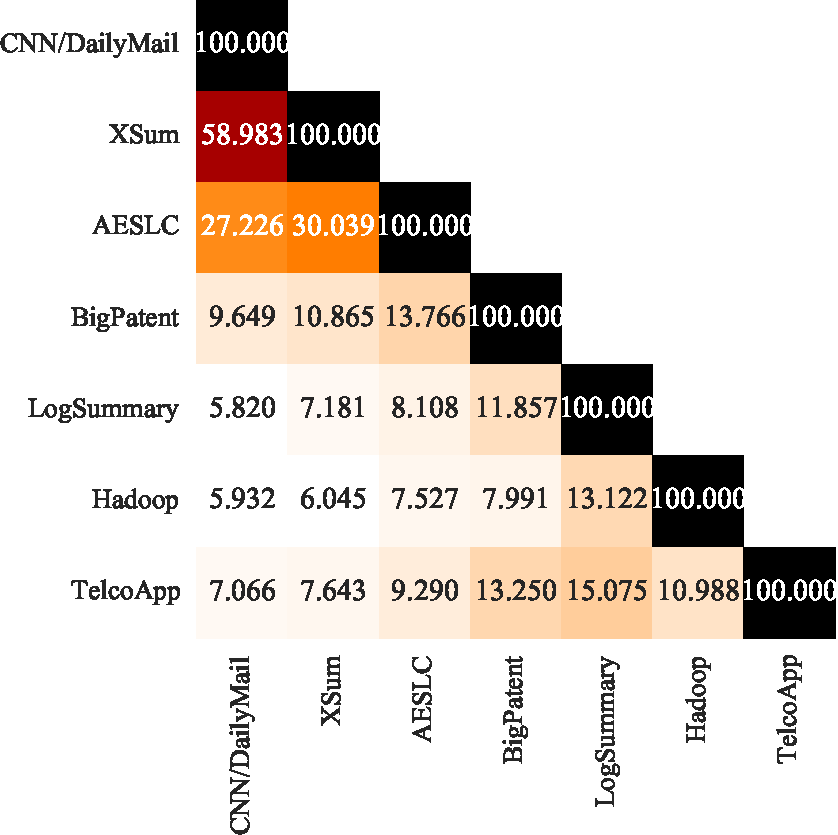
\includegraphics[width=.75\textwidth]{images/thesis/500_vocab_overlap_correlation}
\caption{Top 500 most frequent tokens (excluding stop words and infrequent tokens) shared among datasets from different domains.}
\label{fig:datasets_vocab_overlap}
\end{figure}

CNN/DailyMail and XSum share the highest amount of frequent tokens,
which is not unexpected as they are both datasets for news summarization.
AESLC shares a considerable amount of frequent tokens with those domains,
but otherwise the overlap between datasets is quite limited.

In general, the vocabulary of log datasets differs from that of other domains.
Log datasets show highest similarities between themselves,
but are quite diverse even among themselves.
A model performing well on one of these datasets might therefore not perform well on the other log datasets.
Interestingly, the vocabulary of BigPatent shows moderate similarity with \telco{} and \logsummary{},
which we find promising in respect to the transferability of log summarization.

\section{Investigating the Effects of Separators on Output Quality}\label{sec:preliminary_separators}

In \autoref{subsec:preprocessing} on \autopageref{subsubsec:model_input_challenges} we highlighted some challenges that come with
separating log messages from one another in the models' input;
Log messages often do not form complete sentences and thus punctuation cannot reliably be used for the purpose of separating messages.

Without such a separator it will be impossible for us to tell
where a model intends to end a log message and begin the next one,
as well as it being difficult for models to distinguish the semantic content of individual log messages.

In this section, we aim to find a sequence of tokens that can adequately serve as
separators for each model.

\subsection{Experimental setup}

Ideally, the separators we consider also have the function of separating text sequences
with different semantic content in the natural language corpora the models have been trained on.
We hypothesize that a model is more likely to understand that the additional tokens
are used to syntactically separate log messages which are text segments of different semantic contents.

We consider the following options:
\begin{description}
\item[\acs{bos}-/\acs{eos} tokens] These tokens are used to signify the beginning and end of the model's input.
      When fine-tuned for certain sentence-pair classification tasks \citeauthor*{bart} use their \ac{eos}-token as separator~\parencite[7874]{bart}.
      PEGASUS has a designated \ac{eos}-token only.

      This approach is equivalent to passing each log messages separately to a model's tokenizer and then manually concatenating the results.
\item[semicolons] Semicolons may be used in written text; usually they are used to separate two related but independent text segments.%
      \footnote{See \accessurl{https://www.grammarly.com/blog/semicolon/}{13.04.2022} for exemplified uses in the English language.}
      A semicolon used this way is typically separated by a space from the next word.
      BART's tokenizer makes the distinction between a semicolon with a subsequent space or without, while PEGASUS' does not.
\item[newlines] PEGASUS is able to encode newlines in its input,
      which separate paragraphs in the pre-training data.
      The special newline-token also has the benefit of not being contained in any log messages,
      as newlines typically separate different log-entries.
      Thus we can guarantee that newlines are only used to separate different log messages,
      while the model should still be familiar with the semantic meaning of a newline.
\end{description}
For better comparison we also include a space as a baseline to compare
model performances for when no special separator is employed.

We use \bart{-Large} and \pegasus{-Large} for this preliminary experiment,
which have not been fine-tuned to any specific task,
and train the models with the same setup as later in the \acs*{fsl} setting later described in \autoref{sec:evaluation_experiment_finetuned},
apart from the separator used to join log messages in the model inputs and reference summaries.
To be able to anticipate the effects of different separators on performance directly,
we decide to evaluate the models' text generation capabilities and against investigating perplexity.
Hence we perform a rough hyperparameter search to find \enquote{good-enough} parameters for the beam-search used to generate text.

\subsection{Results}

As the metric scores from this experiment are not meant to be comparable with the results from other experiments in this work,
but rather to evaluate different separators for each model individually,
we feel free to report the models' performance on a smaller, manually chosen validation set for each dataset.
(36, 25 and 11 examples for \logsummary{}, \hadoop{} and \telco{} respectively.)
Additionally we only report mean \(F_1\)-scores for \acs*{rouge}-1, \acs*{rouge}-2 and sentence-level \acs*{rouge}-L
since we are primarily focused on observing any relative improvements,
not conducting a comprehensive evaluation of the models.

We chose sentence-level \acs*{rouge}-L rather than summary-level,
as we are interested in the models ability to present the information in the same order as in the reference,
which would be ignored by summary-level \acs*{rouge}-L.

The results for BART are reported in \autoref{tab:separators_bart},
while the results for PEGASUS are shown in \autoref{tab:separators_pegasus}.
The best results are highlighted.

\begin{table}[htbp]
\centering
\footnotesize
\begin{tabular}{lccc}
                                 & \multicolumn{3}{c}{\scriptsize{}\acs*{rouge}-1 / \acs*{rouge}-2 / \acs*{rouge}-LSent}\\
                                 & \h{\logsummary{}}          & \h{\hadoop{}}              & \h{\telco{}}\\
\midrule
space (no syntactic separation)  & 71.6/63.2/68.2             & 35.5/31.6/34.1             & \h{43.8}/\h{37.1}/\h{38.7}\\
\acs{bos}-/\acs{eos}-token pair  & 55.9/45.0/53.3             & 33.7/28.0/31.0             & 35.1/27.5/27.6\\
% \acs{bos}-token                  & 51.2/33.3/50.2             & 42.0/34.8/39.5             & 38.4/31.0/33.8\\
semicolon with space             & 67.2/58.1/59.4             & 36.5/30.1/34.8             & 37.2/29.2/29.8\\
semicolon without space          & \h{72.4}/\h{65.7}/\h{70.4} & \h{47.6}/\h{40.2}/\h{45.2} & \h{43.8}/36.1/38.1\\
% double space                     & \h{77.5}/\h{68.4}/\h{71.6} & 37.5/31.1/35.2             & 30.7/23.5/26.5\\
\end{tabular}
\caption{Mean \acs*{rouge}-scores using \bart{-Large} with different separators across all validation sets.}
\label{tab:separators_bart}
\end{table}

\begin{table}[htbp]
\centering
\footnotesize
\begin{tabular}{lccc}
                                 & \multicolumn{3}{c}{\scriptsize{}\acs*{rouge}-1 / \acs*{rouge}-2 / \acs*{rouge}-LSent}\\
                                 & \h{\logsummary{}}          & \h{\hadoop{}}              & \h{\telco{}}\\
\midrule
space (no syntactic separation)  & 69.4/60.7/65.4             & 31.6/28.7/31.5             & 26.5/20.4/24.2\\
\acs{eos}-token                  & 51.8/42.3/51.8             & 21.9/18.9/21.8             & \phantom{0}7.6/\phantom{0}5.4/\phantom{0}7.1\\
semicolon                        & \h{77.0}/68.1/\h{72.7}     & \h{33.0}/\h{30.0}/\h{32.7} & 23.8/19.2/23.0\\
newline                          & 76.9/\h{68.8}/71.8         & 23.6/20.2/23.4             & \h{29.1}/\h{25.1}/\h{28.6}\\
\end{tabular}
\caption{Mean \acs*{rouge}-scores using \pegasus{-Large} with different separators across all validation sets.}
\label{tab:separators_pegasus}
\end{table}

We also report the ratio of log messages ending in a punctuation mark (one of \verb+.?!+) in \autoref{tab:sentence_endings},
and the ratio of log messages starting with a capital letter in \autoref{tab:capital_beginnings}.

\begin{table}[htbp]
\centering
\footnotesize
\begin{tabular}{ccc}
\h{\logsummary{}}                     & \h{\hadoop{}}                         & \h{\telco{}}\\
\midrule
\(\frac{311}{12020} \approx 2.587\%\) & \(\frac{233}{25931} \approx 0.899\%\) & \(\frac{592}{6079} \approx 9.738\%\)
\end{tabular}
\caption{Ratio of log messages ending in a punctuation mark across all datasets.}
\label{tab:sentence_endings}
\end{table}

\begin{table}[htbp]
\centering
\footnotesize
\begin{tabular}{ccc}
\h{\logsummary{}}                       & \h{\hadoop{}}                            & \h{\telco{}}\\
\midrule
\(\frac{5479}{12020} \approx 45.582\%\) & \(\frac{23550}{25931} \approx 90.818\%\) & \(\frac{1970}{6079} \approx 32.407\%\)
\end{tabular}
\caption{Ratio of log messages starting with a capitalized token across all datasets.}
\label{tab:capital_beginnings}
\end{table}

\subsection{Discussion}

Generally, \acs{bos}-/\acs{eos}-tokens perform poorly as separators,
in all cases performing worse than providing no syntactical separation of log messages.
The poor performance can at least in part be explained by the fact
that \acs{eos}-tokens signify to the beam-search that a beam is finished.
When manually inspecting the generated summaries, we notice they are particularly short,
leading to low recall, resulting in a low overall score.

In most cases, providing some form of separators significantly improved performance compared to using no explicit syntactical separation,
confirming our assumption that it is important for models to be able to differentiate between different log messages.
In settings where spaces performed comparatively well,
we suspect that models may be able to use existing patterns concerning punctuation or capitalization to distinct between log messages.

\paragraph{PEGASUS}

We observe that \pegasus{-Large} clearly benefits from the use of explicitly inserted separators on every dataset.
This can be seen well on the \logsummary{}-dataset,
where either option resulted in a minimum of a \(9.79\%\) increase in model performance after training (among all observed metrics)
compared to separating subsequent log messages by a space.

Interestingly, not providing additional syntactical separation by using spaces as separators
performs well with \hadoop{}.
We believe this can in part be explained by the consistent use of capitalization in this dataset,
as signified by the high rate of capital letters at the beginning of log messages.
Our hypothesis is that \pegasus{-Large} picked up on this pattern and it is sufficient for it to identify semantically different text segments.

On the other hand, the low amount of punctuation at the end of log messages seen in \hadoop{}
may be the reason why using a punctuation-symbol such as semicolons performs better than using newlines in this specific case,
whereas introducing extra punctuation performs worse in cases where punctuation is already present,
such as \telco{}.

\paragraph{BART}

With \bart{-Large}, the benefits of introducing explicit separators seem less pronounced
considering that spaces almost as well as the best choice for \logsummary{} and the best for \telco{}.

However, we do also see a minimum of \(27.22\%\) performance increase for all considered metrics on the \hadoop{}-dataset
when using semicolons without additional spaces compared to using spaces for separation.\\
This shows to us that \bart{-Large} also benefits from being able to differentiate between independent log messages,
at least in cases where there is a lack of punctuation at the end of messages.

Oddly enough, inserting a semicolon followed by a space between each log message,
as one would do to separate independent text segments in a sentence, performs poorly.
We are unsure why the model prefers semicolons without subsequent spaces,
although we will highlight that the semicolon is represented by different tokens with different embeddings
depending on whether a space is inserted or not.
This means that the model did not necessarily learn that these two tokens have the same meaning for humans,
instead there may be some biases present in the pre-training data that make the semicolon without a space
a better syntactic separator of semantically independent text segments.

\paragraph{Conclusion}

It is impracticable to evaluate all possible tokens as separators.
Hence, there may be some other sensible choices
we did not consider that are better suited for use as separators.
Furthermore, models previously fine-tuned may prefer different separators depending on the patterns seen in their domain and dataset.
Nevertheless, performing such a preliminary study for each fine-tuned summarization model from \autoref{tab:finetuned_models_overview}
individually would be an impractical effort;
instead we rely on the assumption that previously fine-tuned models inherit some knowledge on separators from their pre-trained bases.

Our goal was not to find optimal separators for our models,
but to find ones that produce adequate results.
Ideally, we would like to choose a single option per model going forward and use it consistently across all datasets.
It would allow for models to be used in more universal settings.

We make an exception for this rule with PEGASUS-models:
We choose newlines as separators for \logsummary{} and \telco{}-datasets,
but use semicolons on the \hadoop{}-dataset
because we see a significant \(39.74\%\) increase among all observed metrics compared to newlines.

For BART-models we decide on semicolons as separators (without inserting a space after each semicolon)
for all datasets, even if slightly outperformed by using regular spaces on \telco{}.

As not introducing additional syntactic separation makes it harder to tell apart independent text segments in the summary
and therefore decreases readability,
we believe using spaces as separators is less helpful for any human operators using the model as it,
even if the performance is comparatively good when considering \acs*{rouge} metrics.

\section{Evaluation of Summarization Models from other Domains}\label{sec:evaluation_experiment_finetuned}

As motivated in \autoref{subsubsec:approch_experiment_1},
we aim to determine if models fine-tuned for summarization on other previously researched domains
are able to transfer their knowledge on summarization to log-data.

For this, we evaluate all models laid out in \autoref{tab:finetuned_models_overview}
on \autopageref{tab:finetuned_models_overview}
in a \ac{zsl} and a \ac{fsl} setting.
Additionally, we include the baseline models \bart{-Large} and \pegasus{-Large}
which have not been fine-tuned on summarization before.
This way, we can see if previous fine-tuning for summarization makes a noticeable difference in performance,
or if it suffices to fine-tune on the limited data available.

Under ideal circumstances we could simply let each of the models generate summaries on all our datasets.
Using the \acs*{rouge}-metrics we could then quantify the performance of the models
and conclude if any singular model outperforms the others.

During preliminary experiments, however, we find that the length of generated text heavily
depends on the parameter chosen for the beam-search,
such as constraints on the minimum and maximum amount of tokens generated
and the \emph{length penalty} in particular.
The length of the summary directly influences its quality according to the \acs*{rouge}-metrics;
As such we would need to find optimal values for such parameters influencing the generation of text
in order to keep a fair comparison between models.
Unfortunately, each model variant appears to have their own optima for such generation-parameters on every dataset.

Because finding optimal values for these parameters for each model is error-prone and cumbersome,
we instead choose to initially focus on the perplexity for comparing different models,
then compare generated summaries for selected models only.

Sometimes we employ boxplots to visualize our results;
these are the classic \enquote{Tukey} boxplots~\parencite{boxplots},
with a red line indicating the median of the distribution.
Similarly, we use violin plots that visualize the data's distribution density,
using the same indication of the median.
Both types of plots and their origins are explained in \parencite{boxplots}.

We include intermediate results and frequently draw similar conclusions from different perspectives.
We believe this to be necessary to justify the decisions we take in presenting the final results,
but as a consequence, this section may be a bit long-winded.\\
As such we summarize any important intermediate conclusions during the final discussion of this experiment in
\autoref{subsec:evaluation_experiment_finetuned_discussion}.

\subsection{Experimental Setup}

During the experiments in the next segments,
we regularly evaluate models in two different settings with differing levels of supervision;
With further fine-tuning on the training dataset or without:

\paragraph{\acf*{zsl} setting}

As described in \autoref{subsec:training_test_split}
we defined a set of training examples for each dataset and use the rest for evaluation.

A \acl{zsl} setting means that the models have previously seen zero training examples on the concrete task/dataset used;
as such we simply run the models on the test datasets and evaluate their outputs,
either through perplexity or through examining their summaries generated via beam-search.

Following \citeauthor*{bart} and \citeauthor*{pegasus} we apply a label smoothing factor of \(0.1\)
for computing the cross-entropy loss~\parencites[7876]{bart}[appendix]{pegasus},
which impacts the perplexity scores.

\paragraph{\acf*{fsl} setting}

In the \ac{fsl} setting we first train the models on a small training set,
minimizing the cross-entropy between model predictions and reference summaries,
and then evaluate it on the same test set as described above.

We use an effective batch-size of 8 and using a constant learning rate of \(5 \cdot 10^{-5}\) we train for different amount of steps on each dataset:
\begin{description}[nosep, itemsep=1ex, labelwidth=\widthof{\logsummary}, leftmargin=\labelwidth+\labelsep, align=parright]
\item[\logsummary] \(20 \cdot \left\lceil\frac{30}{8}\right\rceil = 80\)
\item[\hadoop]     \(15 \cdot \left\lceil\frac{50}{8}\right\rceil = 105\)
\item[\telco]      \(25 \cdot \left\lceil\frac{16}{8}\right\rceil = 50\)
\end{description}
where the number of steps is determined as
\begin{equation}
\text{\#steps} = \text{\#epochs} \cdot \left\lceil\frac{\text{\#training-examples}}{\text{batch-size}}\right\rceil
\end{equation}
An epoch is understood as an iteration over the entire training dataset.
We chose an adequate number of epochs using our experiences from preliminary trials,
where we observed roughly at which point the generation
performance starts to stagnate or even deteriorate on a validation set
and chose an amount of epochs that works for \emph{both} model architectures.

\subsection{Analysis of Model Perplexities}

We first evaluate the perplexity of the models only.
Again, perplexities are not comparable between models with different vocabularies
for the reasons laid out in \autoref{sec:perplexity}.
However, we can compare models of the same architecture,
e.g. \bart{-Large} with \bart{-CNN} as they use the same vocabulary and tokenizer.

The results for BART are shown in \autoref{tab:bart_zsl_perplexities} for the \acl{zsl} setting
and in \autoref{tab:bart_fsl_perplexities} for the \acl{fsl} setting.

\begin{table}[htbp]
\centering
\footnotesize
\begin{tabular}{lrrr}
              & \h{\logsummary{}} & \h{\hadoop{}} & \h{\telco{}}\\
\midrule
\bart{-Large} & 869.696           & 19.356        & 31.837\\
\bart{-CNN}   & \h{89.208}        & \h{5.447}     & \h{7.373}\\
\bart{-XSum}  & 412.338           & 10.316        & 11.844\\
\end{tabular}
\caption{Perplexities of BART variants in a  \acl*{zsl} setting.}
\label{tab:bart_zsl_perplexities}
\end{table}

\begin{table}[htbp]
\centering
\footnotesize
\begin{tabular}{lrrr}
              & \h{\logsummary{}} & \h{\hadoop{}} & \h{\telco{}}\\
\midrule
\bart{-Large} & \h{15.547}    & 4.581         & 7.151\\
\bart{-CNN}   & 17.236        & \h{4.369}     & \h{6.009}\\
\bart{-XSum}  & 15.820        & 4.518         & 7.032\\
\end{tabular}
\caption{Perplexities of BART variants in a  \acl*{fsl} setting.}
\label{tab:bart_fsl_perplexities}
\end{table}

For PEGASUS we report the \acl{zsl} results in \autoref{tab:pegasus_zsl_perplexities}
and in \autoref{tab:pegasus_fsl_perplexities} for the \acl{fsl} setting.

\begin{table}[htbp]
\centering
\footnotesize
\begin{tabular}{lrrr}
                     & \h{\logsummary{}} & \h{\hadoop{}} & \h{\telco{}}\\
\midrule
\pegasus{-Large}     & 1684.929      & \h{100.972}   & \h{168.063}\\
\pegasus{-CNN}       & 563.526       & 136.606       & 173.432\\
\pegasus{-XSum}      & \h{495.076}   & 525.619       & 459.367\\
\pegasus{-AESLC}     & 747.233       & 703.096       & 744.069\\
\pegasus{-BigPatent} & 1399.012      & 705.201       & 330.518\\
\end{tabular}
\caption{Perplexities of PEGASUS variants in a  \acl*{zsl} setting.}
\label{tab:pegasus_zsl_perplexities}
\end{table}

\begin{table}[htbp]
\centering
\footnotesize
\begin{tabular}{lrrr}
                     & \h{\logsummary{}} & \h{\hadoop{}} & \h{\telco{}}\\
\midrule
\pegasus{-Large}     & 12.957        & 6.115         & 32.345\\
\pegasus{-CNN}       & \h{12.244}    & \h{5.559}     & \h{27.920}\\
\pegasus{-XSum}      & 13.144        & 9.560         & 78.193\\
\pegasus{-AESLC}     & 19.775        & 8.943         & 68.682\\
\pegasus{-BigPatent} & 60.724        & 29.735        & 108.614\\
\end{tabular}
\caption{Perplexities of PEGASUS variants in a  \acl*{fsl} setting.}
\label{tab:pegasus_fsl_perplexities}
\end{table}

Generally, we notice that previous fine-tuning on summarization data does help when in a \ac{zsl} setting,
but the differences between models shrink significantly after training on the few examples provided.

This is especially true for BART models,
for which the largest relative deviation between the best and lowest scoring models after fine-tuning is
approximately \(11\%\) on the \logsummary{}, \(5\%\) on the \hadoop{} and \(19\%\) on the \telco{}-dataset.
(Which is low compared to for example \(\approx 255\%\) on the \hadoop{} dataset for \ac{zsl}.)
While judging the perplexity alone is not enough to infer a models performance to generate good summaries,
this is a strong indicator that previous training for summarization
does not contribute considerably to a models ability to predict summaries on our specific log-data.

This also holds for PEGASUS, where \pegasus{-Large} always shows the second-best performance,
with an approximate relative derivation of \(6\%\), \(10\%\) and \(16\%\)
from \pegasus{-CNN} on \logsummary{}, \hadoop{} and \telco{} respectively.

However, we can see that using previously fine-tuned models
can actually perform substantially worse than the baseline \pegasus{-Large}.
Especially the variant fine-tuned for summarization on BigPatent failed to achieve similar perplexities as the other variants,
despite the higher overlap of vocabulary we found in \autoref{subsec:other_domains_vs_log_datasets}.
As summaries in BigPatent tend to be abstractive~\parencite[2204-2205]{bigpatent},
we suspect that the model is unable to quickly adapt to a more extractive task such as the ones presented by us.
\pegasus{-BigPatent} may improve further with more fine-tuning steps,
but even so, \pegasus{-Large} managed to adapt much quicker:
Initially staring with a higher perplexity in the \ac{zsl} setting,
but achieving a significantly better \ac{fsl} result after the same amount of training-steps on \logsummary{}.
This reinforces our assessment that further fine-tuning models previously trained on summarization tasks
is not worth it for dissimilar domains such as log-data
and that fine-tuning pre-trained models even with only a few examples is sufficient.

Still, for both models the best performing \ac{fsl} model
is most often the variant trained on the CNN/DailyMail dataset,
albeit closely followed by the baselines \bart{-Large} and \pegasus{-Large}.

Extractive models tend to perform better on the CNN/DailyMail news-dataset than abstractive ones~\parencite[547]{summarization_critical_evaluation},
which may explain why models fine-tuned on this dataset outperform those trained on other domains.
After all, the summaries in all our log summarization datasets are purely extractive,
hence do not include any novel words not seen in the input data or any paraphrasation of content.
The slight difference in performance compared to the baselines not tuned for summarization
might indicate that there is still some insight to gain concerning which text segments are relevant.
We believe this is why we are seeing that \bart{-CNN} performs comparatively well in a \ac{zsl} setting.

As noted before, lower perplexity usually correlates with better performance in applications,
but if the model simply gets more confident in more obvious cases, this is not always the case.
Hence we cannot be sure that the models showing the best perplexities
are also the ones performing the best for summarization of our log-data.
To select the best models, we conduct a few further trials before decide on the final models to evaluate.

\subsection{Further Trials to determine the best Models}

\paragraph{PEGASUS}
Due to the summary length heavily impacting the recall of the \acs*{rouge} metric,
and the complications arising from optimizing the summary length using the parameters of the beam-search,
we instead decide to compare only the \acs*{rouge} precision
while setting the length of generated summaries to a small, fixed amount.
For the PEGASUS models we decide on the following lengths:
\begin{itemize}
\item We let the models generate exactly 20 tokens on the \telco{} and \hadoop{} datasets.
\item On the \logsummary{} dataset, we instruct the model to generate only 8 tokens,
      as summaries are much shorter in this dataset.
      8 tokens corresponds to the median length of summaries using PEGASUS' tokenizer.
\end{itemize}

By comparing the precision only, we can judge what percentage of the few written tokens are actually relevant.
Thus we hope to anticipate the performance of the models when scaled up to the full summarization task
and select a well-performing model.

The mean \(F_1\)-scores for \acs*{rouge}-1, \acs*{rouge}-2 and sentence-level \acs*{rouge}-L
are reported in \autoref{tab:pegasus_trial_zsl} for the \ac{zsl} setting
and in \autoref{tab:pegasus_trial_fsl} for the \ac{fsl} one.

\begin{table}[htbp]
\centering
\footnotesize
\begin{tabular}{lccc}
                     & \multicolumn{3}{c}{\scriptsize{}\acs*{rouge}-1 / \acs*{rouge}-2 / \acs*{rouge}-LSent}\\
                     & \h{\logsummary{}}          & \h{\hadoop{}}              & \h{\telco{}}\\
\midrule
\pegasus{-Large}     & 50.9/27.2/48.2             & 75.3/\h{72.6}/75.1         & \h{43.3}/\h{34.2}/\h{42.9}\\
\pegasus{-CNN}       & \h{58.9}/\h{32.9}/\h{55.1} & \h{77.8}/70.8/\h{77.7}     & 39.5/27.2/37.9\\
\pegasus{-XSum}      & 41.0/25.5/39.3             & 66.0/60.9/65.6             & 26.9/12.0/24.9\\
\pegasus{-AESLC}     & 41.8/23.7/39.5             & 46.1/33.4/45.9             & 31.0/15.4/29.3\\
\pegasus{-BigPatent} & 15.7/\phantom{0}8.5/14.9   & 25.3/\phantom{0}5.0/25.1   & 14.3/\phantom{0}2.0/11.7\\
\end{tabular}
\caption{Mean \acs*{rouge} precisions of \ac*{zsl} PEGASUS models in a constrained summarization task.}
\label{tab:pegasus_trial_zsl}
\end{table}

\begin{table}[htbp]
\centering
\footnotesize
\begin{tabular}{lccc}
                     & \multicolumn{3}{c}{\scriptsize{}\acs*{rouge}-1 / \acs*{rouge}-2 / \acs*{rouge}-LSent}\\
                     & \h{\logsummary{}}          & \h{\hadoop{}}              & \h{\telco{}}\\
\midrule
\pegasus{-Large}     & \h{82.5}/\h{70.7}/\h{78.3} & \h{94.2}/\h{93.4}/\h{94.1} & \h{49.4}/\h{38.6}/\h{48.5}\\
\pegasus{-CNN}       & 81.0/69.6/77.9             & 93.5/82.7/89.6             & 44.3/32.3/43.1\\
\pegasus{-XSum}      & 81.7/69.4/77.6             & 92.9/89.7/92.7             & 45.4/30.0/43.2\\
\pegasus{-AESLC}     & 79.0/64.6/75.3             & 92.5/91.1/92.4             & 47.7/31.1/45.9\\
\pegasus{-BigPatent} & 49.8/34.1/48.5             & 46.4/29.7/44.7             & 32.9/19.5/29.9\\
\end{tabular}
\caption{Mean \acs*{rouge} precisions of \ac*{fsl} PEGASUS models in a constrained summarization task.}
\label{tab:pegasus_trial_fsl}
\end{table}

We observe that the perplexity of a model does not perfectly match its performance in this constrained summarization setting:
In the \ac{zsl} setting, \pegasus{-Large} performs second-best on \telco{} despite previously showing the highest perplexity.
On the other side of the spectrum, \pegasus{-BigPatent} performs worse than its perplexity would indicate;
for example in the \telco{}-dataset where the \ac{fsl} BigPatent model performs about as good
as the AESLC model in the \ac{zsl} setting,
despite \pegasus{-BigPatent} now exhibiting a perplexity that is about 7 times lower than \ac{zsl} \pegasus{-AESLC}.

Unsurprisingly, the models perform much better in a \ac{fsl} setting after being fine-tuned on a few examples.
We explore the quality of these generated texts in an example from the \logsummary{}-dataset in \autoref{tab:logsummary_pegasus_example_1}.

\begin{table}[htbp]
\centering
\footnotesize
\setlength{\tabcolsep}{.5ex}
\begin{tabularx}{\textwidth}{XXXXX}
\toprule
\multicolumn{4}{c}{\textbf{input}}
&\textbf{reference summary}\\
\midrule
\multicolumn{4}{p{.75\textwidth}}{
\tiny
\ttfamily\hbadness=10000
Accepted socket connection from remote host \#83617

Connection request from old client remote host \#83617 ; will be dropped if server is in r-o mode

Client attempting to establish new session at remote host \#83617

Established session 238367163526545476 with negotiated timeout 10000 for client remote host \#83617

\textelp{} \textit{(messages repeat with 4 different clients)}}
&
\tiny
\ttfamily\hbadness=10000
Accepted socket connection

Connection request

Established session timeout
\\
\midrule
\h{\pegasus{-Large}}
&\h{\pegasus{-CNN}}
&\h{\pegasus{-XSum}}
&\h{\pegasus{-AESLC}}
&\h{\pegasus{-BigPat.}}\\
\tiny\acs*{rouge}-LSent precision: \(100\)
&\tiny\acs*{rouge}-LSent precision: \(60\)
&\tiny\acs*{rouge}-LSent precision: \(16.7\)
&\tiny\acs*{rouge}-LSent precision: \(40\)
&\tiny\acs*{rouge}-LSent precision: \(33.3\)\\
\midrule
\tiny
\ttfamily\hbadness=10000
Accepted socket connection

Established session
&
\tiny
\ttfamily\hbadness=10000
Accepted socket connection

Client attempting
&
\tiny
\ttfamily\hbadness=10000
Client attempting to establish new session
&
\tiny
\ttfamily\hbadness=10000
Connection request from old client
&
\tiny
\ttfamily\hbadness=10000
A socket request from old client\\
\bottomrule
\end{tabularx}
\caption{\ac*{fsl} predictions on an example from the \emph{ZooKeeper}-subdataset of \logsummary{}.}
\label{tab:logsummary_pegasus_example_1}
\end{table}

We find that, at least with this example,
models originating from a more abstractive summarization background prefer to include grammatically sound segments in their summary,
as can be seen for \pegasus{-XSum} and \pegasus{-BigPatent}.

\pegasus{-BigPatent}'s summary is the most abstractive one, combining two different log messages into a single statement.
This hurts its score on the \acs{rouge} metric, even if the summary is analogous to the one from \pegasus{-AESLC},
and explains why this model performs poorly regarding this metric.

However, this more abstractive approach is also more error-prone.
In another example, \autoref{tab:logsummary_pegasus_example_2}, \pegasus{-BigPatent} includes additional descriptive text,
which does not fit the context of the log:
\verb+binding to port+ is an action taken by the software producing the log,
but similar to the summaries of patents in the BigPatent dataset,
the model seems to interpret the log as a procedure that needs to be described.

Therefore we do not believe that abstractive models perform worse solely because the \acs*{rouge} metric prefers extractive summaries,
but because they do not fully understand the log-data presented to them and fail to interpret it in a meaningful way;
even more so as they have not been provided with abstractive summaries during fine-tuning.
Ultimately we think a purely extractive summary in the style of the human-written summaries of this dataset will be more helpful to any human operator
than a factually inconsistent abstractive description of what happened.

Hence why we decide to select the \pegasus{-Large} model for further evaluation:
Comparing \autoref{tab:pegasus_trial_fsl} and \autoref{tab:pegasus_trial_zsl}, it outperforms every other variant in the \ac{fsl} setting and is competitive in the \ac{zsl} setting.
As can be seen from the examples, its summaries follow the extractive style of the human-written summaries.

\pegasus{-CNN} would be another viable alternative, as it shows even better perplexity,
but evidently it performs slightly worse in this constrained generation setting.
We speculate this is the case because \pegasus{-Large} can more quickly adapt to the summarization task,
as it does not have any prior biases towards which parts of the input document need to be included in the summary.
Previous research has shown that summarization of news articles is prone to substantial layout biases~\parencite[544]{summarization_critical_evaluation},
speaking against the use of previously fine-tuned models such as \pegasus{-CNN},
which is accustomed to summarizing news articles.

\begin{table}[htbp]
\centering
\footnotesize
\setlength{\tabcolsep}{.5ex}
\begin{tabularx}{\textwidth}{XXXXX}
\toprule
\multicolumn{4}{c}{\textbf{input}}
&\textbf{reference summary}\\
\midrule
\multicolumn{4}{p{.75\textwidth}}{
\tiny
\ttfamily\hbadness=10000
binding to port remote host \#44607remote host \#5137

tickTime set to 2000

minSessionTimeout set to -1

maxSessionTimeout set to -1

initLimit set to 10

Reading snapshot zookeeper

My election bind port : remote host \#44607remote host \#47103

LOOKING

New election. My id = 1 , proposed zxid = 30064771479

Notification : 1 ( n.leader ) , 30064771479 ( n.zxid ) , 1 ( n.round ) , LOOKING ( n.state ) , 1 ( n.sid ) , 7 ( n.peerEPoch ) , LOOKING ( my state )

Have smaller server identifier , so dropping the connection : ( 2 , 1 )

Received connection request remote host \#46154

Have smaller server identifier , so dropping the connection : ( 3 , 1 )

Received connection request remote host \#7574

Notification : 3 ( n.leader ) , 30064771479 ( n.zxid ) , 1 ( n.round ) , LOOKING ( n.state ) , 2 ( n.sid ) , 7 ( n.peerEPoch ) , LOOKING ( my state )

\textelp{} \textit{(4 similar messages discarded in this example for brevity)}

Notification : 3 ( n.leader ) , 30064771479 ( n.zxid ) , 1 ( n.round ) , FOLLOWING ( n.state ) , 2 ( n.sid ) , 7 ( n.peerEPoch ) , LOOKING ( my state )
}
&
\tiny
\ttfamily\hbadness=10000
binding to port

Reading snapshot

Have smaller server identifier

dropping the connection

Received connection request
\\
\midrule
\h{\pegasus{-Large}}
&\h{\pegasus{-CNN}}
&\h{\pegasus{-XSum}}
&\h{\pegasus{-AESLC}}
&\h{\pegasus{-BigPat.}}\\
\tiny\acs*{rouge}-LSent precision: \(100\)
&\tiny\acs*{rouge}-LSent precision: \(40\)
&\tiny\acs*{rouge}-LSent precision: \(60\)
&\tiny\acs*{rouge}-LSent precision: \(100\)
&\tiny\acs*{rouge}-LSent precision: \(50\)\\
\midrule
\tiny
\ttfamily\hbadness=10000
Have smaller server identifier

Received
&
\tiny
\ttfamily\hbadness=10000
bind to port remote host
&
\tiny
\ttfamily\hbadness=10000
My state

Received connection request
&
\tiny
\ttfamily\hbadness=10000
binding to port

Received connection
&
\tiny
\ttfamily\hbadness=10000
A method for binding to port\\
\bottomrule
\end{tabularx}
\caption{\ac*{fsl} predictions on a more diverse example from the \emph{ZooKeeper}-subdataset of \logsummary{}.}
\label{tab:logsummary_pegasus_example_2}
\end{table}

\paragraph{BART}
For the BART variants, the performances on this constrained generation task do not differ significantly between models,
so we chose to omit the results here.
Instead, we did perform a hyperparameter search for all variants on the \logsummary{} task,
where the generated summaries are the shortest,
and thus the search can evaluate different parameters in a relatively timely manner.
To further speed up the search,
it is performed on a manually selected validation set and not the whole dataset,
resulting in 20 trials to determine an optimal length penalty.
The resulting \acs*{rouge}-2 and summary-level \acs*{rouge}-L metrics on the evaluation dataset are visualized
in \autoref{fig:bart_trial_zsl_logsummary} (\acs{zsl}) and \autoref{fig:bart_trial_fsl_logsummary} (\acs{fsl}).

\begin{figure}[htbp]
\centering
\subfloat[\bart{-Large}]{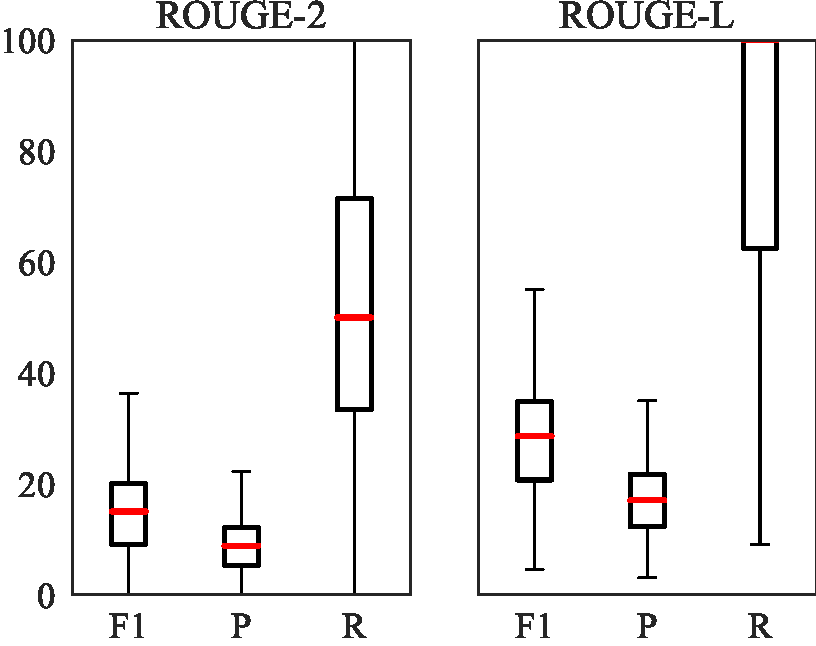
\includegraphics[width=.32\textwidth]{images/thesis/result_boxplots/logsummary_bart-large-zsl}}%
\hfill{}%
\subfloat[\bart{-CNN}]{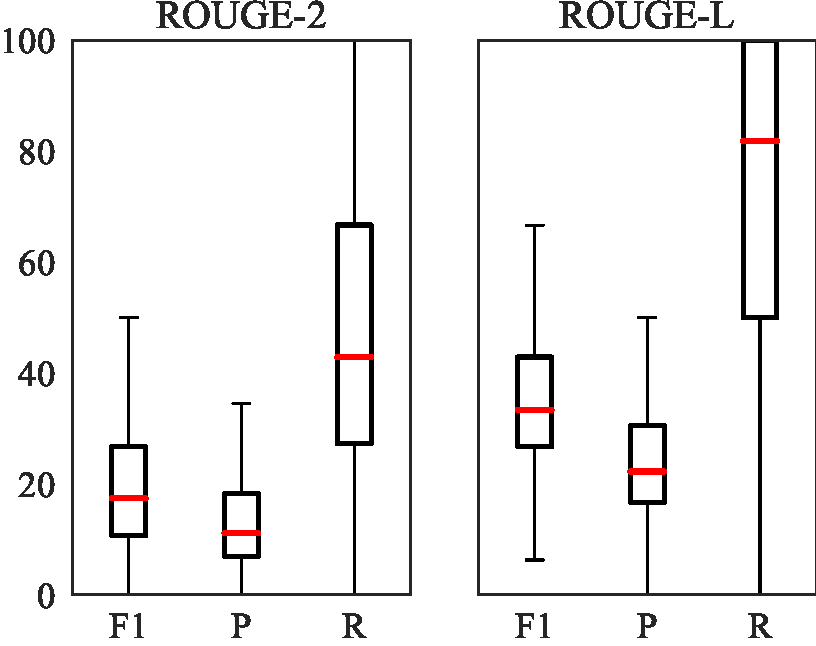
\includegraphics[width=.32\textwidth]{images/thesis/result_boxplots/logsummary_bart-large-cnn-zsl}}%
\hfill{}%
\subfloat[\bart{-XSum}]{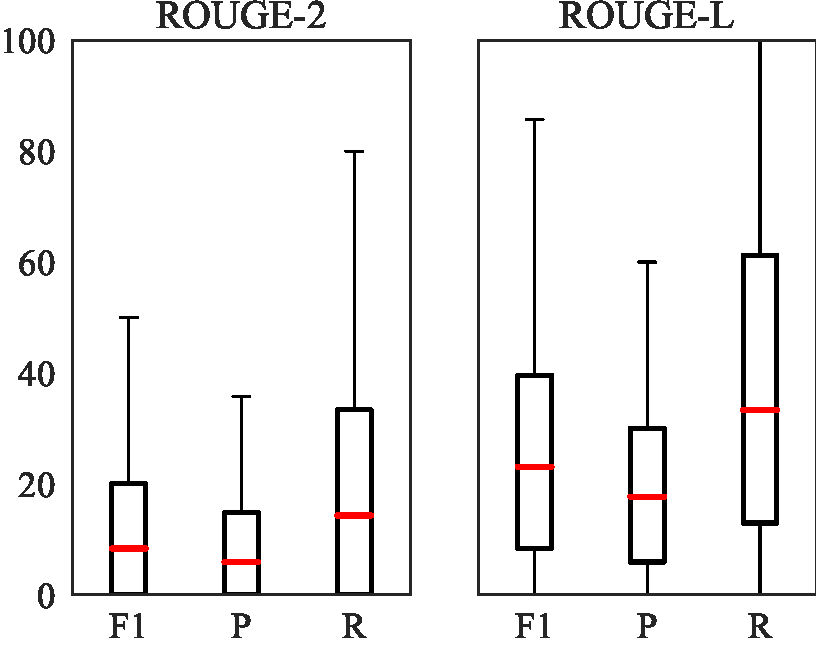
\includegraphics[width=.32\textwidth]{images/thesis/result_boxplots/logsummary_bart-large-xsum-zsl}}
\caption{Boxplots showing \acs*{rouge} recall, precision and \(F_1\)-scores
for different BART variants without further fine-tuning (\acs*{zsl}) on the \logsummary{} dataset.}
\label{fig:bart_trial_zsl_logsummary}
\end{figure}

\begin{figure}[htbp]
\centering
\subfloat[\bart{-Large}]{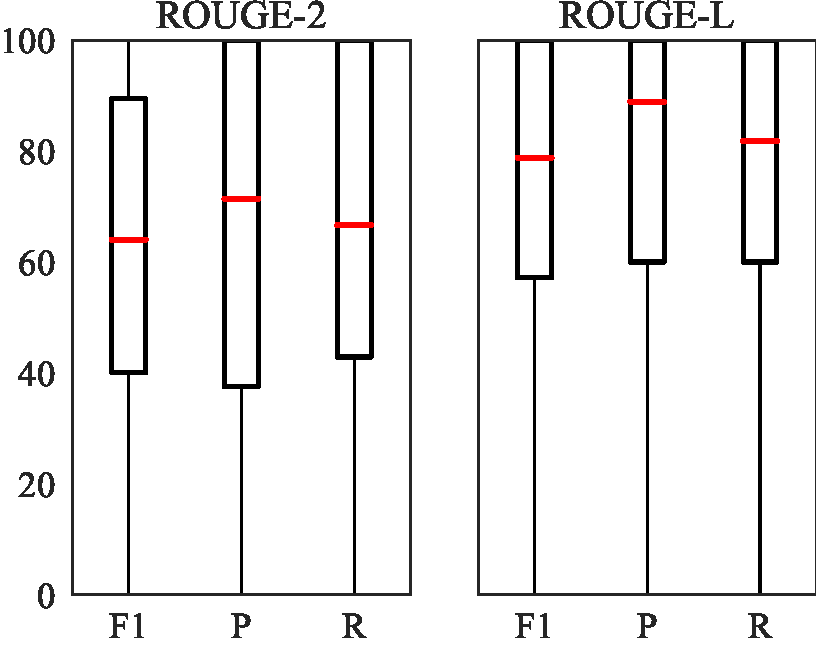
\includegraphics[width=.32\textwidth]{images/thesis/result_boxplots/logsummary_bart-large}}%
\hfill{}%
\subfloat[\bart{-CNN}]{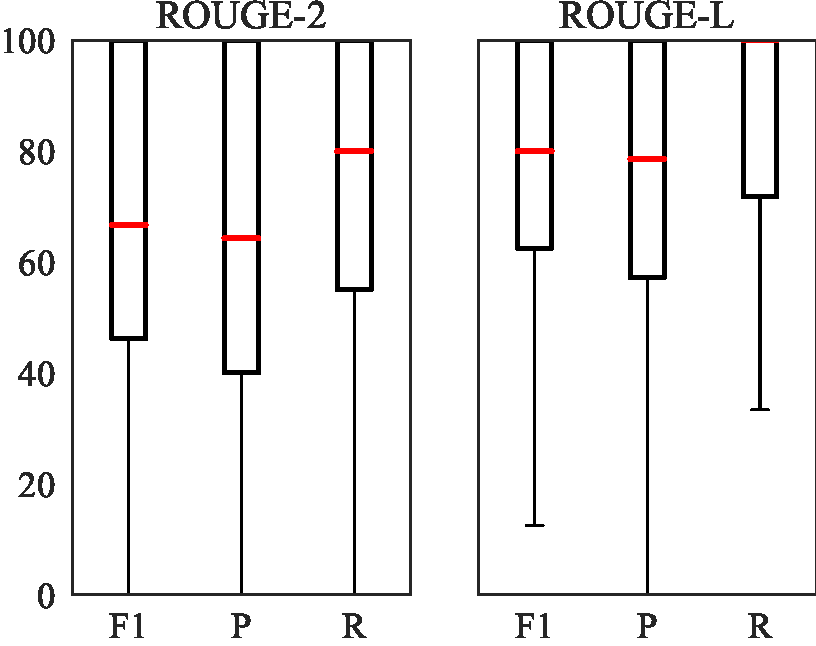
\includegraphics[width=.32\textwidth]{images/thesis/result_boxplots/logsummary_bart-large-cnn}}%
\hfill{}%
\subfloat[\bart{-XSum}]{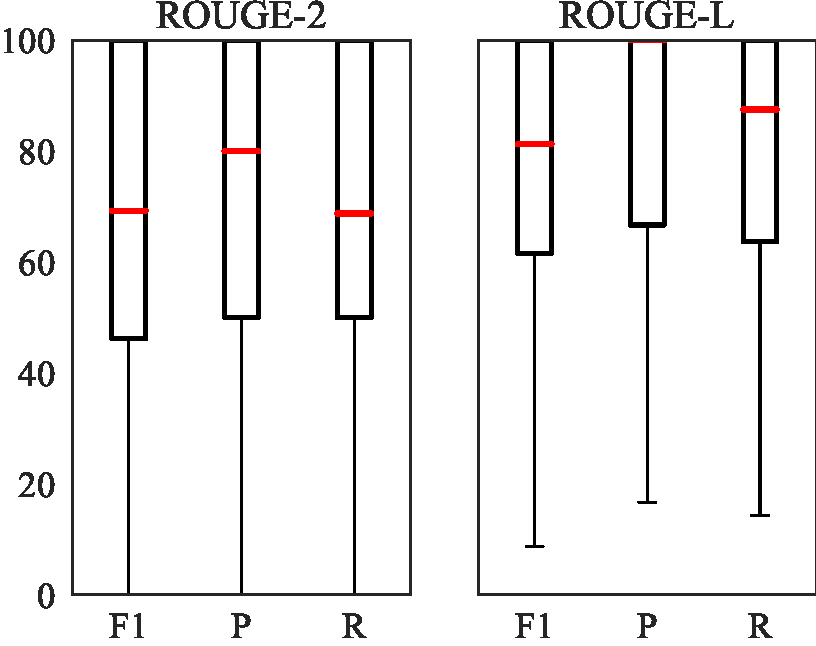
\includegraphics[width=.32\textwidth]{images/thesis/result_boxplots/logsummary_bart-large-xsum}}
\caption{Boxplots showing \acs*{rouge} recall, precision and \(F_1\)-scores
for different BART variants that have been further fine-tuned (\acs*{fsl}) on the \logsummary{} dataset.}
\label{fig:bart_trial_fsl_logsummary}
\end{figure}

In addition, we decide to qualitatively evaluate a summary generated in a \ac{zsl} setting,
and compare it to a summary written after fine-tuning.
To determine the models ability to select the log messages deemed relevant by the human-written reference,
we choose an example whose \ac{zsl}-prediction scores nearest to the median of
summary-level \acs*{rouge}-L recall on the \emph{Spark}-subdataset of \logsummary{}.
The precision would also measure the summary's conciseness, hence why we decide against using the \(F_1\)-score in this case.
We show the input, human-written summary
and \bart{-CNN}'s predictions in \autoref{tab:logsummary_bart_cnn_example}.
\bart{-CNN} is the BART-model that performed best in a \ac{zsl} setting according to perplexity.
For the \ac{zsl}-prediction we highlight the portions of the generated summary that correspond to the reference.

\begin{table}[htbp]
\centering
\footnotesize
%\setlength{\parskip}{0pt}\setlength{\parindent}{-1em}\setlength{\leftskip}{1em}
\begin{tabularx}{\textwidth}{>{\ttfamily\hbadness=10000}X>{\ttfamily\hbadness=10000}p{.2\textwidth}}
\toprule
\normalfont\textbf{input}
&\normalfont\textbf{reference summary}\\
\midrule
\tiny
Block rdd stored as bytes in memory ( estimated size 16.0 B , free 6.2 MB )

Block rdd stored as bytes in memory ( estimated size 16.0 B , free 6.2 MB )

Times : total = 38 , boot = 16 , init = 22 , finish = 0

Times : total = 37 , boot = 20 , init = 17 , finish = 0

Times : total = 38 , boot = 16 , init = 22 , finish = 0

Times : total = 38 , boot = 16 , init = 22 , finish = 0

Times : total = 38 , boot = 21 , init = 17 , finish = 0

Finished task 14.0 in stage 1359.0 ( TID 54654 ) . 2667 bytes result sent to driver

\textelp{} \textit{(4 similar messages discarded in this example for brevity)}

Got assigned task 54656

Running task 15.0 in stage 1359.0 ( TID 54656 )

\textelp{} \textit{(3 similar messages discarded in this example for brevity)}
&
\tiny
Running task

Finished task

Got assigned task

Block stored in memory
\\
\midrule
\normalfont\textbf{\bart{-CNN} \acs{zsl}}
&\normalfont\textbf{\bart{-CNN} \acs{fsl}}\\
\normalfont\tiny\acs*{rouge}-L recall: \(54.54\)
&\normalfont\tiny\acs*{rouge}-L recall: \(100\)\\
\midrule
\tiny
\h{\emph{Block}} rdd \h{\emph{stored}} as bytes \h{\emph{in memory}} ( estimated size 16.0 B, free 6.2 MB )

Times : total = 38, boot = 16, init = 22, finish = 0

\h{\emph{Finished task}} 14.0 in stage 1359.0 ( TID 54654 ). 2667 bytes result sent to driver
&
\tiny
Block stored in memory

Finished task

Running task

Got assigned task
\\
\bottomrule
\end{tabularx}
\caption{Representative predictions on an example from the \emph{Spark}-subdataset of \logsummary{}.}
\label{tab:logsummary_bart_cnn_example}
\end{table}

The example in \autoref{tab:logsummary_bart_cnn_example} shows that the model
quickly adapts to the style of the reference summaries in the \ac{fsl} setting.
For this example in particular it is able to extract the same text segments as the human-written reference,
albeit in a different order.

In the \ac{zsl} setting, the model correctly extracts some of the relevant log messages,
however it does not simplify them in any way, leading to a longer summary.
This is how we would want the model to behave on our other two datasets anyways,
but here this partly explains why model-generated summaries in the \ac{zsl} setting do not perform
as well concerning \acs*{rouge} precision and indirectly \(F_1\)-scores as in the \ac{fsl} setting.

Nevertheless, the model also performs worse in recall;
selecting a log message not considered important by the reference summary,
and missing two segments that were considered relevant.
This is a trend we can also observe when comparing the overall model performance from
\autoref{fig:bart_trial_zsl_logsummary} to \autoref{fig:bart_trial_fsl_logsummary}:
\bart{-CNN} performs much better regarding recall after fine-tuning.

Evidently all model variants perform significantly better concerning the overall \(F_1\)-scores after fine-tuning with a few examples.
As we saw significant improvements in model perplexity, this was to be expected.
Interestingly, on the \logsummary{} dataset this is mostly caused by a boost in precision,
as recall was high even before further fine-tuning.
As noted before, this jump in precision performance can be explained by the models' success in replicating
the condensed style of the human-written summaries.

In the \ac{zsl} setting we can roughly see that the \bart{-CNN} model performs best,
which matches up with the observed perplexities,
although the magnitude of differences between variants seem much less drastic.

Yet, the perplexities do not necessarily agree with the observed performance in the \ac{fsl} setting,
where \bart{-Large} shows the overall least reliable \(F_1\)-scores despite scoring first in perplexity.
Furthermore, the difference between the models seems to be mostly a trade-off between precision and recall,
as the median \(F_1\)-scores mostly match up:
\bart{-XSum} performs best at precision,
hinting at its ability to extract the most valuable information from each log message,
while \bart{-CNN} excels at recall.

Furthermore, we notice that model perplexity is also not comparable between different datasets,
as \ac{fsl} models perform better on the \logsummary{}-dataset than the \hadoop{}-dataset,
but perplexities on the \hadoop{}-dataset are low compared the perplexity of the same models fine-tuned on \logsummary{}.

Overall, these results affirm our verdict
that after training on a few examples,
models previously fine-tuned for summarization do not perform significantly
better on our summarization datasets
than their baselines.

We decide to select the \bart{-CNN} model for further evaluation,
as its recall values are highest,
which we take as an indicator that it manages to identify the most relevant log messages more reliably than the other the other two variants.

\subsection{Final Results on Summarization Capabilities}

Finally, we choose \bart{-CNN} and \pegasus{-Large} for thorough evaluation on all our datasets,
a decision which we motivated in the previous section.

We perform a hyperparameter search comprising 20 trials for each model on a validation set for every dataset
to determine an optimal length penalty for the beam-search.
Additionally for the \hadoop{}-dataset,
we disable the removal of duplicated trigrams of the beam-search for \bart{-CNN} used in the original implementation~\parencite[7876]{bart}:
The summaries in this dataset may contain many duplicated text segments,
and prohibiting the model from generating such duplicate sequences will drastically limit its performance.

The mean \(F_1\)-scores for \acs*{rouge}-1 to \acs*{rouge}-4
as well as sentence-level \acs*{rouge}-L and summary-level \acs*{rouge}-L
are reported in \autoref{tab:final_models_comparison} on \autopageref{tab:final_models_comparison} for the \ac{fsl} scenario
with the best results being highlighted.

As summaries in all our datasets are purely extractive,
and solely include text segments that are also present in the input data,
we should keep in mind that a \enquote{perfect} extractive model would be able to achieve
a score of \(100\) on every \acs*{rouge}-metric.

A more detailed analysis of each models performance is made in the following two segments.

\paragraph{BART}

We examine the summarization capabilities in a \ac{zsl} setting
and visualize the \acs*{rouge}-2 and summary-level \acs*{rouge}-L recall, precision and \(F_1\)-scores
in \autoref{fig:bart_cnn_zsl_all_datasets} for \bart{-CNN}.
For \ac{fsl} the results are shown in \autoref{fig:bart_cnn_fsl_all_datasets}.

\begin{figure}[htbp]
\centering
\subfloat[\logsummary{}]{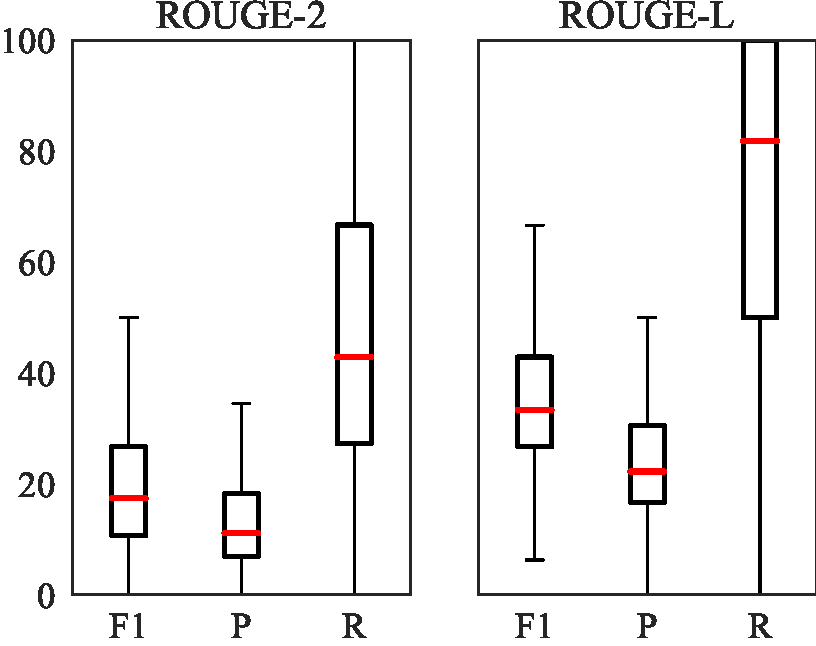
\includegraphics[width=.32\textwidth]{images/thesis/result_boxplots/logsummary_bart-large-cnn-zsl}}%
\hfill{}%
\subfloat[\hadoop{}]{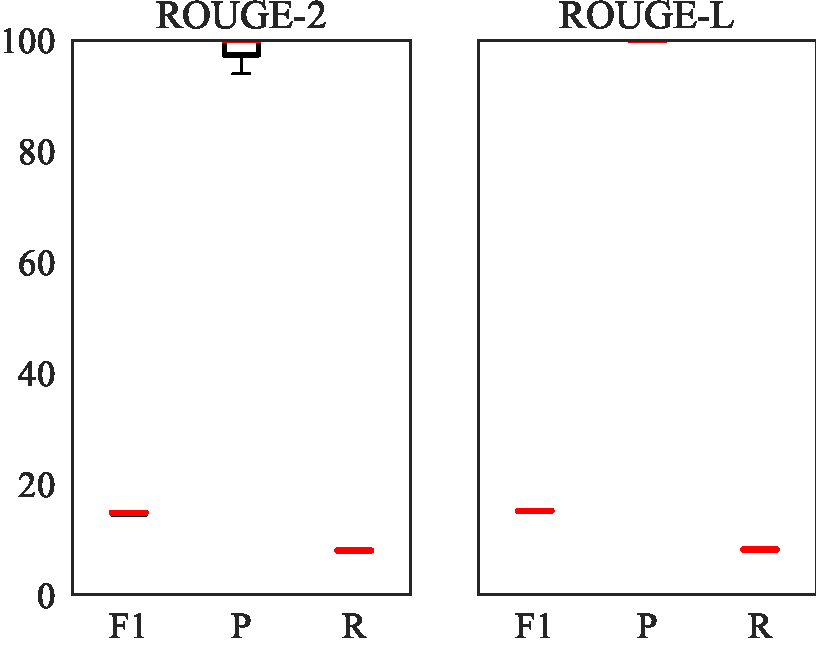
\includegraphics[width=.32\textwidth]{images/thesis/result_boxplots/hadoop_bart-large-cnn-zsl}}%
\hfill{}%
\subfloat[\telco{}]{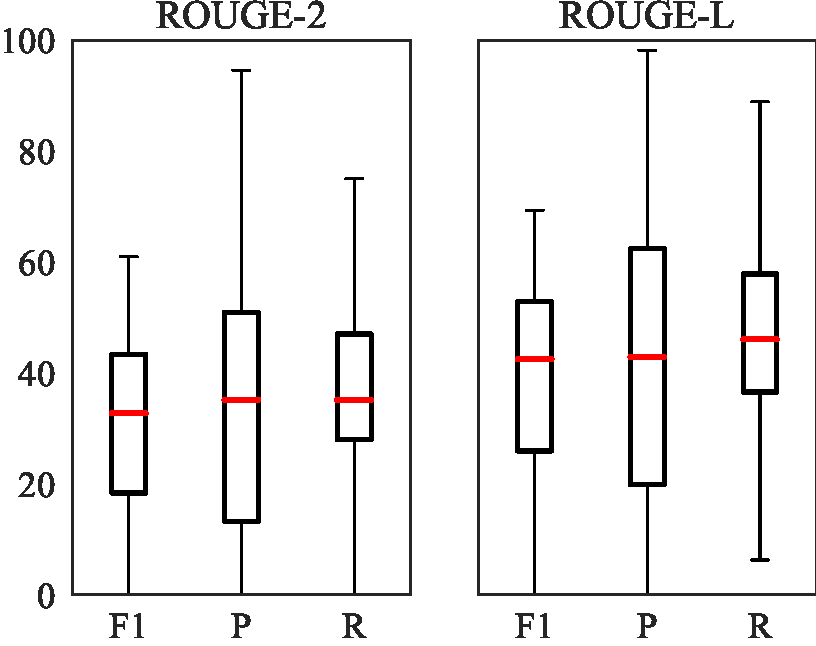
\includegraphics[width=.32\textwidth]{images/thesis/result_boxplots/telcoapp_bart-large-cnn-zsl}}
\caption{Boxplots showing \acs*{rouge} recall, precision and \(F_1\)-scores
of \bart{-CNN} without further fine-tuning (\acs*{zsl}) on all datasets.}
\label{fig:bart_cnn_zsl_all_datasets}
\end{figure}

\begin{figure}[htbp]
\centering
\subfloat[\logsummary{}]{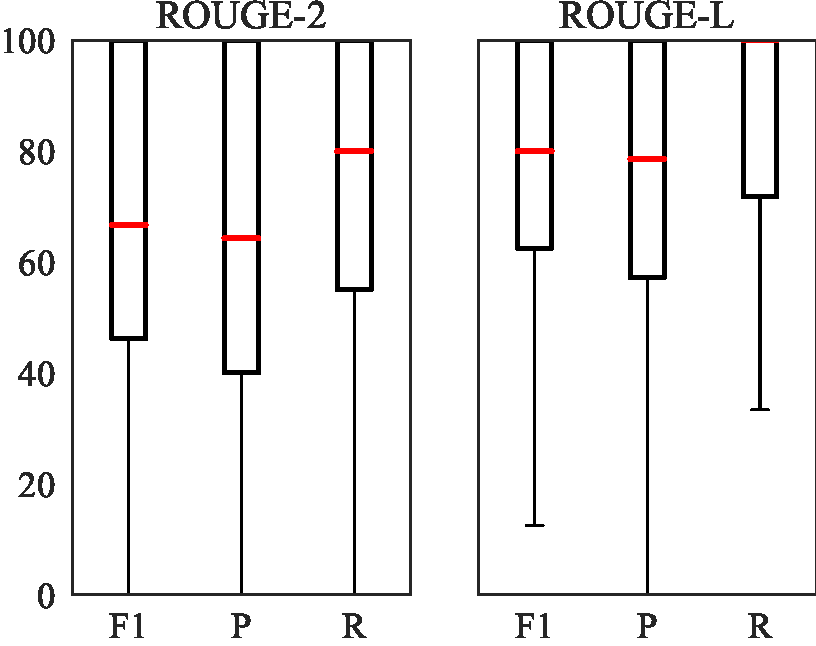
\includegraphics[width=.32\textwidth]{images/thesis/result_boxplots/logsummary_bart-large-cnn}}%
\hfill{}%
\subfloat[\hadoop{}]{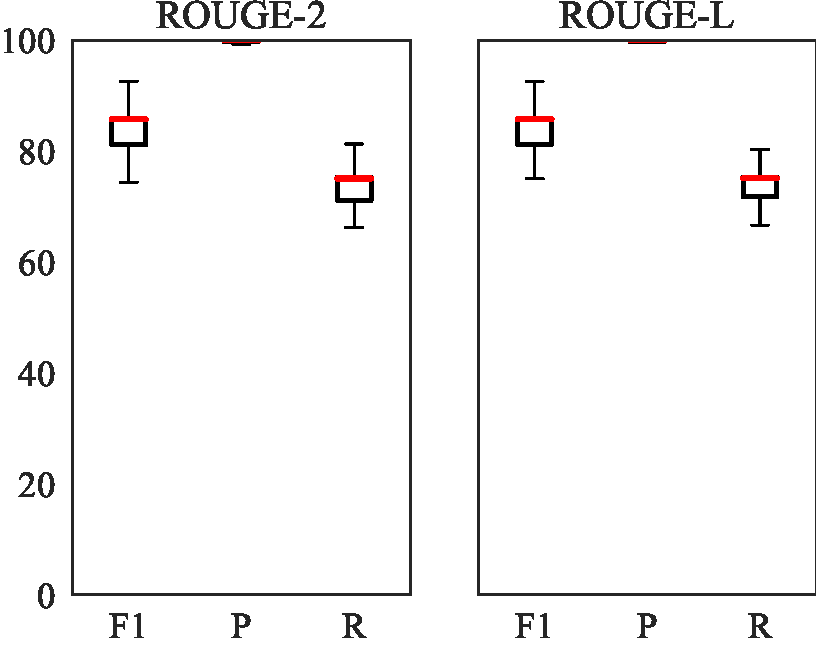
\includegraphics[width=.32\textwidth]{images/thesis/result_boxplots/hadoop_bart-large-cnn}}%
\hfill{}%
\subfloat[\telco{}]{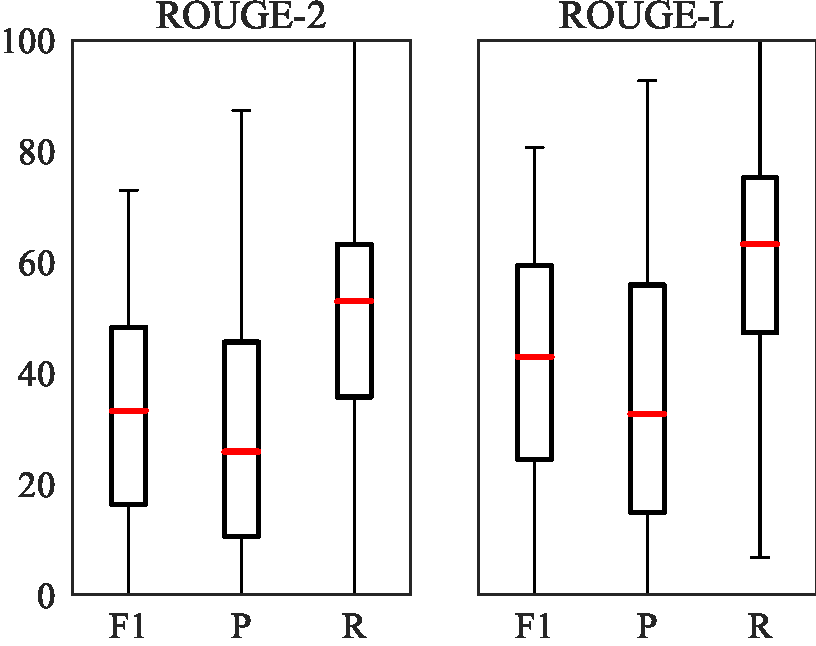
\includegraphics[width=.32\textwidth]{images/thesis/result_boxplots/telcoapp_bart-large-cnn}}
\caption{Boxplots showing \acs*{rouge} recall, precision and \(F_1\)-scores
of \bart{-CNN} with further fine-tuning (\acs*{fsl}) on all datasets.}
\label{fig:bart_cnn_fsl_all_datasets}
\end{figure}

While we previously found that fine-tuning improves performance substantially,
this seems less clear when looking at the BART-model's performance on the \telco{}-dataset.
The \(F_1\) scores remained at almost the same level, though recall is noticeably higher;
at the expense of a equally lower precision.
Unfortunately, it seems that fine-tuning was not able to improve the performance on this dataset,
though it should be noted that the model was able to extract \(49.4\%\)
of the information contained in the reference summary \emph{without} any fine-tuning,
according to the mean summary-level \acs*{rouge}-L recall.
This is while keeping around \(42.3\%\) of the information in the summary relevant,
according to the mean summary-level \acs*{rouge}-L precision.

We do observe however strict improvements on the \hadoop{} and \logsummary{} datasets,
on \hadoop{} mostly due to a substantial improvement in recall.
The results on both datasets seem promising.

However, the \hadoop{}-dataset is actually comprised of logs from 3 failure types,
which are not present in equal proportions, while running one of two different applications.
As the summaries vary in length and form between failure types,
it becomes important to also consider the results for each failure separately.
Thus we report the same metrics as before
in \autoref{fig:bart_cnn_zsl_all_datasets} for  the \ac{zsl} case,
and in \autoref{fig:bart_cnn_fsl_all_datasets} for \ac{fsl}.

\begin{figure}[b]
\centering
\subfloat[Disk full\\\,\clap{\scriptsize{}(15 examples)}]{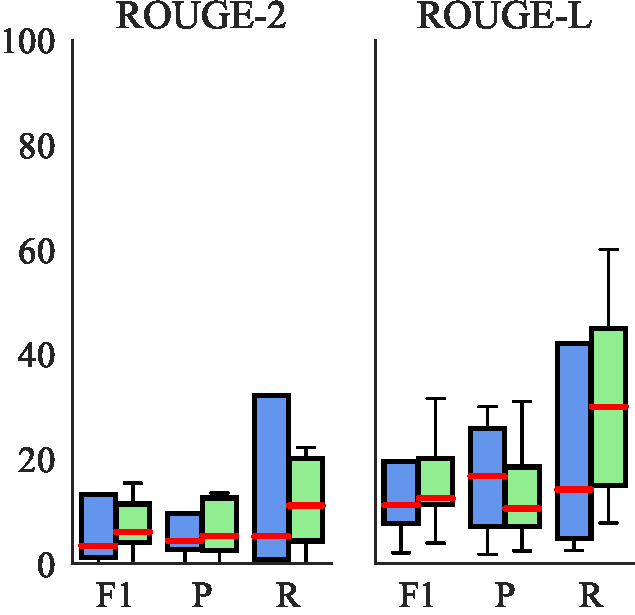
\includegraphics[width=.32\textwidth]{images/thesis/result_boxplots/bart-large-cnn-zsl_disk_full}}%
\hfill{}%
\subfloat[Machine down\\\,\clap{\scriptsize{}(214 examples)}]{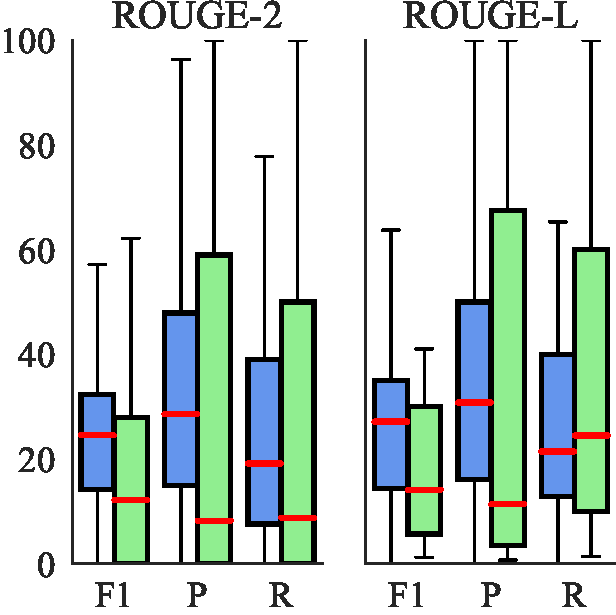
\includegraphics[width=.32\textwidth]{images/thesis/result_boxplots/bart-large-cnn-zsl_machine_down}}%
\hfill{}%
\subfloat[Network disconnection\\\,\clap{\scriptsize (826 examples)}]{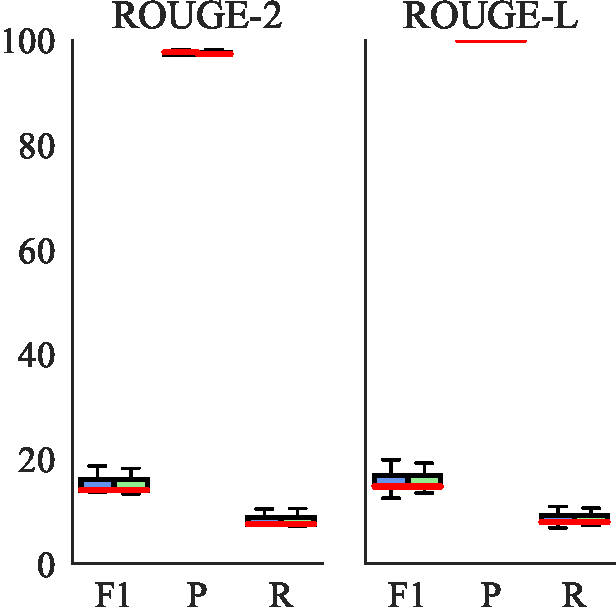
\includegraphics[width=.32\textwidth]{images/thesis/result_boxplots/bart-large-cnn-zsl_network_disconnection}}
\caption[Boxplots showing \acs*{rouge} recall, precision and \(F_1\)-scores
of \bart{-CNN} without further fine-tuning (\acs*{zsl}) on \hadoop{} categorized by failure type and application.]{Boxplots showing \acs*{rouge} recall, precision and \(F_1\)-scores
of \bart{-CNN} without further fine-tuning (\acs*{zsl}) on \hadoop{} categorized by failure type and application (PageRank on the left, WordCount on the right).}
\label{fig:bart_cnn_zsl_hadoop}
\end{figure}

\begin{figure}[t]
\centering
\subfloat[Disk full\\\,\clap{\scriptsize{}(15 examples)}]{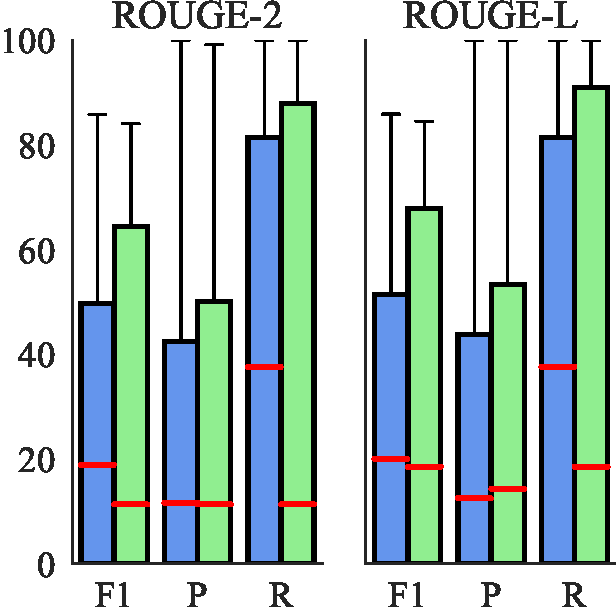
\includegraphics[width=.32\textwidth]{images/thesis/result_boxplots/bart-large-cnn_disk_full}}%
\hfill{}%
\subfloat[Machine down\\\,\clap{\scriptsize{}(214 examples)}]{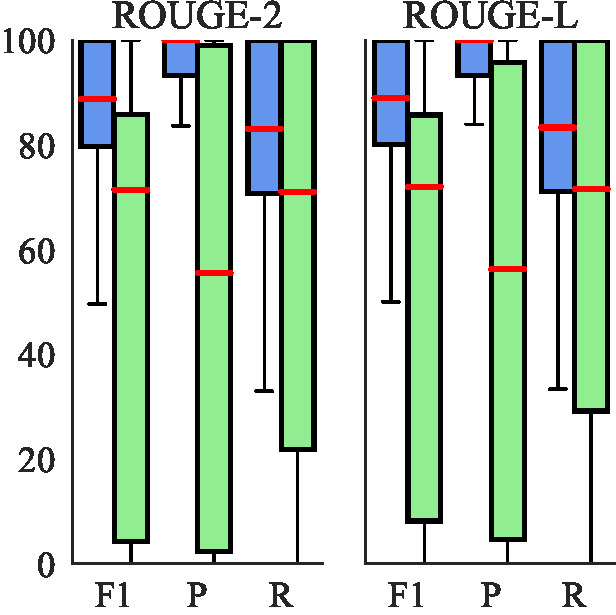
\includegraphics[width=.32\textwidth]{images/thesis/result_boxplots/bart-large-cnn_machine_down}}%
\hfill{}%
\subfloat[Network disconnection\\\,\clap{\scriptsize{}(826 examples)}]{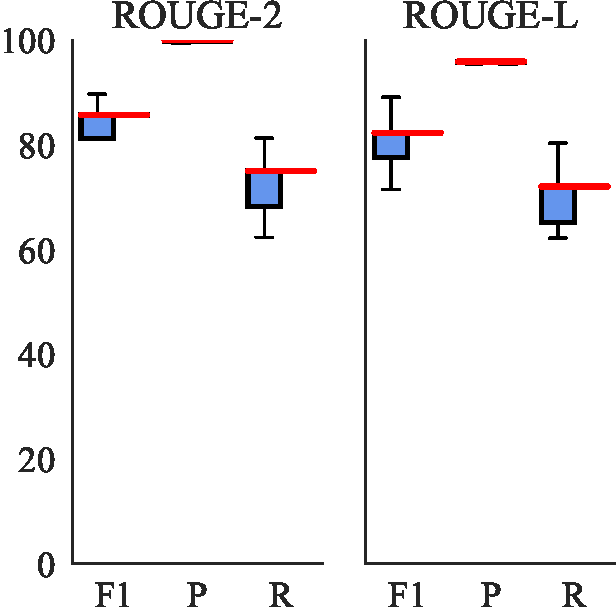
\includegraphics[width=.32\textwidth]{images/thesis/result_boxplots/bart-large-cnn_network_disconnection}}
\caption[Boxplots showing \acs*{rouge} recall, precision and \(F_1\)-scores
of \bart{-CNN} with further fine-tuning (\acs*{fsl}) on \hadoop{} categorized by failure type and application.]{Boxplots showing \acs*{rouge} recall, precision and \(F_1\)-scores
of \bart{-CNN} with further fine-tuning (\acs*{fsl}) on \hadoop{} categorized by failure type and application (PageRank on the left, WordCount on the right).}
\label{fig:bart_cnn_fsl_all_hadoop}
\end{figure}

Now we can see that the \hadoop{}-dataset includes mostly examples from a \emph{network disconnection} failure,
which overshadow the results on the two other failure types.
The continued fine-tuning improved precision \emph{and} recall,
except for the \emph{full disk} failure type where the continued training actually decreased the precision or recall in some cases.

It should be reiterated,
that the training set contained 5 examples for each application on the \emph{full disk} failure,
leaving 11 examples from the WordCount application
and 4 examples from the PageRank application in the test set for this failure type.
Hence we might expect the models to do best in the \ac{fsl} setting here,
as it has trained with a higher proportion of the available examples compared to the other to failure types.
However this is not at all what we observe:
Both precision and recall vary widely and especially for the WordCount application little improvements could be made.
It is not empirically sound to take conclusions concerning the performance difference between the applications on this failure type
due to the imbalanced and low number of test examples available for each application.

An evaluation of the performance on the \emph{machine down} failure is more meaningful,
as the model has only seen 10 examples per application in this dataset.
The test set then contains 181 examples for PageRank and 33 for WordCount.
Again, this is quite imbalanced between applications,
hence why we might expect the model to do better on the WordCount application,
where it has been trained on a greater share of examples.
Instead we observe that the model maintains its preference for the PageRank summaries from the \ac{zsl}-phase.

Regarding this same failure,
for PageRank the model's summaries actually include \(81.1\%\) of the tokens contained in the non-normal log messages
according to the mean summary-level \acs*{rouge}-L recall after pre-training.
On the other hand, the summaries contain \(16.7\%\) tokens not present in the reference summaries
according to the complement of the mean summary-level \acs*{rouge}-L precision.
As such, the model does manage to identify over \(\frac{4}{5}\) of the relevant information,
while keeping the amount of irrelevant information close to \(\frac{1}{6}\).

Though, one-sixth of \emph{factually inconsistent} information
would still be harmful to the quality of the summaries.
Unfortunately \acs*{rouge} is unable to judge the origin or truthiness of the irrelevant portions of the summary.
As such, and to further gain an intuitive understanding of the big variance in performance between the failure types,
we also qualitatively examine one representative example for each failure.

We choose an example whose \ac{fsl}-prediction scores nearest to the median of
summary-level \acs*{rouge}-L \(F_1\) score for each failure type,
to get an idea of the model's average summarization ability.
For comparison we also show the summary in the \ac{zsl} setting,
but omit the input to the model for brevity.

The results are shown in
\autoref{tab:bart_cnn_hadoop_disk_full_example} for the \emph{full disk} failure,
\autoref{tab:bart_cnn_hadoop_machine_down_example} for the \emph{machine down} failure,
and
\autoref{tab:bart_cnn_hadoop_network_disconnection_example} for the \emph{network disconnection} failure.

\begin{table}[htbp]
\centering
\footnotesize
\setlength{\parskip}{1cm}
\begin{tabularx}{\textwidth}{XXX}
\toprule
\textbf{reference summary}
&\textbf{\bart{-CNN} \ac{fsl}}
&\textbf{\bart{-CNN} \ac{zsl}}\\
&\tiny\acs*{rouge}-L \(F_1\): \(18.52\)
&\tiny\acs*{rouge}-L \(F_1\): \(11.88\)\\
\midrule
\tiny\ttfamily\hbadness=10000
Task: attempt\#59489 - exited : DiskChecker: Could not find any valid local directory for out-path

Diagnostics report from attempt\#59489: Error: DiskChecker: Could not find any valid local directory for out-path

Diagnostics report from attempt\#59489: Error: DiskChecker: Could not find any valid local directory for out-path

1 failures on node microsoft.
&
\tiny\ttfamily\hbadness=10000
Diagnostics report from attempt\#83820: Container killed by the ApplicationMaster. Container killed on request. Exit code is 137 Container exited with a non-zero exit code 137

Diagnostics report from attempt\#97248: Container killed by the ApplicationMaster. Container killed on request. Exit code is 137 Container exited with a non-zero exit code 137
&
\tiny\ttfamily\hbadness=10000
Diagnostics report from attempt\#83820: Container killed by the ApplicationMaster. Exit code is 137 Container exited with a non-zero exit code 137. After Scheduling: PendingReds:0 ScheduledMaps:0 ScheduledReds:0 AssignedMaps:3 AssignedReds:1 CompletedMaps:8 CompletedReds:0 ContAlloc:19 ContRel:0 HostLocal:10 RackLocal:8.
\\
\bottomrule
\end{tabularx}
\caption{Representative predictions on a full disk failure of \hadoop{}.}
\label{tab:bart_cnn_hadoop_disk_full_example}
\end{table}

\begin{table}[htbp]
\centering
\footnotesize
\setlength{\parskip}{1cm}
\begin{tabularx}{\textwidth}{XXX}
\toprule
\textbf{reference summary}
&\textbf{\bart{-CNN} \ac{fsl}}
&\textbf{\bart{-CNN} \ac{zsl}}\\
&\tiny\acs*{rouge}-L \(F_1\): \(88.89\)
&\tiny\acs*{rouge}-L \(F_1\): \(22.43\)\\
\midrule
\tiny\ttfamily\hbadness=10000
Retrying connect to server: microsoft. Already tried 15 time(s); maxRetries=45

\textelp{} \textit{(message repeats 4 times with different retry-counts)}
&
\tiny\ttfamily\hbadness=10000
Retrying connect to server: microsoft. Already tried 15 time(s)

maxRetries=45

\textelp{} \textit{(messages repeat 3 times with different retry-counts)}
&
\tiny\ttfamily\hbadness=10000
Retrying connect to server: microsoft. Already tried 15 time(s)

maxRetries=45

Progress of TaskAttempt attempt\#14835 is : 0.23333333

MapCompletionEvents request from attempt\#14835. startIndex 7 maxEvents 10000

\textelp{} \textit{(message repeats 2 times)}
\\
\bottomrule
\end{tabularx}
\caption{Representative predictions on a machine down failure of \hadoop{}.}
\label{tab:bart_cnn_hadoop_machine_down_example}
\end{table}

\begin{table}[htbp]
\centering
\footnotesize
\setlength{\parskip}{1cm}
\begin{tabularx}{\textwidth}{XXX}
\toprule
\textbf{reference summary}
&\textbf{\bart{-CNN} \ac{fsl}}
&\textbf{\bart{-CNN} \ac{zsl}}\\
&\tiny\acs*{rouge}-L \(F_1\): \(82.28\)
&\tiny\acs*{rouge}-L \(F_1\): \(15.09\)\\
\midrule
\tiny\ttfamily\hbadness=10000
Failed to renew lease for NONMAPREDUCE for 1389 seconds. Will retry shortly... NoRouteToHostException: No Route to Host from MININT-FNANLI5remote host \#73234 to msra-sa-41:9000 failed on socket timeout exception: NoRouteToHostException: No route to host: no further information; For more details see: http-URL Caused by: NoRouteToHostException: No route to host: no further information

Address change detected. Old: msra-sa-41remote host \#94343 New: msra-sa-41:9000

\textelp{} \textit{(messages repeat 6 times with incremented timeout)}
&
\tiny\ttfamily\hbadness=10000
Failed to renew lease for NONMAPREDUCE for 1389 seconds. Will retry shortly... NoRouteToHostException: No Route to Host from MININT-FNANLI5remote host \#73234 to msra-sa-41:9000 failed on socket timeout exception: NoRouteToHostException: No route to host: no further information

For more details see: http-URL Caused by: NoRouteToHostException: No route to host: no further information

Address change detected. Old: msra-sa-41remote host \#94343 New: msra-sa-41:9000

\textelp{} \textit{(messages repeat 4 times with incremented timeout)}

Failed to renew lease for NONMAPREDUCE for 1394 seconds. Will retry shortly... NoRouteToHostException: No Route to Host from
&
\tiny\ttfamily\hbadness=10000
Failed to renew lease for NONMAPREDUCE for 1389 seconds. Will retry shortly... NoRouteToHostException: No Route to Host from MININT-FNANLI5remote host \#73234 to msra-sa-41:9000 failed on socket timeout exception: NoRouteToHostException: No route to host: no further information.
\\
\bottomrule
\end{tabularx}
\caption{Representative predictions on a network disconnection failure of \hadoop{}.}
\label{tab:bart_cnn_hadoop_network_disconnection_example}
\end{table}

If we interpret the summaries for the full disk failure in \autoref{tab:bart_cnn_hadoop_disk_full_example},
we notice that the model has learned that messages starting with \verb+Diagnostics report from attempt+ usually are important.
Looking at the reference summary provided in that example, this does seem to be usually the case.
Unfortunately, in this specific case this heuristic did not work out for the model,
because the cancellation of an attempt is actually an benign activity,
and the model failed to include any of the more relevant messages about disk failures.

In the case of the machine down failure in \autoref{tab:bart_cnn_hadoop_network_disconnection_example},
the model missed to include one repetition of the relevant message and would have achieved a perfect score otherwise.

Similarly, for the network disconnection failure in \autoref{tab:bart_cnn_hadoop_network_disconnection_example}
we can actually speculate that the \ac{fsl} model would have correctly continued the message,
however it was cutoff by a maximum length limit we imposed upon the beam-search.
As this is the typical structure of a network disconnection failure,
we can expect that the recall would actually improve on this failure type,
if we had allowed the model to generate longer summaries.
As it maintained a close to perfect precision on this failure until now,
this would probably result in a strict improvement of \(F_1\) scores.

Overall, the model does well in the last two failure types,
where summaries often repeat a message multiple time,
but does worse for the more diverse full disk failure.
On the other hand, this is also where the model has experienced less training.

The \ac{zsl} model performs worse in all examples,
managing to select some of the same messages as the model in the \ac{fsl} setting,
but also including a great portion of irrelevant messages.

Yet, we have to wonder whether this success in caused by the models summarization abilities,
or if the summaries are just too trivial. For the network disconnection failure specifically,
the repeated message which is part of the summary is quite long.
As such they likely represent a majority of the input data.\\
We decide to investigate and calculate the ratio of log messages shared between the model inputs and the reference summaries,
visualizing the results in \autoref{fig:hadoop_summary_document_overlap}.

\begin{figure}[htbp]
\centering
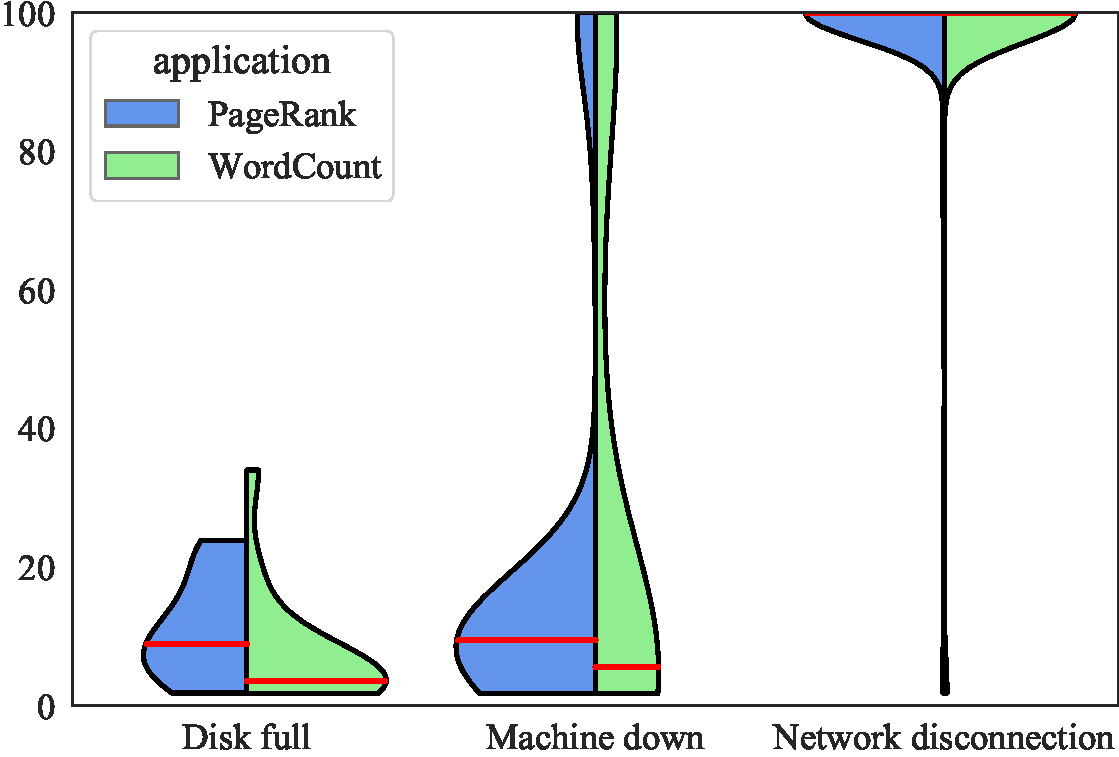
\includegraphics[width=.75\textwidth]{images/thesis/hadoop_curated_summary_document_overlap}
\caption{Violin plot showing the percentage of log messages shared between model inputs and the summaries on \hadoop{}.}
\label{fig:hadoop_summary_document_overlap}
\end{figure}

It is clear now that on the network disconnection failure we do not actually evaluate the model's performance to summarize,
since the input and reference summaries are identical in most cases.
Rather, the \ac{fsl} model as just learned to replicate the relevant message as many times as needed,
while the \ac{zsl} model just selects the first occurrence.
However, the summarization task is meaningful on the other two failure types.
Concerning the machine down failure type, we can now infer a cause for the difference in performance between the logs from the PageRank and WordCount applications:
As indicated by the higher median, the summaries for the PageRank application share more log messages with the input documents.
We assume this is one cause of the higher performance we observe for logs originating during the execution of the PageRank application.

All in all, the example predictions were factually consistent,
including only log messages present in the input data,
but sometimes selecting irrelevant ones.
From manually inspecting other examples,
we conclude that this is the situation in general.

\paragraph{PEGASUS}

Again, we visualize the \acs*{rouge}-2 and summary-level \acs*{rouge}-L recall, precision and \(F_1\)-scores
in \autoref{fig:pegasus_large_zsl_all_datasets} for \pegasus{-Large} under the \ac{zsl} setting.
For \ac{fsl} the results are shown in \autoref{fig:pegasus_large_fsl_all_datasets}.

\begin{figure}[p]
\centering
\subfloat[\logsummary{}]{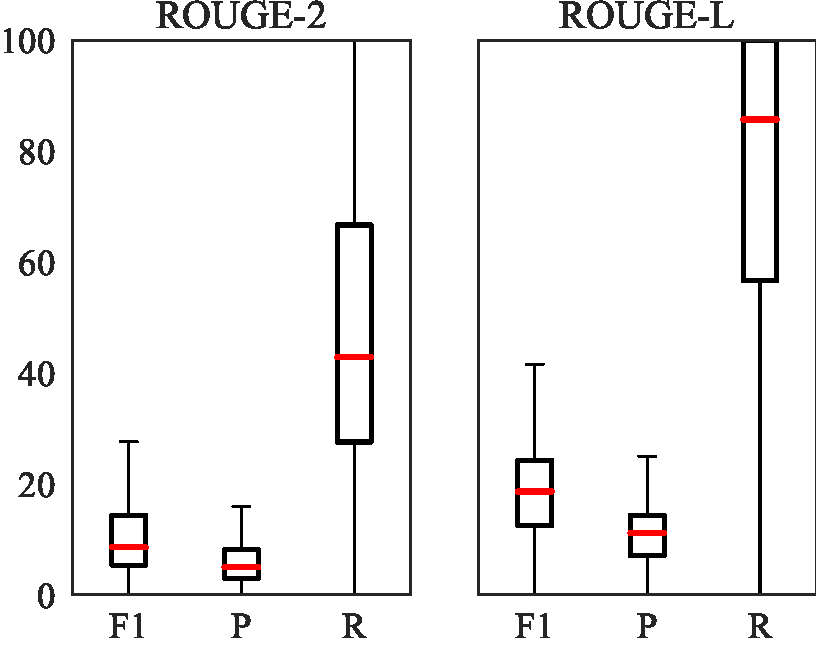
\includegraphics[width=.32\textwidth]{images/thesis/result_boxplots/logsummary_pegasus-large-zsl}}%
\hfill{}%
\subfloat[\hadoop{}]{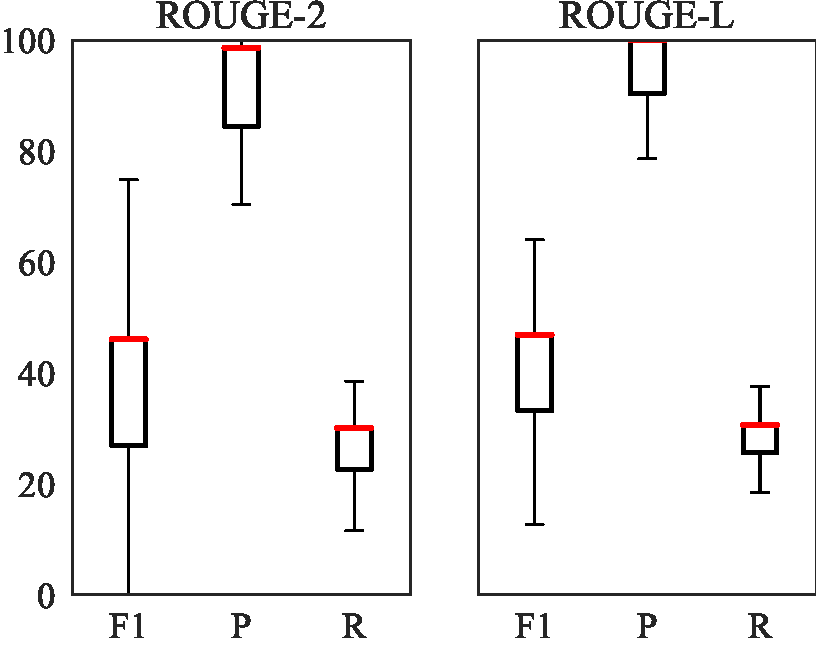
\includegraphics[width=.32\textwidth]{images/thesis/result_boxplots/hadoop_pegasus-large-zsl}}%
\hfill{}%
\subfloat[\telco{}]{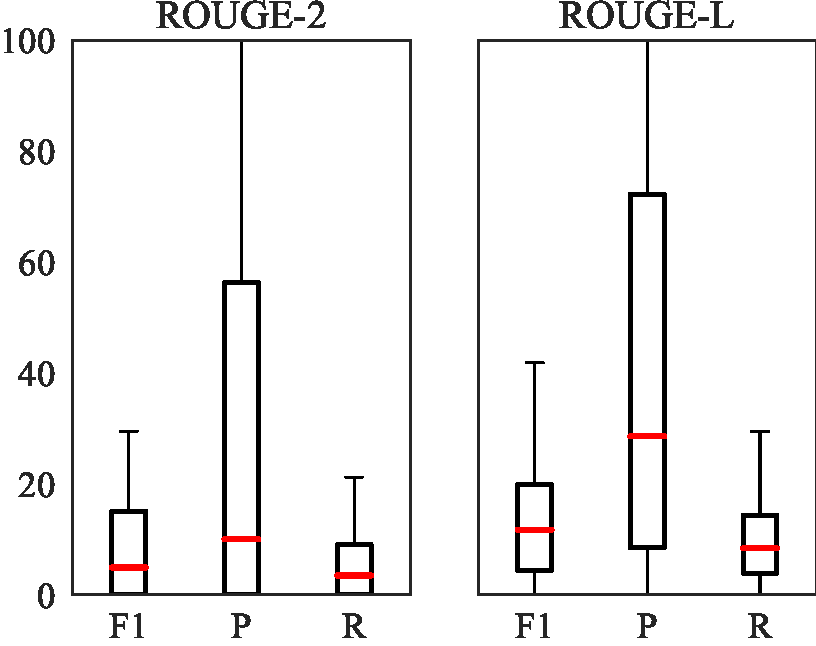
\includegraphics[width=.32\textwidth]{images/thesis/result_boxplots/telcoapp_pegasus-large-zsl}}
\caption{Boxplots showing \acs*{rouge} recall, precision and \(F_1\)-scores
of \pegasus{-Large} without further fine-tuning (\acs*{zsl}) on all datasets.}
\label{fig:pegasus_large_zsl_all_datasets}
\end{figure}

\begin{figure}[p]
\centering
\subfloat[\logsummary{}]{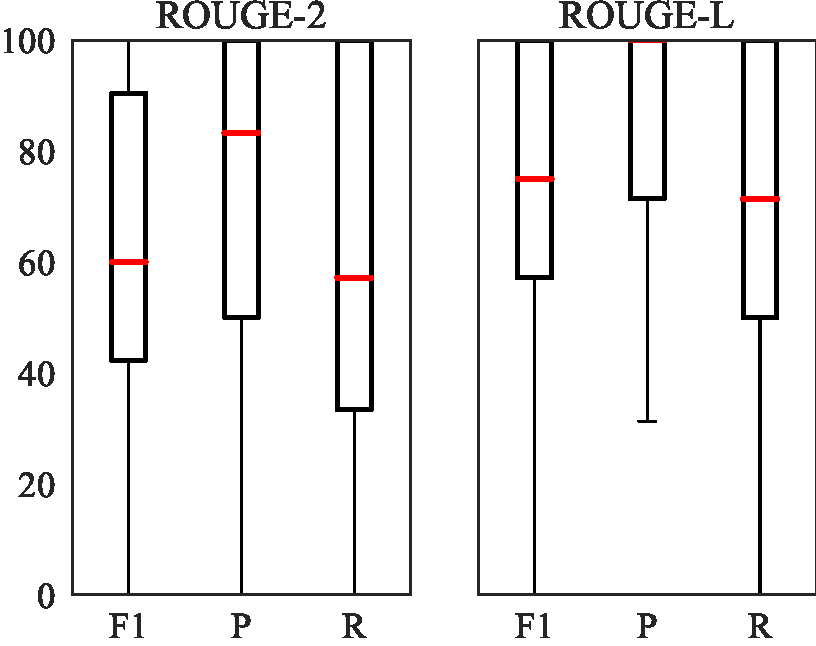
\includegraphics[width=.32\textwidth]{images/thesis/result_boxplots/logsummary_pegasus-large}}%
\hfill{}%
\subfloat[\hadoop{}]{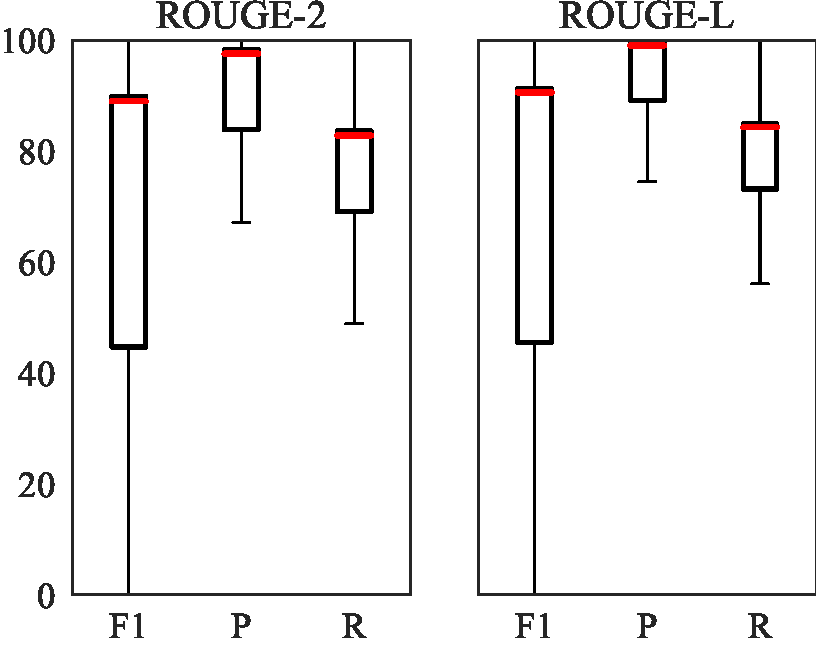
\includegraphics[width=.32\textwidth]{images/thesis/result_boxplots/hadoop_pegasus-large}}%
\hfill{}%
\subfloat[\telco{}]{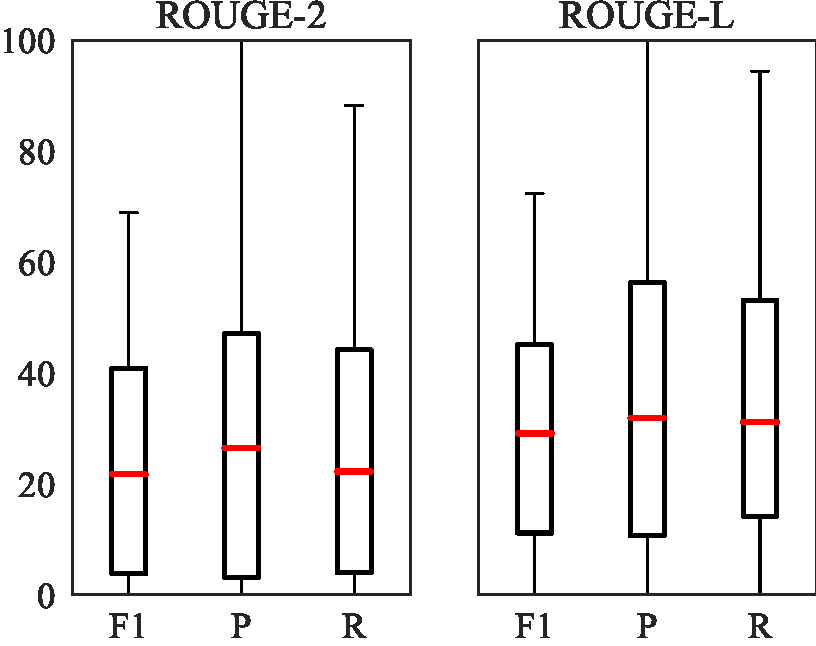
\includegraphics[width=.32\textwidth]{images/thesis/result_boxplots/telcoapp_pegasus-large}}
\caption{Boxplots showing \acs*{rouge} recall, precision and \(F_1\)-scores
of \pegasus{-Large} with further fine-tuning (\acs*{fsl}) on all datasets.}
\label{fig:pegasus_large_fsl_all_datasets}
\end{figure}

The fine-tuning for \pegasus{-Large} actually helped on all datasets, even on \telco{}.
However, one should point out that \bart{-CNN} performed more than twice as good in a \ac{zsl} setting
compared to \pegasus{-Large}, when considering the median \(F_1\)-score for summary-level \acs*{rouge}-L.
Even after fine-tuning this situation does not improve by much.

On the \telco{} dataset we observe that the PEGASUS model manages to achieve higher precision than the BART model in a \ac{fsl} setting,
at the expense of recall.

Finally, on the \hadoop{} dataset the achieved performances vary much more than with \bart{-CNN}.
This remains true when considering the results by failure type,
shown in \autoref{fig:pegasus_large_zsl_hadoop} for the \ac{zsl} case,
and in \autoref{fig:pegasus_large_fsl_hadoop} for \ac{fsl}.

\begin{figure}[htbp]
\centering
\subfloat[Disk full\\\,\clap{\scriptsize{}(15 examples)}]{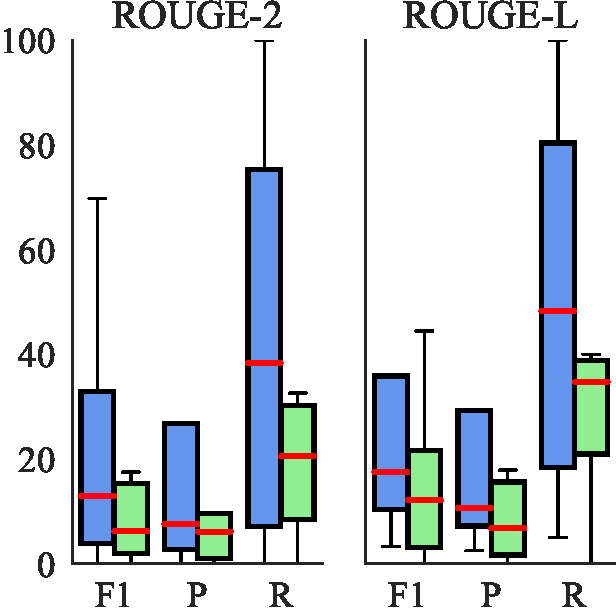
\includegraphics[width=.32\textwidth]{images/thesis/result_boxplots/pegasus-large-zsl_disk_full}}%
\hfill{}%
\subfloat[Machine down\\\,\clap{\scriptsize{}(214 examples)}]{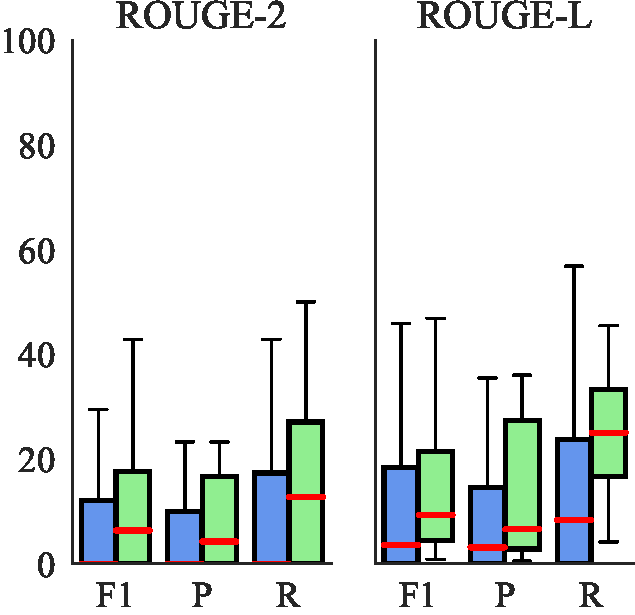
\includegraphics[width=.32\textwidth]{images/thesis/result_boxplots/pegasus-large-zsl_machine_down}}%
\hfill{}%
\subfloat[Network disconnection\\\,\clap{\scriptsize (826 examples)}]{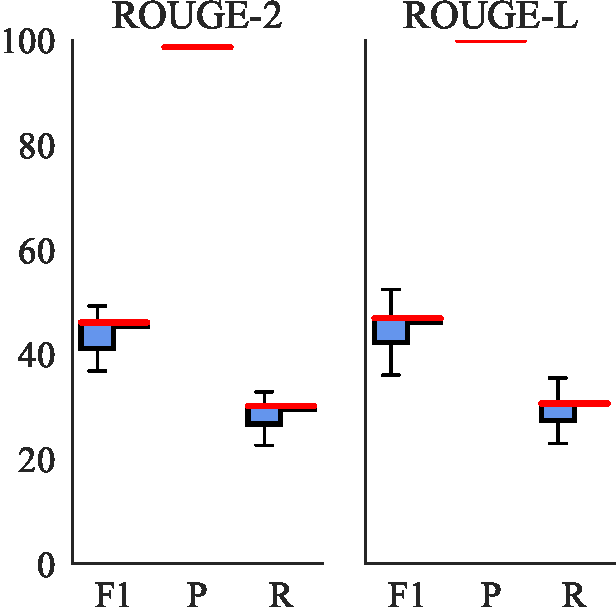
\includegraphics[width=.32\textwidth]{images/thesis/result_boxplots/pegasus-large-zsl_network_disconnection}}
\caption[Boxplots showing \acs*{rouge} recall, precision and \(F_1\)-scores
of \pegasus{-Large} without further fine-tuning (\acs*{zsl}) on \hadoop{} categorized by failure type and application.]{Boxplots showing \acs*{rouge} recall, precision and \(F_1\)-scores
of \pegasus{-Large} without further fine-tuning (\acs*{zsl}) on \hadoop{} categorized by failure type and application (PageRank on the left, WordCount on the right).}
\label{fig:pegasus_large_zsl_hadoop}
\end{figure}

\begin{figure}[htbp]
\centering
\subfloat[Disk full\\\,\clap{\scriptsize{}(15 examples)}]{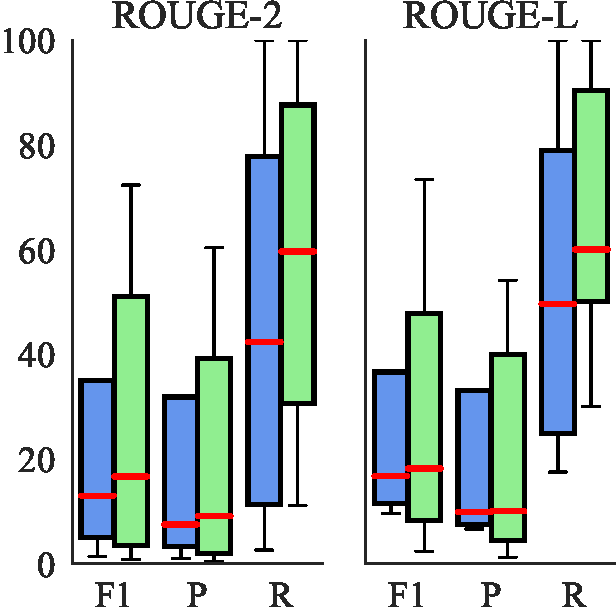
\includegraphics[width=.32\textwidth]{images/thesis/result_boxplots/pegasus-large_disk_full}}%
\hfill{}%
\subfloat[Machine down\\\,\clap{\scriptsize{}(214 examples)}]{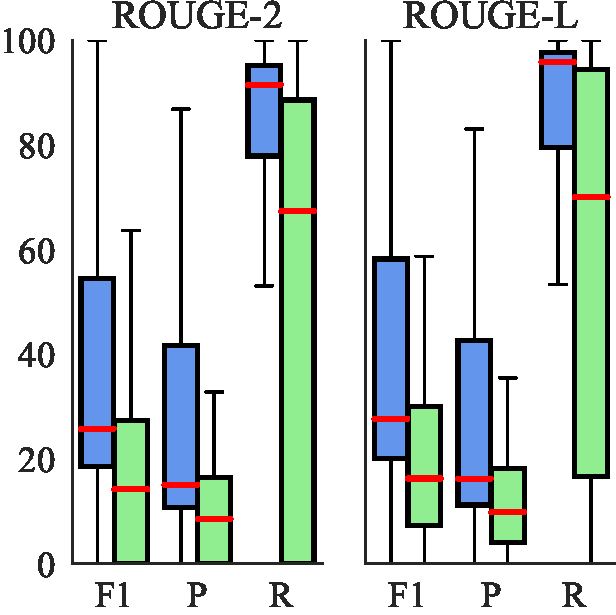
\includegraphics[width=.32\textwidth]{images/thesis/result_boxplots/pegasus-large_machine_down}}%
\hfill{}%
\subfloat[Network disconnection\\\,\clap{\scriptsize{}(826 examples)}]{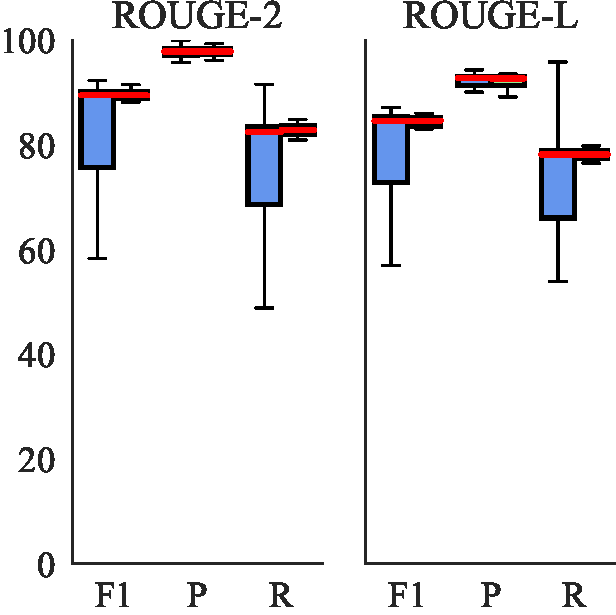
\includegraphics[width=.32\textwidth]{images/thesis/result_boxplots/pegasus-large_network_disconnection}}
\caption[Boxplots showing \acs*{rouge} recall, precision and \(F_1\)-scores
of \pegasus{-Large} with further fine-tuning (\acs*{fsl}) on \hadoop{} categorized by failure type and application.]{Boxplots showing \acs*{rouge} recall, precision and \(F_1\)-scores
of \pegasus{-Large} with further fine-tuning (\acs*{fsl}) on \hadoop{} categorized by failure type and application (PageRank on the left, WordCount on the right).}
\label{fig:pegasus_large_fsl_hadoop}
\end{figure}

Altogether,
\bart{-CNN} outperforms \pegasus{-Large} in all observed settings as can be seen in \autoref{tab:final_models_comparison},
where the best results have been highlighted.
As such we decide to omit any further investigations of the performance of the PEGASUS model for the sake of brevity.

\begin{table}[htbp]
\centering
\footnotesize
\begin{tabular}{rccc}
                          & \multicolumn{3}{c}{\scriptsize{}\bart{-CNN} / \pegasus{-Large}}\\
                          & \h{\logsummary{}}       & \h{\hadoop{}}           & \h{\telco{}}\\
\midrule
\acs*{rouge}-1            & \h{76.3}/72.9           & \h{75.8}/70.4           & \h{40.5}/29.6\\
\acs*{rouge}-2            & \h{66.0}/61.7           & \h{75.6}/68.5           & \h{33.0}/23.7\\
\acs*{rouge}-3            & \h{52.8}/45.9           & \h{75.4}/66.9           & \h{29.2}/21.5\\
\acs*{rouge}-4            & \h{42.0}/33.6           & \h{75.3}/65.4           & \h{26.1}/19.7\\
(sentence) \acs*{rouge}-L & \h{69.7}/67.9           & \h{75.6}/69.4           & \h{37.2}/26.9\\
(summary) \acs*{rouge}-L  & \h{76.3}/72.9           & \h{75.8}/70.3           & \h{40.4}/29.4\\
\end{tabular}
\caption[Mean \acs*{rouge} \(F_1\)-scores of \bart{-CNN} and \pegasus{-Large} in the \acs*{fsl} setting on all datasets.]{Mean \acs*{rouge} \(F_1\)-scores of \bart{-CNN} (left) and \pegasus{-Large} (right) in the \acs*{fsl} setting on all datasets.}
\label{tab:final_models_comparison}
\end{table}

\newpage
\subsection{Discussion}\label{subsec:evaluation_experiment_finetuned_discussion}

We start the discussion of the final results by providing an overview of previous observations:
\begin{itemize}
\item Even fine-tuning on a fraction of the available examples greatly improves performance.
\item Models previously fine-tuned for abstractive summarization (e.g. \pegasus{-BigPatent}) perform poorly in our setting,
      as our datasets are purely extractive.
\item The best models manage to keep summaries factually consistent, by only including segments previously seen in the input data.
\item PEGASUS models fail to adapt to the domain of logs as fast as BART models do.
\item Summarization of logs resulting from a network disconnection failure in \hadoop{} is not meaningful.
      These represent a majority of the examples in this dataset.
      Instead the results on the other two failure types are of greater relevance.
\end{itemize}

Given that PEGASUS outperformed BART on previous summarization datasets and it represents a model with more parameters,
its poor performance in our experiments is somewhat unexpected.
However, the difference between BART and PEGASUS is more pronounced on the XSum dataset,
than the CNN/DailyMail dataset~\parencites{bart}{pegasus}, meaning that PEGASUS is generally better at abstractive summarization.
Since our datasets are highly extractive, PEGASUS' performance improvements may simply be less significant.
Furthermore, we observed that the perplexity of PEGASUS models converges slower than the one of BART models.
As such PEGASUS models may need an increased number of fine-tuning epochs to reach their full potential.

On another note, one problem we frequently observed is a precision/recall-tradeoff:
Optimizing one measure often comes at the cost of lowering the other.
We see this between models originating from differing domains (e.g. the BART variants in \autoref{fig:bart_trial_fsl_logsummary}),
or when comparing the \ac{zsl} \bart{-CNN} model with the \ac{fsl} one on \telco{}.
In the more general setting of information retrieval this is a well-studied problem,
and has been shown to be unavoidable in many situations~\parencite{precision_recall_tradeoff}.

In some situations, it is beneficial to prioritize one measure over the other;
receiving a short but precise description of the most important aspect of a segment of log data is helpful to gain an overview,
but is not sufficient to analyze the causes of a problem.
Conversely, on a longer span of log-data which shows high recall it requires more effort to gain a superficial understanding,
but it can be analyzed more thoroughly.

For \telco{}, even without fine-tuning
\bart{-CNN} was able to capture almost half of the information contained in the reference summary,
but still a majority of the summary does not contain relevant information.
This performance is not good enough to replace manual analysis of the log-data,
but an operator may still consult the model
to get a rough idea of the anomalous log messages before diving deeper into the details,
speeding up the analysis conducted.

The summarization task on the \hadoop{} dataset (and to an extend on the \telco{} dataset as well) could be interpreted as an \emph{anomaly detection} task,
where the model is asked to identify anomalous log messages:
After all, this is essentially the premise of our summarization task based on non-normal log events.

On these types of inputs, the summary length may vary significantly, depending on how many anomalies are present.
Not every failure produces the same amount of anomalous log messages (as can be seen with the \hadoop{}-dataset),
and the model may be asked to investigate normally occurring portions of a log,
where there is not a lot to report on.
It may thus be tricky to find optimal values for the length penalty, affecting a model's performance.

Training a model as a binary classifier (\enquote{Is a given message relevant or not?}) may be better suited for this task than an abstractive \acl{seq2seq} architecture.
One needs not to worry about the model introducing factual inconsistencies, or finding optimal values for the length penalty.
\Acl{seq2seq} architectures still have an advantage over traditional classifiers,
in that they are naturally able to consider the surrounding \emph{context} of a message to judge if it is important or not.

On the other hand, there may also be requirements for summarization similar to that in \logsummary{},
where summarization of benign activity is normal and represents a majority of the data presented to the model.
Here the length of the summaries can be expected to be a stable proportion of the input length,
and sensible values for hyperparameters like the length penalty may be chosen in advance.
We analyze the performance on the \logsummary{} dataset in greater detail in \autoref{sec:evaluation_experiment_logsummary},
however our results suggest that \bart{-CNN} operates well in this kind of setting.

Last but not least, it is arguably not helpful for a human operator to receive a summary
with the same type of log message repeated multiple times,
as is the case in the \hadoop{}-dataset.
As a further preprocessing in the summarization based on \emph{non-normal log events},
log messages could be excluded from a summary
whose log events occur more than once in the reference summary.

Since the model would not be encouraged to repeat the same group of anomalous log messages,
this would result in more concise summaries, and possibly more accurate ones,
because the model has less chances to introduce inconsistencies.
By removing redundancy, the same amount of useful information could be presented to human operators,
while the model would be able to scan over longer portions of the log without running into problems of input limitation.
Shorter summaries also lead to less computation time required for the beam-search.

However, omitting this preprocessing step may be helpful in situations where the dynamic contents of a log message (its parameters)
contains important information and dropping log messages of duplicated event type loses this information.

\paragraph{Conclusion}

We conclude that using models previously fine-tuned for summarization in other domains
does not substantially contribute to better performances.
Instead it seems sufficient to use a pre-trained model and fine-tune it directly on the limited log-data available.
As is perhaps to be expected, summarization of log-data does not seem to have that much in common with other summarization domains.
Although we studied a wide range of previously researched summarization domains,
there may be other summarization datasets where this does not hold true,
especially concerning extractive summarization tasks.
Nevertheless, we suspect any benefits from previous fine-tuning to become less relevant
when fine-tuning is scaled up to larger log summarization datasets.

Overall, the application of pre-trained \ac{nlp} models to log data was a successful proof-of-concept,
however further research is needed to construct better datasets for log summarization.
Models are able to reproduce log data seen in their inputs,
and are able to pick up distinctions between important segments of logs and less important ones.
Our best-performing models still achieve some meaningful performances.
For instance, \bart{-CNN} \acs{fsl} is able to retrieve \(81.1\%\) of the anomalous information
contained in its inputs with high precision when observing the \emph{machine down} failure of the PageRank application (according to summary-level \acs*{rouge}-L).
On the \logsummary{} dataset, \bart{-CNN} \acs{fsl} shows promising results,
reaching a summary-level \acs*{rouge}-L score of \(76.3\) out of a theoretically possible \(100\);
The performance on this dataset is further explored in a later section.

\section{Effects of further Pre-Training on Log-Data}\label{sec:evaluation_experiment_pretraining}

Previous research suggests that further pre-training can significantly improve the performance on later downstream tasks,
especially when data for fine-tuning is not available in larger quantities and the domain a model was trained on differs from the domain it is applied in~\parencites[56-57]{pretraining_study}[8345]{dont_stop_pretraining}.
In this section we thus investigate the effects of further pre-training on the performance in log summarization.

As detailed on \autopageref{subsubsec:approch_experiment_2} we implemented the self-supervised pre-training objective of BART,
and apply it to the \bart{-Base} model.
It is infeasible to pre-train an already fine-tuned BART model such as \bart{-CNN}.
Hence we use the smaller \bart{-Base} baseline model, because pre-training it is faster due to the reduced amount of parameters that are adjusted during training.

We decide to pre-train the model on our largest collection of logs: The logs forming the basis of the \telco{} dataset.
Incidentally, this allows us to examine if pre-training can help to improve the performance on the dataset our models found most challenging.
Additionally, we test whether pre-training is helpful when we later fine-tune the model on a dataset distinct from the one using during pre-training.
As such we also evaluate the models in the \logsummary{} dataset .

\subsection{Experimental Setup}

We evaluate \bart{-Base} in four different settings:
\begin{description}[parsep=0pt,topsep=0pt]
\item[\acf{zsl}]
      The model is directly evaluated on the summarization task without further training.
\item[\acf{fsl}]
      The model is fine-tuned on the summarization task and then evaluated.
\item[\acf{prezsl}]
      The model is pre-trained in a self-supervised manner on the log-data
      and then evaluated on the summarization task without further fine-tuning.
\item[\acf{prefsl}]
      The model pre-trained on the log-data is further fine-tuned on the supervised summarization task and then evaluated.
\end{description}
The \ac{fsl} fine-tuning is conducted in the same manner as described in \autoref{sec:evaluation_experiment_finetuned},
including the same number of steps, batch-sizes and learning rates.

For pre-training we leverage our largest collection of logs: The logs forming the basis of the \telco{} dataset.
The log segments used as the basis of our summaries only represent a fraction of the provided dataset;
As some manual analysis is still needed to identify the relevant segments of the logs where our summarization based on common log events could be applied on,
we only produced reference summaries for a few log files.
Before training, we remove the log files that formed the basis of our summaries,
still leaving us with multiple Gigabytes of log-data.
We do this to prevent the model from later copying inputs it has seen during pre-training.
However, we do not remove logs which originate from similar root causes,
so the logs seen during pre-training are still relevant and similar in style.

During pre-training, we use a comparatively large effective batch size of 8192, similar to the batch sizes used by PEGASUS and BART during pre-training~\parencites{bart}{pegasus}.
The reasoning provided by \citeauthor*{bart} is that previous work demonstrates the effectiveness of large batch sizes during pre-training~\parencite[7875]{bart}.
Analogous to the fine-tuning phase, we use a constant learning rate of \(5 \cdot 10^{-5}\).
We pre-train for 14 epochs, the number of times the model trains on the entire log dataset, resulting in a total of 160 pre-training steps.

Compared to the 500 thousand steps the large BART variants have experienced during their pre-training,
this is a small amount of steps, relatively speaking.
The pre-training is still quite time-intensive for our computing setup, so we were unable to scale up pre-training to much more steps.
However, due to the large batch sizes, the model has actually seen a considerable amount of log data,
and may already employ its knowledge from its previous pre-training.
The role of the continued pre-training is therefore to let the model become acquainted with the log-data,
not to train the model from scratch.

\subsection{Results}

We visualize the cross-entropy loss of \bart{-Base} during pre-training in \autoref{fig:pretraining_loss}.

\begin{figure}[htbp]
\centering
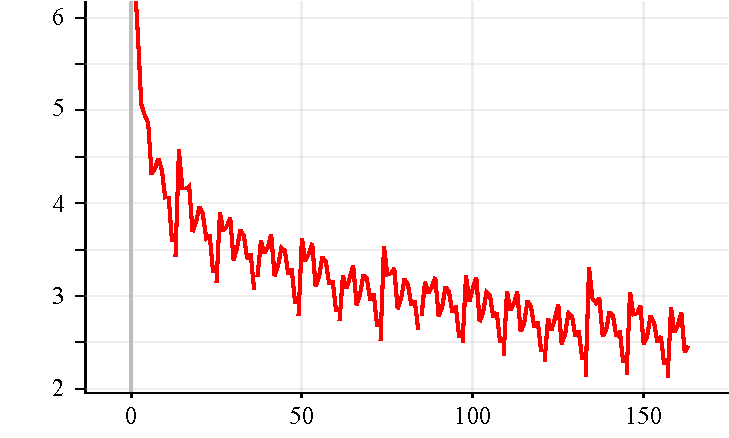
\includegraphics[width=.75\textwidth]{images/thesis/pretraining_loss}
\caption{Cross-entropy loss during the pre-training of \bart{-Base}.}
\label{fig:pretraining_loss}
\end{figure}

Additionally we record the cross-entropy loss on the evaluation data while fine-tuning
and report it in \autoref{fig:telco_finetuning_loss} for \telco{}
and in \autoref{fig:logsummary_finetuning_loss} for \logsummary{}.

\begin{figure}[htbp]
\centering
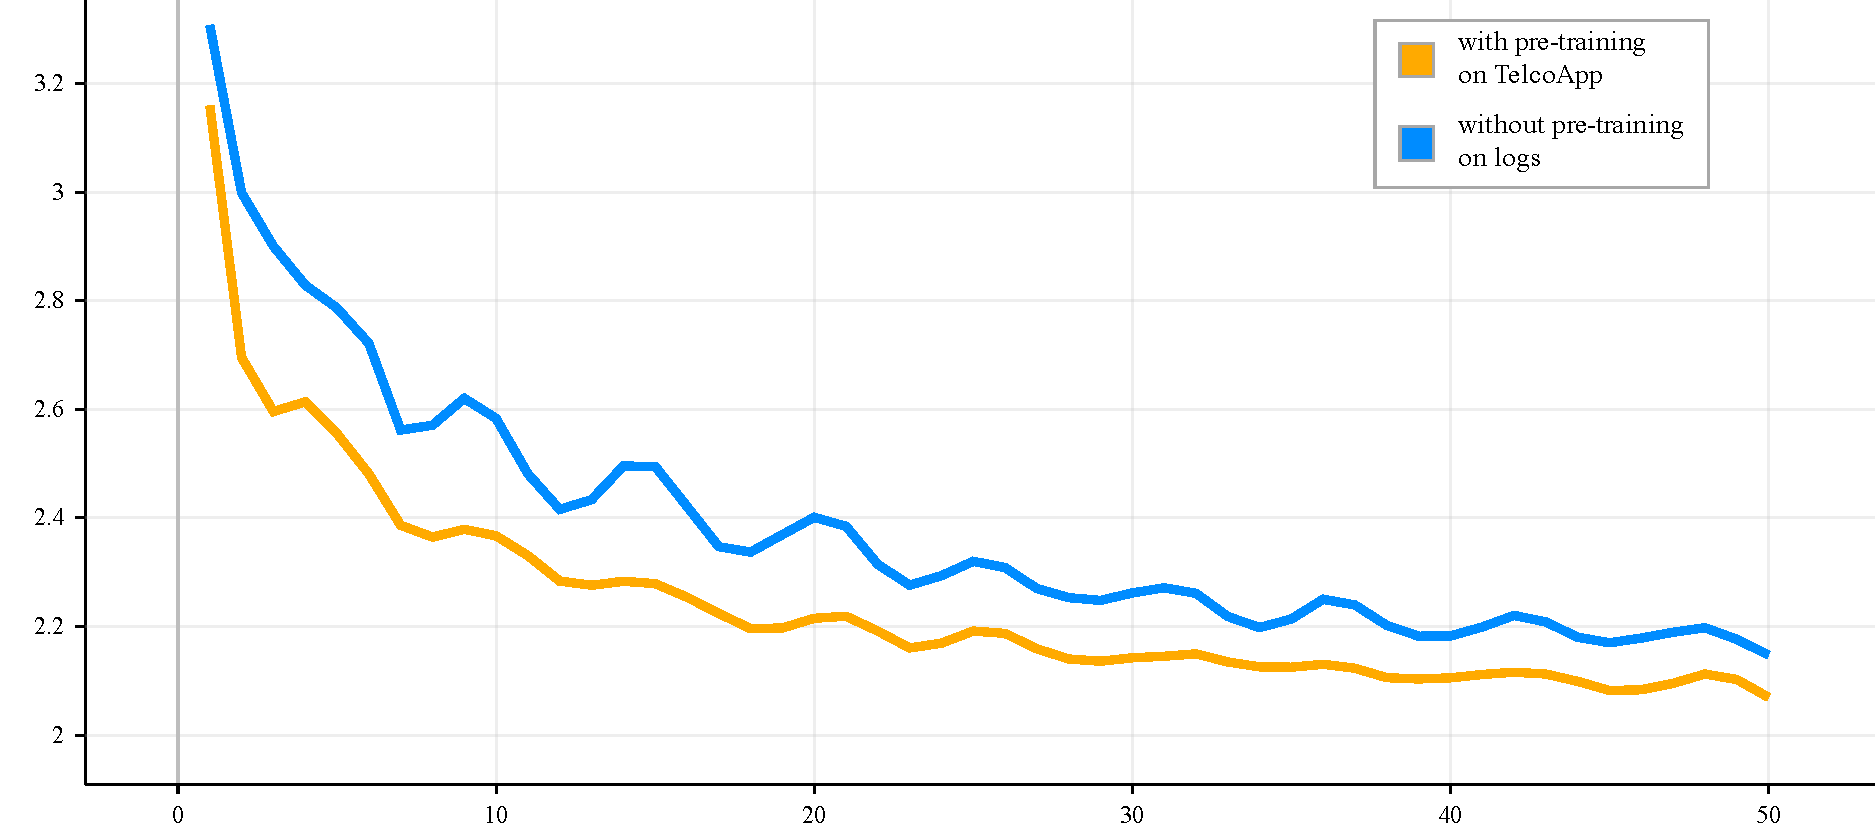
\includegraphics[width=.9\textwidth]{images/thesis/telcoapp_finetuning_loss}
\caption{Cross-entropy loss on the test set during the fine-tuning of \bart{-Base} and the variant pre-trained on \telco{}.}
\label{fig:telco_finetuning_loss}
\end{figure}

\begin{figure}[htbp]
\centering
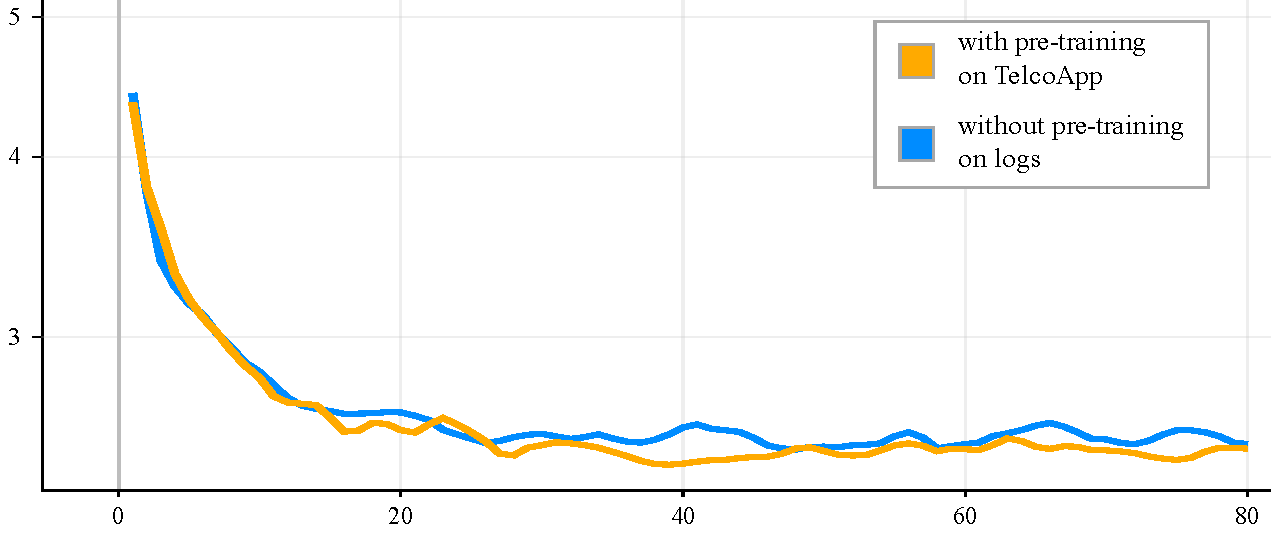
\includegraphics[width=.9\textwidth]{images/thesis/logsummary_finetuning_loss}
\caption{Cross-entropy loss on the test set during fine-tuning of \bart{-Base} and the variant pre-trained on \logsummary{}.}
\label{fig:logsummary_finetuning_loss}
\end{figure}

Finally, we present the results on the summarization datasets
in \autoref{tab:bart_pretrained_comparison_telco} for \telco{}
and in \autoref{tab:bart_pretrained_comparison_logsummary} for \logsummary{}.
The \(F_1\) scores of \acs*{rouge}-1, \acs*{rouge}-2 and sentence-level \acs*{rouge}-L are reported,
and the best results highlighted between the model that experienced further pre-training and the one that did not.
For comparison, we also include the results of \bart{-CNN} from \autoref{sec:evaluation_experiment_finetuned}.

\begin{table}[htbp]
\centering
\footnotesize
\begin{tabular}{lccc}
          & \multicolumn{3}{c}{\scriptsize{}\acs*{rouge}-1 / \acs*{rouge}-2 / \acs*{rouge}-LSent}\\
          & \h{\bart{-Base}}          & \h{\bart{-Base}}               & \h{\bart{-CNN}}\\
          & \scriptsize{}\h{not} pre-trained on log-data
          & \scriptsize{}further pre-trained on \h{\telco{}}
          & \scriptsize{}\h{not} pre-trained on log-data\\
\midrule
\acf{zsl} & 35.2/\h{26.3}/\h{29.2}    & \h{36.4}/25.4/26.1             & 39.2/31.1/33.3\\
\acf{fsl} & 39.4/31.5/35.8            & \h{39.9}/\h{32.1}/\h{35.9}     & 40.5/33.0/37.2\\
\end{tabular}
\caption{Mean \acs*{rouge} \(F_1\)-scores on \telco{} for the different BART variants.}
\label{tab:bart_pretrained_comparison_telco}
\end{table}

\begin{table}[htbp]
\centering
\footnotesize
\begin{tabular}{lccc}
          & \multicolumn{3}{c}{\scriptsize{}\acs*{rouge}-1 / \acs*{rouge}-2 / \acs*{rouge}-LSent}\\
          & \h{\bart{-Base}}          & \h{\bart{-Base}}               & \h{\bart{-CNN}}\\
          & \scriptsize{}\h{not} pre-trained on log-data
          & \scriptsize{}further pre-trained on \h{\telco{}}
          & \scriptsize{}\h{not} pre-trained on log-data\\
\midrule
\acf{zsl} & 25.6/13.8/23.6            & \h{26.8}/\h{14.4}/\h{24.3}     & 35.5/20.6/33.1\\
\acf{fsl} & 76.6/\h{66.4}/\h{71.1}    & \h{76.9}/66.3/70.3             & 76.9/65.9/69.9\\
\end{tabular}
\caption{Mean \acs*{rouge} \(F_1\)-scores of .}
\label{tab:bart_pretrained_comparison_logsummary}
\end{table}

We observe that pre-training alone does improve \ac{zsl} performance a bit,
at least in the \logsummary{} dataset,
but is simplify not enough to create a model able to produce meaningful summaries.
As the model has never been fine-tuned for summarization before, analogous to \bart{-Large},
this is to be expected.
The model has not yet learned that we expect it to write summaries.

All in all, the scores are quite similar after fine-tuning, even when compared to \bart{-CNN}.

\subsection{Discussion}

As can be seen in \autoref{fig:pretraining_loss} the \bart{-Base} model quickly adapts to the new pre-training data,
with the cross-entropy halving within the first 4 epochs.
By the time it reaches around 130 steps, the gains start to stagnate however.
To achieve further significant gains,
we believe it to be likely that the pre-training has to be scaled up to more steps (1000 - 10000).

Furthermore, the cross-entropy fluctuates considerably.
Whenever an epoch of pre-training is finished and a new one starts, the cross-entropy spikes.
This suggests that the log dataset is not homogeneous and the model partly forgets how to handle logs at the beginning of the dataset by the time it finishes an epoch.
The model still is able to consistently lower its cross-entropy overall,
but in the future one may want to shuffle the training data randomly to smooth out the pre-training process.

If we examine the performance of the pre-trained model in the summarization task on \telco{},
we notice that the continued pre-training indeed helped the model better predict the given data;
during fine-tuning it adapts more swiftly and maintains its head-start in cross-entropy even after the fine-tuning is finished.

Unfortunately, the positive impact of continued pre-training on cross-entropy remains confined to the \telco{} dataset.
On \logsummary{}, the pre-training in the domain of log-data did not help \bart{-Base} to make significant performance gains,
neither regarding perplexity nor the \acs*{rouge} metrics.
This is likely due to the difference in style, format and content of various log datasets.
Since \logsummary{} and \telco{} are diverse and distinct from one another,
the model was not able to transfer its newfound knowledge.

From the perspective of cross-entropy, the pre-training was successful for \telco{}.
This improvement in cross-entropy and perplexity however does not translate in a significant difference in summarization performance:
Both the \ac{prefsl} model and the \ac{fsl} baseline show near identical \acs*{rouge}-scores.

Ultimately, continued pre-training did not deliver on the performance improvements we initially expected from it.
We speculate that continued pre-training can still be useful for other tasks than the ones we studied
because the model was able to achieve lower perplexity much faster, even if pre-training did not help on our datasets.

Last but not least,
we remark that after fine-tuning, the base model achieved similar performances compared to the \bart{-CNN} model on both datasets.
To us, this indicates not only that previous training in another summarization dataset is not that relevant to our application
but also that smaller models may be able to achieve similar performances to variants with more parameters.
Since smaller models consume less memory and are faster, both during training and text generation, this is a promising result.

\section{Comparison with the LogSummary framework}\label{sec:evaluation_experiment_logsummary}

Besides introducing a dataset of summarized log-data,
\citeauthor*{log_summary} also introduced their own framework for summarizing logs called \emph{LogSummary}~\parencite{log_summary},
which is explained in greater detail in \autoref{ch:related_work}.

In this section, we aim to compare our results directly with this previous work.
As the LogSummary framework is specifically laid out to only extract parts of any given log messages,
it would perform badly on the two summarization datasets \hadoop{} and \telco{} we introduced ourselves,
where models are expected to reproduce entire log messages.
Therefore we only compare on the \logsummary{} dataset, however we will differentiate between each subdataset as was done in \parencite{log_summary}.

\subsection{Experimental Setup}

We choose our best performing model (\bart{-CNN}) and compare it with the LogSummary framework.

To keep the comparison fair, we need to skip our simplification step from \autoref{subsec:preprocessing},
as the framework works directly on the log messages without needing any simplification.
As such, we take the baseline \bart{-CNN} and fine-tune it on the raw log messages,
otherwise using the same \ac{fsl} setting as in the previous experiment.
To find an optimal length penalty for the beam-search, we again employ an automatic hyperparameter search with 20 trials.\\
We take this as an opportunity to test how helpful our simplification step was for the model,
by comparing the results with the \bart{-CNN} model fine-tuned on the simplified messages.

For the LogSummary framework, we use the results as reported in \parencite{log_summary}.
For the two datasets (Spark and Zookeeper) not included in the original article,
we manually run the LogSummary framework on these datasets and fix any errors encountered.%
\footnote{LogSummary's repository is available at: \url{https://github.com/WeibinMeng/LogSummary}}
This also requires us to manually train two Log2Vec~\parencite{log2vec} models, which are used by the LogSummary framework.%
\footnote{Log2Vec's repository is available at: \url{https://github.com/NetManAIOps/Log2Vec}}
As we could not find any specific information on the amount of data used to train the Log2Vec models in \parencite{log_summary},
we decide to use the \verb+2k.log+-files provided by \parencite{loghub} for the respective datasets,
as this is also the example data used in the Log2Vec repository.

To verify we conducted this process correctly,
we evaluate the LogSummary framework on the HDFS dataset using their pipeline
and receive mean \acs*{rouge}-1 scores of \(54.7\), \(72.1\) and \(45.4\) for \(F_1\), precision and recall respectively.
For the BGL dataset we obtain \(77.4\), \(83.0\) and \(76.1\).
While these do differ from the scores reported in \parencite{log_summary},
they do so only by a small margin of 1 to 5 points.
Therefore we assume we executed the LogSummary framework correctly and proceed to evaluate it on the two new datasets.

For this experiment only, we use a different implementation of the \acs*{rouge} metric, namely the one used by the LogSummary framework%
\footnote{That implementation is available at \url{https://github.com/pltrdy/rouge}.}, to keep the comparison fair.

\subsection{Results}

Following \parencite{log_summary}, we primarily investigate values of the \acs*{rouge}-1 metric:
The reasoning for comparing only the \acs*{rouge}-1 values provided by \citeauthor*{log_summary}
is that the different authors of each reference summary may have written words and phrases in different succession,
ranking extracted segments by different priorities.
The results are shown in \autoref{tab:comparison_rouge1_logsummary} with the best results on each subdataset highlighted.

The results for the LogSummary framework are for the whole dataset,
while the results of our model are calculated on the test set only.
Since 95 out of 100 examples in each subdataset are in the test set,
the results should still be comparable.

\begin{table}[htbp]
\centering
\footnotesize
\begin{threeparttable}
\begin{tabular}{l@{\qquad}c@{\qquad}c}
                    & \multicolumn{2}{c}{\scriptsize{}\(F_1\) / precision / recall}\\
                    & \h{LogSummary framework}            & \h{\bart{-CNN} \acs{fsl}} (ours)\\
\midrule
BGL                 & \h{72.5}/\h{81.5}/70.3\tnote{*}     & 71.9/72.8/\h{75.3}\\
HDFS                & 53.8/75.9/43.2\tnote{*}             & \h{77.2}/\h{80.2}/\h{75.5}\\
HPC                 & 84.0/81.9/\h{91.1}\tnote{*}         & \h{84.2}/\h{82.8}/88.5\\
Proxifier           & 86.4/87.9/85.7\tnote{*}             & \h{93.1}/\h{99.1}/\h{89.8}\\
Spark               & 59.4/68.9/53.1\tnote{\(\dagger\)}   & \h{79.5}/\h{78.2}/\h{83.8}\\
Zookeeper           & 50.7/58.9/46.0\tnote{\(\dagger\)}   & \h{74.1}/\h{73.6}/\h{79.5}\\
\midrule
average             & 67.8/75.8/64.9                      & \h{80.0}/\h{81.1}/\h{82.1}\\
\bottomrule
\end{tabular}
\begin{tablenotes}
\item[*] Scores as reported by \parencite{log_summary}.
\item[\(\dagger\)] Scores as identified by us from running the framework manually.
\end{tablenotes}
\caption{Mean \acs*{rouge}-\(1\) \(F_1\), precision and recall on the subdatasets of \logsummary{}.}
\label{tab:comparison_rouge1_logsummary}
\end{threeparttable}
\end{table}

We also report the sentence-level \acs*{rouge}-L scores for our approach:
In \autoref{tab:comparison_preprocessing_logsummary} we display the performance of our \bart{-CNN} model on each subdataset of \logsummary{},
and provide the results of the \bart{-CNN} fine-tuned on the simplified messages from \autoref{sec:evaluation_experiment_finetuned} for comparison.

Sentence-level \acs*{rouge}-L provides a measure to evaluate how much information overlap there is between the model generated summary and human-written references,
additionally estimating the model's ability to preserve the order of extracted segments.
Thus we can also assess how well the model can prioritize segments from the subjective ordering assigned to them by the authors of the summaries.

\begin{table}[htbp]
\centering
\footnotesize
\begin{tabular}{l@{\qquad}c@{\qquad}c}
                    & \multicolumn{2}{c}{\scriptsize{}\(F_1\) / precision / recall}\\
                    & \h{simplified messages} & \h{regular messages}\\
\midrule
BGL                 & 59.0/51.8/\h{76.9}      & \h{67.8}/\h{68.4}/71.3\\
HDFS                & 69.3/67.6/\h{73.3}      & \h{69.4}/\h{71.9}/67.9\\
HPC                 & 75.6/71.7/\h{86.0}      & \h{81.1}/\h{79.7}/85.4\\
Proxifier           & \h{95.0}/97.8/\h{93.2}  & 92.2/\h{98.0}/89.1\\
Spark               & \h{68.3}/64.5/\h{75.8}  & 67.0/\h{65.9}/70.5\\
Zookeeper           & \h{62.7}/60.0/\h{68.6}  & 61.5/\h{61.0}/66.3\\
\midrule
average             & 71.6/68.9/\h{79.0}      & \h{73.1}/\h{74.1}/75.1\\
\bottomrule
\end{tabular}
\caption{Mean sentence-level \acs*{rouge}-\(L\) \(F_1\), precision and recall of the fine-tuned \bart{-CNN} models on the subdatasets of \logsummary{}.}
\label{tab:comparison_preprocessing_logsummary}
\end{table}

\subsection{Discussion}

\paragraph{Evaluation of our text simplification during preprocessing}

First, we briefly examine how \bart{-CNN} handles the log-data without using our simplifications;
To our surprise the model performs well, even surpassing the average performance of our previous \bart{-CNN} model using the simplified messages.
The model operating on the raw messages manages to achieve higher precision, only slightly falling of on recall.

However, any direct comparisons should be taken with a grain of salt:
The length penalty the hyperparameter search found for \bart{-CNN} operating on the raw messages encourages shorter summaries than the one for the previous model,
likely being a major cause in the precision/recall-tradeoff we observe.

Still, on the HPC dataset both models achieve almost the same recall, but the model operating on raw messages is more precise.
At the very least, this indicates that there are situations where our simplification step is not helpful.
Further still, at least on the \logsummary{} dataset, the simplification step is likely not a major factor in increasing a model's performance:
After further fine-tuning, \bart{-CNN} is able to summarize raw log messages well enough.

While this means that our simplification step may have been unnecessary,
the possibility that pre-trained \ac{nlp} models may not require a simplification step
based on error-prone regular expressions is actually very promising.

The necessity of simplification may change on datasets including more complex patterns;
we believe it to be likely that simplifying long patterns is still important,
like java stack traces or long file-paths present in the \hadoop{} and \telco{} datasets.
These passages are especially long and contain little important information, displacing more important context.
Altogether though, our simplification step can likely be scaled down without negatively impacting model performance.

\paragraph{Comparison with previous work}

In general, the \bart{-CNN} fine-tuned on raw messages performs comparatively well.
On the BGL dataset, the \(F_1\)-scores are similar, but the summarization framework is more precise.
The contrary is true on the HPC dataset, where \bart{-CNN} is more precise.
On all other remaining datasets, \bart{-CNN} strictly outperforms the previous work by at least \(7\) points regarding the \(F_1\) measure.
Overall, we achieve improved \acs*{rouge}-1 \(F_1\) scores of \(12\) points on average.

Of course, risk of overfitting is present when using deep learning methods.
As the LogSummary framework makes use of unsupervised learning algorithms, it is not affected by this problem.
However, the vocabulary overlap of summaries between training data and test data
is the lowest for the \logsummary{} dataset across all studied datasets
(see \autoref{tab:training_test_vocab_overlap} on \autopageref{tab:training_test_vocab_overlap}).
We do not believe the improved performance of \bart{-CNN} can be explained solely on the basis of overfitting.

Still, we previously only reported the overall vocabulary overlap of summaries,
but there may be substantial differences between the subdatasets of \logsummary{}.
Thus we also report the overlap for each subdataset in \autoref{tab:logsummary_subdatasets_vocab_overlap}.

\begin{table}[htbp]
\centering
\footnotesize
\begin{tabular}{cccccc}
BGL                                 & HDFS                         & HPC &
Proxifier                           & Spark                        & ZooKeeper\\
\midrule
\(\frac{17}{139} \approx 12.230\%\) & \(\frac{10}{25} = 40.000\%\) & \(\frac{26}{66} \approx 39.394\%\) &
\(\frac{17}{22}  \approx 77.273\%\) & \(\frac{20}{61} = 32.787\%\) & \(\frac{22}{72} \approx 30.556\%\)
\end{tabular}
\caption{Ratio of words common between summaries in the respective training and test sets for all subdatasets of \logsummary{}.}
\label{tab:logsummary_subdatasets_vocab_overlap}
\end{table}

Here we see a more diverse picture:
The BGL dataset certainly brings down the average vocabulary overlap between training and test set.
As the summaries on HDFS and Proxifier are less varied in their vocabulary, both in relative and absolute terms,
it is possible that \bart{-CNN} overfits on these datasets.
However, the same model still performs well on the other more diverse datasets,
showing that it is capable of applying its knowledge even on inputs different from its training data.

As opposed to the LogSummary framework, which required a separate Log2Vec model for each subdataset to achieve peak performance,
we trained \bart{-CNN} on all six datasets simultaneously.
Our results suggest that \bart{-CNN} is applicable even in situations
where logs are generated from heterogeneous subsystems with different logging styles.

Last but not least, if we compare \acs*{rouge}-1 to the sentence-level \acs*{rouge}-L for \bart{-CNN},
we observe that the reduction in recall and precision is not drastic, both falling by only 7 points.
This means that \bart{-CNN} was able to mostly imitate the style and subjective structure of the human-written summaries.
We speculate the model can thus also be adapted to other extractive summary styles wished for in practical applications.

All in all, we showed that pre-trained \ac{nlp} models can effectively summarize the contents of log-data,
even with minimal fine-tuning required.
As a \ac{seq2seq} architecture \bart{-CNN} not only outperforms previous work, but is also more flexible by design.

\section{Threats to Validity}\label{sec:threats_to_validity}

As a conclusion to this chapter, we discuss some aspects regarding the validity of our results and conclusions.

\paragraph{Sensitivity to hyperparameters}

The hyperparameters of the beam-search greatly influence the performance of our models.
Previous research confirms this finding,
as \citeauthor*{solving_length_problem} show that machine translation systems are sensitive to the length penalty used
and that different tasks and datasets require different penalties~\parencite[9]{solving_length_problem}.

Finding optimal values is challenging;
The differences observed between the transformer models in our experiments
could in part be caused by suboptimal values for these generation parameters.
We tried to mitigate this in our experiments by using automatic hyperparameter searches
and consulting multiple perspectives (including examining perplexity, which is unaffected by these parameters) to select the best-performing models.
Yet, we cannot fully exclude that some of our findings are influenced by suboptimal hyperparameters,
especially when the differences between performances is small, as was the case for the BART variants in \autoref{sec:evaluation_experiment_finetuned}
or when we examined the effects of pre-training in \autoref{sec:evaluation_experiment_pretraining}.

\paragraph{Problems of \acs*{rouge} as a measure of quality}

Ever since the publication of the \acs*{rouge} metrics, several shortcomings have been pointed out by the academic community:
\begin{itemize}
\item \Acs*{rouge} is unaware of synonyms and expects summaries to closely match the reference summaries~\parencite{rouge2}.
\item In general, \acs*{rouge} only judges the overlap in vocabulary and longer text segments,
      but cannot judge fluency and factual consistency.
      These qualities need to be judged separately, for instance during trials with human judges~\parencite[546]{summarization_critical_evaluation}.
\item Surveys with human judges suggest \acs*{rouge} may be better fit for evaluating extractive models than abstractive models.
      For past model architectures \citeauthor*{summarization_critical_evaluation}
      investigated the correlation of \acs*{rouge}-scores to human judgments of quality:\\
      When considering extractive summaries only, \acs*{rouge}-scores were moderately correlated to human judgments of relevance, fluency, comprehensibility and factual coherence;
      such correlations remain less clear-cut for abstractive summaries~\parencite[545-546]{summarization_critical_evaluation}.
\end{itemize}

Since abstractive models create novel text sequences,
they may have a higher tendency to introduce factual inconsistencies~\parencite[546]{summarization_critical_evaluation},
which \acs*{rouge} cannot judge.
However, from manual inspection of the generated summaries,
we generally observe that the summaries closely follow an extractive style in our case,
not including novel sequences of words.
As our datasets are purely extractive, they encourage this behavior.

We believe this to be beneficial to the applicability of \acs*{rouge} to measure the quality of summaries on our datasets,
since many of the problems described above are directed towards comparing texts that are syntactically different,
but have the same semantic contents.
As both the generated summaries and the reference summaries closely follow the style of the inputs, this should be less of a concern.

\paragraph{Biases in logs}

In the past, summarization models trained on news articles showed a significant bias for the first three sentences of an article.
This has been attributed to a layout bias in journalism where the first parts of an article usually contain more important information~\parencite[544-546]{summarization_critical_evaluation}.
Thus \emph{Lead-3}, selecting the first three sentences of an article, performs well as a heuristical summary for news articles.

Lead-3 as a heuristic has next to no meaning in the context of log-data,
because messages in logs roughly follow a chronological order and are not ordered by significance.
However, there may be other biases in the data that could be used influence performance and should be accounted for.
A few examples come to mind:
\begin{itemize}
\item The setup operations executed at the startup of a system are likely to produce less important log-entries.
      If a model received only inputs that started at the beginning of a log,
      it may learn to ignore the first share of its input.

      On the \hadoop{} dataset it is the case that some of the model inputs start at the beginning of a log,
      where the startup operations happen,
      however the dataset also contains many input documents that start at other portions of a log.
\item Similarly, due to the way we selected the relevant portions of log-data we use as inputs on the \telco{} dataset,
      some of the model inputs necessarily start with log messages that are deemed important by the summarization task based on common log events.
      In these cases it may be advisable to perturb the inputs by including additional log messages at the beginning.
\item Each logging system may exhibit their own biases, with certain formats representing more important messages.
      Consider for example messages starting with \texttt{Diagnostics report from attempt} in the \hadoop{} dataset.
      As we saw in \autoref{tab:bart_cnn_hadoop_disk_full_example} on \autopageref{tab:bart_cnn_hadoop_disk_full_example} these usually represent anomalous messages,
      but not in all cases.
      Operators may find such messages useful in order to identify problems, but they may facilitate overfitting \ac{nlp} models.
\item While there are many lists of \emph{stop words}, which represent words that are less likely to convey important semantic information,
      it is unclear if these apply well to application logs.%
      \footnote{See \url{https://github.com/igorbrigadir/stopwords} for an overview of different stop word lists.}
      Words present in stop word lists are often ignored when evaluating a model using a metric.
      For example, \acs*{rouge} can optionally omit such words when evaluating the quality of a summary.
\item Log-entries often contain metadata such as severity-levels (error, debug, \ldots).
      We suspect errors and warnings may contain a significantly greater share of important information than the average log-entry.
      Related to this assumption, in the past system maintainers used basic keyword searches
      (e.g. searching for words like \emph{failure} or \emph{warning})
      to identify problematic log-lines~\parencite[307-308]{not_basic_keyword_search}.
\item Another potentially important metadata is the software component where the log message originated from.
      Some components will produce more important messages than others,
      because they play different roles in the operation of the system.
      It is possible that components issuing few messages are more likely to write important messages,
      because they represent software execution paths seldomly followed.
\end{itemize}
To avoid such biases and improve their generality, our models did not receive any metadata as inputs.
Still, our models could still be susceptible to the other biases mentioned and further biases not considered in these examples.

On the whole, biases present in log-data are not well researched, even though they are an important aspect influencing the performance and generality of models.
In other summarization datasets, like CNN/DailyMail and XSum, such biases are well-researched and accounted for during the design and evaluation of a model.
Consider for instance the removal of duplicated trigrams employed by BART on the CNN/DailyMail dataset,
which past research has shown to be beneficial~\parencites{bart}{beam_search_duplicate_ngram_removal}:
In other summarization datasets that contain repetitions (like BigPatent~\parencite{bigpatent}) this may be detrimental to the model's performance,
but it is actually helpful here.

\paragraph{Threat to universality}

One actuality we frequently observed during our experiments is that logs can be quite diverse:
\begin{itemize}
\item Logs originating from different systems may use dissimilar vocabularies
      and show less overlap than other previously researched summarization domains.
      As can be seen in \autoref{fig:datasets_vocab_overlap} on \autopageref{fig:datasets_vocab_overlap},
      the datasets from the news domain show a much larger overlap in frequently used words than logs do.
      Further still, logs share little vocabulary with common summarization datasets in general.
\item Logs vary in degree of correct use of capitalization and punctuation,
      meaning that there is no perfect choice for a separator between log messages concerning the pre-trained models investigated.
\item As seen in \autoref{tab:logsummary_subdatasets_vocab_overlap} on \autoref{tab:logsummary_subdatasets_vocab_overlap},
      even by randomly sampling only 5 out of 100 examples for training,
      one can get widely different overlaps in vocabulary for training and test sets,
      on logs originating from different systems.
      Some systems show multifaceted use of different words, while others consist of only a few different log events,
      making it easy to accidentally overfit models on these datasets.
\item Different summarization tasks are applicable to different log datasets.
      We presented the conditions in which we believe our summarization tasks to identify meaningful log events,
      that can be used as the basis for reference summaries,
      yet the nature of the resulting summaries is quite different.
      Summaries based on \emph{common log events} are by nature quite homogeneous when only considering a single root cause,
      while summaries based on \emph{non-normal log events} can be more diverse.

      Both our proposed summarization tasks are \emph{failure-oriented},
      as they require a failure to be present to be applicable,
      but they make use of different assumptions inspired from the log datasets they were applied on.
\item Even logs originating from the same system can be very different,
      as we observed on the \hadoop{} dataset:
      During some failures a group of message is periodically written to the log, leading to large log files,
      which consist of mostly redundant information.
      Other failures only produce small amounts of more diverse anomalous messages, reducing the overall redundancy of the log.
\end{itemize}
This diversity is part of what makes summarization on log-data challenging.
Even worse, it means that our models and summarization tasks may not be applicable to logs from other systems.

\emph{Log summarization} cannot be understood as a singular task,
rather requirements for summaries will vary from system to system.
Even for the human-written summaries in \logsummary{} which all follow a similar style,
the model's performance varies between log segments from different systems.
Our findings may not apply to other log datasets.

In practice, this means that a model should be fine-tuned on each specific dataset it is used on in order to achieve peak performance.
Thankfully,
tuning a pre-trained transformer model with only a few examples can be enough to improve performance and achieve useful results,
as we have demonstrated in our experiments.
Additionally, a single model may be able to handle logs from heterogeneous systems, as our results in the \logsummary{} dataset suggest.

\paragraph{Lack of user studies}

As the idea of textual log summarization is relatively young,
none of the datasets we employ have previously been studied in the context of a user study.
While \citeauthor*{log_analysis} previously found that presenting a condensed representation of log-data to users
can greatly speed up their ability to analyze said data~\parencite{log_analysis},
it is not possible for us to determine if the same is true for the summaries studied by us.

On the \logsummary{} dataset, the summaries are human-written, implying at least a basic degree of quality.
However, on the other two datasets we employed our own summarization tasks,
which construct reference summaries using semi-automatic means.
While we presented several arguments why we believe our summarization tasks to produce informative summaries,
it is still unclear whether system experts would find the resulting reference summaries valuable.


\chapter{Related Work}\label{ch:related_work}

\acresetall

% Related work.
% Present state of research and applied solutions concerning the different aspects relevant to the thesis.
% Discuss differences and similarities to other solutions to the given tackled problem.
% Approximately 5 to 8 pages.

Published research in the context of log summarization is sparse;
however, more generally, log analysis is an active field of research,
with literature presening and demonstrating the effectiveness of
different approaches to gaining insights from logs.

\paragraph{Log analysis}

One fascinating application of log analysis is
in the context of Computer Security, where it can present an important tool to
detect and comprehend attacks on \ac{it} infrastructures.
Systems such as HOLMES or HERCULE try to reconstruct the attack and detect different stages present in cyberattacks:
Starting from the infiltration of the attacker into the system,
the attacker gaining a foothold and escalating their privileges,
up to the collection and extraction of sensitive information and potential cleanup operations.

The HOLMES~\parencite{holmes} system detects ongoing attacks in real-time
by correlating different system events that are extracted from logs,
then using databases of common attack principles and causality rules to differentiate benign activities
from an attack and present a high-level view of the attack in the form of a graph.
For an event or action to be part of the attack,
there must be dependencies between it and suspicious activities from other attack phases.

HERCULE~\parencite{hercule} is based on the observation
that attack-related events are highly correlated and dependent on each other
but are usually not related to other benign activities.
They build a graph of events, connecting log-entries through a multi-edge, denoting a set of predetermined binary features,
like accesses to the same files and web resources, occurrence within a fixed time window, or requests directed at the same remote hosts.
They then apply a \acl{ml} algorithm to collapse the multi-edged graph to a weighted graph
and use community detection to identify communities of related activities.
From these, communities of log-entries containing suspicious activities
are identified as potential attacks and presented to the user.

However, attack detection and reconstruction are only one possible use case where the investigation of log-data proves helpful.
Log analysis is also widely-employed in \ac{it} operations more generally,
not only related to attack detection and reconstruction~\parencite{log_analysis}.
Similar to the reconstruction of an attack tracing anomalous events,
automated \ac{rca} tries to identify the root-cause of a failure and any intermediate steps leading up to the failure.

\citeauthor*{fes_cluster_logs} present a system which facilitates \ac{rca} in log-data.
They identify sequences of log events that frequently occur in the log,
cluster different sequences by the number of events they share,
and construct a dependency graph of related log events
by comparing the chronological order of the events in each cluster.
Given a set of log events that indicate the presence of a failure,
their approach identifies possible causes for these events by tracing the dependencies in the graph.
Ultimately, this dependency graph is presented to a system expert,
who can use the graph to perform an in-depth investigation of the root-cause~\parencite{fes_cluster_logs}.

All these systems have in common that they present an overview of the problem
(as a graph of related events) to a human operator.
This is done to communicate the details of the problem, speed up the understanding of the problem and potential solutions~\parencites{holmes}{hercule},
but also to facilitate further investigations~\parencite{fes_cluster_logs}.
These dependency graphs can be interpreted as \emph{visual} summaries involving log-data of the studied problems.

We believe \emph{textual} summarization models, such as the ones presented by us,
could in the future enhance such visual summaries of log-data by further summarizing groups of log events,
further lowering the effor required to swiftly form a genral understanding of the detected problem.

\paragraph{Transformer-based approaches to log analysis}

One of the first uses of transformer-based models for log analysis was presented by
\citeauthor{logsy} with their NuLog and Logsy architectures.
\emph{NuLog}~\parencite{nulog} represents a self-supervised algorithm for learning log templates and is hence a log parser.
The key idea is to use \ac{mlm} to mask random words in a log message and
instruct a transformer-based language model to predict the missing word.
If the model guesses the word correctly, it is not a dynamic parameter and hence part of the template.
NuLog outperforms Drain~\parencite{drain} and other previously studied log parsers in parsing accuracy,
but also provides a numeric representation (\emph{embeddings}) for each log message.

These numeric embeddings encode a log message as a whole and thus represent the semantic content of each message.
If combined with a supervised binary classifier, this can yield a model for log-based \emph{anomaly detection},
a log analysis task where one tries to identify which log-entries are not the result of a normal execution environment~\parencite{nulog}.
Additionally, an unsupervised anomaly detection model is presented,
which is based on the number of correctly predicted missing words in each log message:
The assumption is that NuLog will not be able to predict the missing words in anomalous messages as well as in normal ones.

Likewise, anomaly detection is the task where the \emph{Logsy}~\parencite{logsy} model was applied to.
The idea is to produce numerical embeddings where normal log messages are close to each other
while anomalous log messages are more distant.
A spherical learning objective is used to train the model
to place normal log messages close to the center of a sphere
and other messages at large distances from this center point.
This hypersphere is part of the same dimensional space as the embedding vectors,
with the center point defined as 0.
%An \emph{anomaly score} between 0 and 1, proportional to the embedding's Euclidean distance from the center,
%is calculated and used in the spherical loss function.
The embedding's Euclidean distance from the center is then used as the \emph{anomaly score} of a log message.
In combination with a threshold \(\varepsilon\), this distance is used to classify the log message;
Embeddings inside the hypersphere with radius \(\varepsilon\) are classified as normal while all other embeddings are not.

During training, the model is presented log messages from the target system it is later applied on,
and auxiliary log messages originating from different openly accessible log datasets.
The messages from the target system are assumed to be mostly normal,
while the auxiliary messages are anomalous by definition, because they do not originate from that system.
Logsy can thus be trained as a supervised classifier, although the data from the target system does not need detailed labeling.
Overall, with unsupervised training on one-fifth of the log
Logsy achieves a recall of \(90\%\) while maintaining a precision of \(26\%\) on the BGL dataset,
which is the most challenging among the 3 different previously studied log datasets.
With the inclusion of \(2.1\%\) labeled training data from the BGL target, the precision improves drastically to \(89\%\),
although the recall slightly decreases to \(72\%\).

On the \hadoop{}-dataset our models could be interpreted as models for anomaly detection,
though we did not evaluate them as such, because they generate arbitrary text.
Hence we are not directly able to measure the overlap in terms of log-entries,
although in practice the models usually reproduced the input log messages exactly,
barring the correct separation between distinct log messages.
However, from the examples we have seen with the full disk failure in the \hadoop{} dataset,
even after supervised fine-tuning, our models may struggle to compete with the high precision and recall of Logsy.

\Ac{seq2seq} models suffer from the problem that the expected outputs in an anomaly detection task can widely vary in length,
making it challenging to find adequate hyperparameters.
Though, these architectures still have an advantage over traditional classifiers,
in that they are naturally able to consider the surrounding \emph{context} of a message to judge if it is important or not,
while classifiers usually work on a line-by-line basis.
This makes it possible for \ac{seq2seq} models to judge, if a log-entry is anomalous in a given context
(e.g. it is anomalous for a network disconnection to happen during regular system operation,
but it is a routine status indication when a device is reconnected to another network as a result of a user-request),
however the usefulness of this depends on the granularity of the presented logs and the existence of appropriate datasets.
If the log-data is too fine-grained and contains interleaving messages from widely different components,
the context of a log message is not that meaningful, especially considering the input size limitations of current transformer models.

\citeauthor{language_models_logging} undertake a study with different language models
(including the transformer-based encoder BERT~\parencite{bert}) on log-data
and use the model's internal embeddings for log anomaly detection~\parencite{language_models_logging}.

They find that embeddings produced by models pre-trained on log-data are more useful for anomaly detection
than when pre-trained on general-purpose text.
However, they find that pre-training BERT on log-data alone does not consistently outperform
the original BERT-model trained on large corpora of natural language texts.
Furthermore, introducing more diverse log-data during pre-training can actually degrade the embeddings' quality.

As opposed to \citeauthor*{language_models_logging}, we followed the advice from \parencite{dont_stop_pretraining}
and did not pre-train a model from scratch:
Even after previous training on general-purpose text,
we observe that further pre-training transformer models on log-data can lower the cross-entropy loss on downstream tasks.
Unfortunately this did not improve the summarization performance in our applications.

Nevertheless, our results from fine-tuning alone,
suggest that even general-purpose transformer models possess some knowledge transferable to the domain of log analysis.

\paragraph{Summarization of logs}

In the context of \emph{visual} log summarization
\citeauthor{logassist} introduced their \enquote{log analysis IDE} \emph{LogAssist}~\parencite{logassist},
which summarizes the information contained in logs and displays a condensed but expandable view to the user,
which is 75.2\% to 93.9\% smaller than the raw logs~\parencite[7]{logassist}.\\
LogAssist constructs workflows from logs, which group multiple related log-entries matching program-flow.
Logs are first parsed into log events using Drain~\parencite{drain},
then grouped by an ID (e.g. a thread-ID) and time-difference.
Finally, redundant event sequences are condensed using \(n\)-gram modeling~\parencite[3-4]{logassist}.
During a user study with 19 participants, they find that
\textcquote[10-11]{logassist}{LogAssist provides, on average, a 42\% improvement in
log analysis speed when compared to performing the same analysis on raw logs alone},
thus demonstrating the need for effective tools to present log-data in a concise way to human operators.

Contrary to our approach,
LogAssist does not aim to generate a textual summary that includes important information from the logs
but instead aims to provide users with a compact representation of logs that can be easily explored.
We believe the \(n\)-gram modeling used to simplify redundant event sequences in their work
could also be effectively applied as a preprocessing step for textual summarization,
helping to produce condensed summaries in situations where important log events
are duplicated many times such as in the \hadoop{}-dataset.

\paragraph{Textual summarization of logs}

\citeauthor{log_summary} apply existing concepts of \ac{nlp}
in their open-access framework \emph{LogSummary}~\parencite{log_summary}
to create textual summaries of log-data and are to our knowledge the first to do so in the context of a scientific publication.

Furthermore they introduce \emph{LogIE},
an information extraction framework for logs that is an integral part of LogSummary;
LogIE combines log templates, a rule-based system and an information extraction framework \emph{OpenIE}
to extract entity-relationship tuples from log messages.~\parencite[4]{log_summary}

The rule-based system first extracts entity-value pairs using commonly occurring patterns in log-data,
such as separator characters like colons between key-value pairs.
Hence it would extract the entity-relationship triples (\verb+Severity+, \verb+is+, \verb+HIGH+)
and (\verb+Reason+, \verb+is+, \verb+NetworkException+) from the log message:
\begin{verbatim}
Error transferring transaction to PersistanceManager!
Will not retry transfer. Severity: HIGH, Reason=NetworkException
\end{verbatim}
Now OpenIE is applied to the remaining part of the message to extract further
tuples of entities, events and their relations, like (\verb+Error+, \verb+transferring+, \verb+transaction+) and (\verb+Will not retry+, \verb+transfer+).

LogSummary then leverages previous techniques to produce vector embeddings for each tuple and ranks them using TextRank~\parencite{textrank};
the top-\(k\) tuples are selected as the summary.

As we focus mainly on the application of pre-trained transformer models on log-data
as opposed to creating a comprehensive framework for summarizing logs,
LogSummary address some additional challenges with log summarization that we did not consider:
\begin{enumerate}
\item \emph{Accurate summaries:} As LogSummary is entirely an extractive summarization framework,
      it does not suffer from some of the problems laid out in \autoref{sec:threats_to_validity};
      Our abstractive models possess the ability to generate arbitrary text not present in the input documents,
      but with that comes the challenge of keeping factual consistency.

      LogSummary is less likely to write a factually inconsistent summary
      as summaries are entirely made up of text segments present in the input data.
\item \emph{High throughput requirements:} Large-scale distributed systems can generate over 500 thousand~\parencites[126]{hdfs_dataset}[125]{logpai_logparser_benchmarks}
      or even 120 million~\parencites[1250]{cloud_diag} log-entries per hour.
      As such, depending on the use case,
      it may be necessary for log summarization methods to be able to process large amounts of log-data.

      While LogIE can process several thousand lines of logs per second on a server \ac{cpu},
      our models require several seconds or minutes to generate a summary for hundreds of log-entries on two deep-learning \acp{gpu}.
      According to benchmarks conducted by HuggingFace transformer-based models may even run between 13 to 23 times slower on a \ac{cpu}.%
      \footnote{\accessurl{https://medium.com/huggingface/benchmarking-transformers-pytorch-and-tensorflow-e2917fb891c2}{06.04.2022}}

      Due to the self-attention mechanism, computation time scales quadratically with respect to input-size for transformer models~\parencite[6]{transformer}.
      Furthermore, the computation time of the beam-search employed for generating text from a model's predictions scales with respect to the length of the text to generate~\parencite[5]{beam_search}.
      In situations where relations between distant log-entries is less important, throughput can hence be significantly improved
      by feeding models smaller portions of log-data at a time or asking for shorter summaries.

      Numerous efforts exist to make transformer-based more time-efficient,
      ranging from optimizations on \acp{cpu} halving computation times~\parencite{transformers_cpu_optimization},
      using mixed precision for training and interference on \acp{gpu}
      benefiting from higher throughput of operations~\parencite{nvidia_mixed_precision}
      or approximating the self-attention mechanism at the core of transformers in a computationally more efficient way~\parencites{bigbird}{nystroemformer}.
      Moreover, previous research found that smaller models may be trained to achieve similar results as larger versions~\parencites{distilbert}.

      On the other hand, LogSummary uses TextRank to rank triples, which actually also exhibits
      quadratic time complexity with respect to input size when used on a complete graph,%
      % NOTE: Could not find good source for PageRank's complexity.
      \footnote{A complete graph of \(n\) nodes is known to have \(\binom{n}{2} = \frac{n \cdot (n - 1)}{2}\) edges,
      while the PageRank-based ranking method is known to have a time complexity of
      \(\mathcal{O}(n + e)\) for a graph with \(n\) nodes and \(e\) edges.
      It follows that \(\mathcal{O}(n + \binom{n}{2}) = \mathcal{O}(\binom{n}{2}) = \mathcal{O}(n \cdot (n - 1)) = \mathcal{O}(n^2)\) is the complexity on a complete graph.}
      as is the case with LogSummary.
      We hypothesize that LogSummary also slows down when scaled up to longer input data.

      Ultimately, we do not expect transformer models to be faster than conventional algorithms in the near future.
\item \emph{Prioritization of important messages:} Our proposed summarization tasks
      discourage from changeing the order of events in the summary.
      However, LogSummary explicitly approximates the importance of each summarized entry and
      thus is able to construct summaries beginning with the most critical segments first.
\item \emph{Removing redundancy in log-data:} Logs often contain multiple repetitions of similar log messages;
      if one such message is part of the summary, other similar log messages may not be as important.
      Our proposed summarization tasks do not remove redundant log-messages from summaries.\\
      We notice this problem with the \hadoop{}-dataset,
      where the disconnection from the network causes the repetition of the same group of log-entries over and over again,
      leading to highly repetitive and unnecessarily long summaries.

      LogSummary addresses this by simply removing duplicated entity-relationship tuples,
      preventing repetition in summaries.
\item \emph{Summarization within log messages:} By only extracting entity-relationship tuples from log-entries,
      LogSummary also manages to summarize the contents of log messages, which our own summarization tasks do not take into consideration.

      Though, as our results show, models fine-tuned on the \logsummary{}-dataset can also approximate
      the extraction of entity-relationship tuples present in their manual summaries,
      as exemplified in \autoref{tab:logsummary_bart_cnn_example} on \autopageref{tab:logsummary_bart_cnn_example},
      and thus summarize the contents of individual messages.
\end{enumerate}

Last but not least, the team at Zebrium Inc.\ recently presented how they use OpenAI's transformer-based GPT-3~\parencite{gpt3} model
for textual summarization of root cause reports on their platform~\parencite{zebrium_log_summary}.
GPT-3 is a unidirectional language model with the objective of text completion,
which has been scaled up 175 billion parameters; 10 times the size of any previous research models~\parencite{gpt3}.
For comparison: \pegasus{-Large} uses 568 million parameters~\parencite[11329]{pegasus}.

Using their existent unsupervised methods Zebrium first generate a root cause report,
typically including 5 to 20 log events.
They then write a specialized prompt for GPT-3 (including log messages from the report) that encourages
the model to predict an expert's \enquote{plain English} description of what happened.
The intended use case is to simplify a root cause report for users and operators that may not be fully familiar with the system.

The examples they present are impressive in our opinion:
Summaries show high fluency and are reported to be mostly factually consistent,
despite not further fine-tuning GPT-3 and the model essentially performing \acl{zsl} summarization.

As neither GPT-3 nor Zebrium's root cause reports are openly available,
it is not possible for us to verify their results or to objectively contextualize their approach.
Nonetheless, we believe their use of pre-trained transformer-based models for summarization of log-data in production-systems
exemplifies that there is great potential for further research in the area of log summarization (including abstractive summarization) using \ac{nlp} methods.


\chapter{Conclusion}\label{ch:conclusion}

\acresetall

% 0.75 - 1 page. What have we learned in/through this thesis?

In this thesis, we proposed using pre-trained \ac{nlp} models to create textual summaries of logs.
Our assemption is that summarizing logs can speed up the manual analysis of log data and
that such models may be able to generalize to other tasks concerning log analysis.
This idea of \emph{log summarization} is relatively new; hence only few prior works have been conducted in this domain.
Furthermore, we proposed two different ways to construct reference summaries for log datasets semi-automatically.

We conducted an extensive evaluation, testing different aspects that could influence the performance of models,
and ultimately highlighted multiple challenges one faces when applying language models previously pre-trained on other domains, among which:
The need to introduce adequate separators between individual log messages,
the difference from other summarization domains, and the heterogeneous nature of systems and their logs.
Factors like these make the problem of summarization different in every dataset.

Our results are mixed:
While our best-performing models were able to outperform the previous state-of-the-art log summarization framework on manually written summaries,
we believe our own proposed datasets require further improvements to be helpful for the evaluation of summarization approaches.
Here, our models are not precise enough to identify many problematic parts of a log
and significantly facilitate human operators' work.

We suggest that future work should not only concentrate on developing new approaches to summarize of logs;
rather, an in-depth examination of a multitude of different log datasets is needed.
As research in this area is very sparse,
we are unaware of any comprehensive analyses regarding the biases present in log-data that one should consider when training \ac{nlp} models,
nor any user studies assessing the value of textual summaries.

Nevertheless, we believe our approach represents a successful proof of concept:
To our knowledge, it is one of the first applications of abstractive \acl{seq2seq} models in the domain of analyzing logs.
We demonstrate that pre-trained models are able to quickly adapt to many log summarization datasets with the help of supervised fine-tuning.
Modern \acl{seq2seq} models can correctly reproduce log-data
and are able to identify a part of the relevant information contained in logs.


\newpage
\pagenumbering{roman}

\printbibliography

\end{document}
